\documentclass[a4paper,12pt]{report}
% =========================
% ==== PACKAGES DE BASE ===
% =========================
\usepackage[utf8]{inputenc}   % Encodage UTF-8
\usepackage[T1]{fontenc}      % Font encoding
\usepackage{lmodern}
\usepackage{subcaption}  % Dans le préambule
\usepackage[french]{babel}    % Langue française
\usepackage{csquotes}         % Recommandé avec biblatex
\usepackage{amsmath}
\usepackage{booktabs}
\usepackage{siunitx}
\usepackage{array}
\usepackage{multirow}
\usepackage{algorithm}
\usepackage{algorithmicx}
\usepackage{algpseudocode}
\usepackage{listings}
\usepackage{xcolor}
\usepackage{amssymb}
\usepackage[table]{xcolor}
\usepackage{amsmath}
\usepackage{amsfonts}
\usepackage{graphicx}
\usepackage{algorithm}
\usepackage{algpseudocode}
\usepackage{pgfplots}
\pgfplotsset{compat=1.18}
\usepackage{tikz}
\usetikzlibrary{shapes, arrows, positioning}
% Gestion des caractères invisibles (espace insécable)
\DeclareUnicodeCharacter{00A0}{ }

% ==================================
% ==== CONFIGURATION GLOSSARIES ====
% ==================================
\usepackage[acronym, nomain, style=long, nonumberlist, automake]{glossaries-extra}
\makeglossaries

% Définition des couleurs
\definecolor{customBlue}{HTML}{548dd4}

% INCLUSION DU FICHIER DES ACRONYMES
% acronyms.tex - Liste complète des sigles et abréviations du mémoire
% Usage: \gls{label} pour la première occurrence, \gls{label} pour les suivantes

%=========================================================
% ÉTABLISSEMENTS ET STRUCTURES D'ACCUEIL
%=========================================================

\newacronym{unb}{UNB}{Université Nazi BONI}
\newacronym{esi}{ESI}{École Supérieure d'Informatique}
\newacronym{mesri}{MESRI}{Ministère de l'Enseignement Supérieur, de la Recherche et de l'Innovation}
\newacronym{cupb}{CUPB}{Centre Universitaire Polytechnique de Bobo-Dioulasso}
\newacronym{upb}{UPB}{Université Polytechnique de Bobo-Dioulasso}
\newacronym{edst}{ED-ST}{École Doctorale Sciences et Techniques}
\newacronym{iut}{IUT}{Institut Universitaire de Technologie}
\newacronym{inssa}{INSSA}{Institut Supérieur des Sciences de la Santé}
\newacronym{idr}{IDR}{Institut de Développement Rural}
\newacronym{ufrshlam}{UFR/SH-LAM}{Unité de Formation et de Recherche en Sciences Humaines, Lettres, Arts et Media}
\newacronym{ufrsea}{UFR/SEA}{Unité de Formation et de Recherche en Sciences Exactes et Appliquées}
\newacronym{ufrsvt}{UFR/SVT}{Unité de Formation et de Recherche en Sciences de la Vie et de la Terre}
\newacronym{ufrsjpeg}{UFR/SJPEG}{Unité de Formation et de Recherche en Sciences Juridiques, Politiques, Économiques et de Gestion}

%=========================================================
% ÉQUIPES DE RECHERCHE ET LABORATOIRES
%=========================================================

\newacronym{lamdi}{LAMDI}{Laboratoire d'Algorithmique, de Modélisation et de Développement Informatique}
\newacronym{rec}{REC}{Réseaux Émergents et Cybersécurité}

%=========================================================
% FORMATIONS ET FILIÈRES
%=========================================================

\newacronym{car}{CAR}{Conception et Architecture des Réseaux}
\newacronym{rs}{RS}{Réseaux et Systèmes}
\newacronym{sad}{SAD}{Systèmes d'Aide à la Décision}
\newacronym{si}{SI}{Systèmes d'Information}

%=========================================================
% TECHNOLOGIES LPWAN ET IoT
%=========================================================

\newacronym{iot}{IoT}{Internet des Objets}
\newacronym{lpwan}{LPWAN}{Low-Power Wide Area Network}
\newacronym{lora}{LoRa}{Long Range}
\newacronym{lorawan}{LoRaWAN}{Long Range Wide Area Network}
\newacronym{lrfhss}{LR-FHSS}{Long Range Frequency Hopping Spread Spectrum}
\newacronym{fhss}{FHSS}{Frequency Hopping Spread Spectrum}

%=========================================================
% MODULATIONS ET COUCHE PHYSIQUE
%=========================================================

\newacronym{css}{CSS}{Chirp Spread Spectrum}
\newacronym{gmsk}{GMSK}{Gaussian Minimum-Shift Keying}
%\newacronym{fsk}{FSK}{Frequency Shift Keying}
\newacronym{phy}{PHY}{Physical Layer}
%\newacronym{mac}{MAC}{Medium Access Control}
\newacronym{ism}{ISM}{Industrial, Scientific and Medical}
\newacronym{etsi}{ETSI}{European Telecommunications Standards Institute}
\newacronym{fcc}{FCC}{Federal Communications Commission}
\newacronym{ocw}{OCW}{Operating Channel Width}
\newacronym{obw}{OBW}{Occupied Bandwidth}
\newacronym{hpa}{HPA}{High Power Amplifier}

%=========================================================
% STRUCTURE DES PAQUETS ET CODAGE
%=========================================================

\newacronym{phdr}{PHDR}{Physical Header}
%\newacronym{sfd}{SFD}{Start Frame Delimiter}
\newacronym{crc}{CRC}{Cyclic Redundancy Check}
%\newacronym{ack}{ACK}{Acknowledgment}
\newacronym{fec}{FEC}{Forward Error Correction}
\newacronym{lfsr}{LFSR}{Linear Feedback Shift Register}
\newacronym{fhs}{FHS}{Frequency Hopping Sequence}

%=========================================================
% PARAMÈTRES DE TRANSMISSION
%=========================================================

\newacronym{dr}{DR}{Data Rate}
\newacronym{cr}{CR}{Coding Rate}
\newacronym{sf}{SF}{Spreading Factor}
\newacronym{bw}{BW}{Bandwidth}
\newacronym{toa}{ToA}{Time-on-Air}
\newacronym{adr}{ADR}{Adaptive Data Rate}

%=========================================================
% MÉTRIQUES DE PERFORMANCE
%=========================================================

\newacronym{pdr}{PDR}{Packet Delivery Ratio}
\newacronym{per}{PER}{Packet Error Rate}
\newacronym{ber}{BER}{Bit Error Rate}
\newacronym{rssi}{RSSI}{Received Signal Strength Indicator}
\newacronym{snr}{SNR}{Signal-to-Noise Ratio}
\newacronym{rmse}{RMSE}{Root Mean Square Error}
\newacronym{nf}{NF}{Noise Figure}
\newacronym{fei}{FEI}{Frequency Error Indicator}

%=========================================================
% COMMUNICATIONS SATELLITAIRES
%=========================================================

\newacronym{leo}{LEO}{Low Earth Orbit}
\newacronym{gnss}{GNSS}{Global Navigation Satellite System}
\newacronym{nlos}{NLoS}{Non-Line of Sight}

%=========================================================
% ALGORITHMES D'APPRENTISSAGE
%=========================================================

\newacronym{drl}{DRL}{Deep Reinforcement Learning}
\newacronym{mdp}{MDP}{Markov Decision Process}
\newacronym{dqn}{DQN}{Deep Q-Network}
\newacronym{ddqn}{DDQN}{Double Deep Q-Network}
\newacronym{ddpg}{DDPG}{Deep Deterministic Policy Gradient}
\newacronym{relu}{ReLU}{Rectified Linear Unit}

%=========================================================
% ACCÈS MULTIPLE
%=========================================================

%\newacronym{tdma}{TDMA}{Time Division Multiple Access}
%\newacronym{fdma}{FDMA}{Frequency Division Multiple Access}
%\newacronym{cdma}{CDMA}{Code Division Multiple Access}

%=========================================================
% RÉFÉRENCES BIBLIOGRAPHIQUES (non utilisés directement)
%=========================================================
% IEEE - Institute of Electrical and Electronics Engineers
% MIT - Massachusetts Institute of Technology
% AAAI - Association for the Advancement of Artificial Intelligence
% ICML - International Conference on Machine Learning
% GLOBECOM - Global Communications Conference
% CSCN - Conference on Standards for Communications and Networking
% TGCN - Transactions on Green Communications and Networking
% OJCOMS - Open Journal of the Communications Society

% Configuration du style pour avoir un tableau à deux colonnes
\newglossarystyle{mylong}{%
	\setglossarystyle{long}% Base sur le style long
	\renewenvironment{theglossary}%
	{%
		\begin{longtable}{|>{\centering\arraybackslash}p{4cm}|p{10cm}|}%
			\hline
			\rowcolor{customBlue!30}%
			\textbf{Sigle ou Abréviation} & \textbf{Signification} \\ \hline
			\endhead
			\hline
			\endfoot
			\hline
			\endlastfoot
		}%
		{%
		\end{longtable}%
	}%
	\renewcommand*{\glossentry}[2]{%
		\glstarget{##1}{\glossentryname{##1}} & \glossentrydesc{##1} \\ \hline
	}%
}

% Configuration des algorithmes
\renewcommand{\algorithmicrequire}{\textbf{Entrée:}}
\renewcommand{\algorithmicensure}{\textbf{Sortie:}}
\renewcommand{\algorithmiccomment}[1]{// #1}

% Définitions pour Switch/Case
\algnewcommand\algorithmicswitch{\textbf{switch}}
\algnewcommand\algorithmiccase{\textbf{case}}
\algdef{SE}[SWITCH]{Switch}{EndSwitch}[1]{\algorithmicswitch\ #1\ \algorithmicdo}{\algorithmicend\ \algorithmicswitch}
\algtext*{EndSwitch}
\algnewcommand\Case[1]{\State \algorithmiccase\ #1\textbf{:}}

% Configuration des listings
\lstset{
	language=Python,
	basicstyle=\ttfamily\footnotesize,
	keywordstyle=\color{blue},
	commentstyle=\color{green!60!black},
	stringstyle=\color{red},
	showstringspaces=false,
	breaklines=true,
	frame=single,
	numbers=left,
	numberstyle=\tiny\color{gray},
	captionpos=b,
	tabsize=4,
	escapeinside={\#*}{*)},
	literate={é}{{\mbox{\'e}}}1 {è}{{\mbox{\`e}}}1 {à}{{\mbox{\`a}}}1 {ç}{{\mbox{\c{c}}}}1 {œ}{{\mbox{\oe}}}1 {ù}{{\mbox{\`u}}}1 {É}{{\mbox{\'E}}}1 {È}{{\mbox{\`E}}}1 {À}{{\mbox{\`A}}}1 {Ç}{{\mbox{\c{C}}}}1 {Œ}{{\mbox{\OE}}}1 {Ê}{{\mbox{\^E}}}1 {ê}{{\mbox{\^e}}}1 {î}{{\mbox{\^i}}}1 {ô}{{\mbox{\^o}}}1 {û}{{\mbox{\^u}}}1 {±}{{$\pm$}}1 {≤}{{$\le$}}1,
	columns=fullflexible
}

% =========================
% ==== BIBLIOGRAPHIE ======
% =========================
\usepackage[backend=biber,style=numeric,sorting=none]{biblatex}
\addbibresource{references.bib}

% Amélioration de la typographie et de la justification
\usepackage{microtype} 

% Autoriser la coupure de mots n'importe où si Overfull \hbox persiste
\tolerance=9000
\emergencystretch=2em 

% =========================
% ==== REDÉFINITION DES CHAPITRES ====
% =========================
\usepackage{titlesec} 

\titleformat{\chapter}[block]
{\normalfont\large\bfseries} 
{} 
{0pt} 
{\MakeUppercase{Chapitre \thechapter} : \ } 

\titleformat{name=\chapter, numberless}[block]
{\normalfont\large\bfseries} 
{} 
{0pt} 
{} 

\titlespacing*{\chapter}
{0pt} 
{0pt} 
{0pt} 

% =========================
% ==== MISE EN PAGE/STYLE ====
% =========================
\setlength{\parindent}{0pt}

% =========================
% ==== AUTRES PACKAGES ====
% =========================
\usepackage{graphicx}
\usepackage{geometry}
\usepackage{lipsum} 
\geometry{top=2.5cm, bottom=2.5cm, left=2.5cm, right=2.5cm}
\usepackage{setspace}
\onehalfspacing
\usepackage{subcaption} 
\usepackage{array}
\usepackage{xcolor}
\usepackage[hidelinks]{hyperref}
\usepackage{fancyhdr}
\usepackage{tikz}
\usepackage{booktabs}
\usetikzlibrary{calc}

%==========================
%========ITEMIZE===========
%==========================
\usepackage{enumitem}

\setlist[itemize, 1]{label=$\bullet$} 
\setlist[itemize, 2]{label=--}

% =========================
% ==== COULEURS ===========
% =========================
\definecolor{customBlue}{HTML}{548dd4}
\definecolor{customGreen}{HTML}{32CD32}

% =========================
% ==== CONFIGURATION TOC ====
% =========================
\usepackage{tocloft} 
\usepackage{etoc}

\setlength{\cftparskip}{-2pt} 
\setlength{\cftbeforechapskip}{6pt} 
\setlength{\cftbeforesecskip}{3pt}

% =========================
% ==== DOCUMENT ===========
% =========================
% Commandes personnalisées
\newcommand{\LRFHSS}{LR-FHSS }
\newcommand{\IoT}{Internet des Objets }
\newcommand{\LPWAN}{LPWAN}

\setcounter{secnumdepth}{4}
\setcounter{tocdepth}{4}

\begin{document}
	
	% --------- PAGE DE GARDE ---------
	\begin{titlepage}
		\begin{tikzpicture}[remember picture, overlay]
			\draw[line width=1pt, color=customBlue]
			($(current page.north west)+(1.5cm,-1.5cm)$) rectangle ($(current page.south east)+(-1.5cm,1.5cm)$);
		\end{tikzpicture}
		
		\centering 
		
		\textbf{M}inistère de l'\textbf{E}nseignement \textbf{S}upérieur, de la \textbf{R}echerche et de l'\textbf{I}nnovation (MESRI)\\
		\textbf{---------------}\\
		\textbf{U}niversité \textbf{N}azi \textbf{B}ONI (UNB)\\
		\textbf{---------------}\\
		\textbf{É}cole \textbf{S}upérieure d'\textbf{I}nformatique (ESI)
		
		\begin{minipage}{0.99\textwidth}
			
\includegraphics[width=5cm]{images/logos/logo1.png}
			\hfill
			
\includegraphics[width=5.5cm]{images/logos/logo2.png}
		\end{minipage}
		
		\vspace{0.4cm}
		{\Huge \bfseries MÉMOIRE DE MASTER}\\[0.4cm]
		
		{\large{Filière : Réseaux et Systèmes -- Option : Cybersécurité}}\\[0.2cm]
		
		{\large \color{customBlue} \bfseries THÈME :}\\[0.4cm]
		\setlength{\fboxsep}{15pt}
		\setlength{\fboxrule}{0.5pt}
		
		\fcolorbox{customBlue}{white}{%
			\begin{minipage}{0.8\textwidth}
				\centering
				\bfseries
				<<Adaptation dynamique des paramètres de transmission dans les réseaux LoRaWAN utilisant la couche physique LR-FHSS : une approche basée sur apprentissage par renforcement profond>>
			\end{minipage}%
		}
		
		\vspace{0.5cm}
		
	{\color{customBlue}{\underline {Présenté par }}}:  {\bfseries Marthy Elysée BAZOUM}\\[0.3cm]
	{\color{customBlue}{\underline {Période de stage}}} :  du $1^{er}$ août 2025 au $1^{er}$ février 2026\\[0.9cm]
		\begin{minipage}{1\textwidth}
			\begin{minipage}[t]{0.48\textwidth}
				{\color{customBlue} \underline{\textbf{Directeurs de mémoire}}} \\
				\textbf{Pr Tiguiane YELEMOU} \\
				Enseignant-chercheur à l'École
				Supérieure d'Informatique (ESI)\\[8pt]
				\textbf{Pr Gérard CHALHOUB} \\
				Professeur des Universités (HDR)\\
				Université Clermont Auvergne
			\end{minipage}
			\hfill
			\begin{minipage}[t]{0.48\textwidth}
				{\color{customBlue} \underline{\textbf{Co-encadrant}}} \\
				\textbf{Dr Hamadoun TALL} \\
				Enseignant-chercheur à l'École
				Supérieure d'Informatique (ESI)
			\end{minipage}
		\end{minipage}
		
		\vfill
		
		{\large Année universitaire : 2023-2024}
		
		\vspace*{1cm}
	\end{titlepage}
	
	% --------- NUMÉROTATION ROMAINE ---------
	\pagenumbering{roman}
	
	% --------- AVANT-PROPOS ---------
	\newpage
	\section*{\centering AVANT-PROPOS}
	\addcontentsline{toc}{chapter}{AVANT-PROPOS}
	L'Université Nazi BONI (UNB) est l'une des plus grandes universités publiques du Burkina Faso. Elle fut créée
	en 1995 sous la dénomination Centre Universitaire Polytechnique de Bobo-Dioulasso (CUPB). Puis, en 1997, elle changea de statut et d’appellation pour devenir l’Université Polytechnique de Bobo-Dioulasso (UPB), avant de prendre le nom d’Université Nazi BONI (UNB) en 2017.
	Elle se compose de huit (8) établissements d'enseignement :
	\begin{itemize}
		\item l'École Supérieure d'Informatique (ESI);
		\item l'Institut Universitaire de Technologie (IUT);
		\item l'Institut Supérieur des Sciences de la Santé (INSSA);
		\item l'Institut de Développement Rural (IDR);
		\item l'Unité de Formation et de Recherche en Sciences Humaines, Lettres, Arts et Média (UFR/SH-LAM);
		\item l'Unité de Formation et de Recherche en Sciences Exactes et Appliquées (UFR/SEA);
		\item l'Unité de Formation et de Recherche en Sciences de la Vie et de la Terre (UFR/SVT);
		\item l'Unité de Formation et de Recherche en Sciences Juridiques, Politiques, Économiques et de Gestion (UFR/SJPEG) ;
	\end{itemize} 
	
	L'ESI comprend deux (2) cycles de formation qui sont la Licence d'Informatique et le Master d'Informatique.
	Le cycle de Master s'effectue sur deux ans et comprend les spécialités suivantes :
	\begin{itemize}
		\item Conception et Architecture des Réseaux (CAR) et Cybersécurité en Master Réseaux et
		Systèmes (RS) ;
		\item Systèmes d'Aide à la Décision (SAD) en Master Systèmes d'Information (SI).
	\end{itemize}
	La formation en Master Réseaux et Systèmes s'effectue sur quatre (04) semestres. Le quatrième
	semestre constitue un stage obligatoire de recherche ou professionnel d'au moins quatre (4)
	mois. C'est dans ce contexte que nous avons été reçus par l'Équipe de Recherche en Réseaux
	Émergents et Cybersécurité de l'Université Nazi BONI pour un stage de recherche. 
	Ce document présente les résultats des travaux menés.	
	% --------- REMERCIEMENTS ---------
	\newpage
	\section*{\centering REMERCIEMENTS}
	\addcontentsline{toc}{chapter}{REMERCIEMENTS}
	
	Au terme de ce travail, je souhaite exprimer ma profonde gratitude à toutes les personnes qui ont contribué, de près ou de loin, à la réalisation de ce mémoire.\\
	
	Tout d'abord, je tiens à exprimer ma sincère reconnaissance au \textbf{Pr Tiguiane YELEMOU} et au \textbf{Dr Hamadoun TALL} pour avoir accepté de diriger cette recherche. Je les remercie chaleureusement pour leur encadrement constant, leur patience ainsi que pour leurs précieux conseils. Leur bienveillance et leur disponibilité ont constitué pour moi une source permanente de motivation.\\
	
	Ma sincère reconnaissance va également au \textbf{Pr Gérard CHALHOUB} pour sa disponibilité et son engagement dans ce travail. Ses remarques pertinentes et son regard critique ont grandement contribué à enrichir ma réflexion et à améliorer la qualité de ce mémoire.\\
	
	Je remercie également l'ensemble de mes enseignants de l'École Supérieure d'Informatique (ESI), qui ont contribué à ma formation et m'ont transmis leur passion pour l'informatique. Leur dévouement et la qualité de leurs enseignements resteront pour moi une source d'inspiration durable.\\
	
	Mes pensées les plus affectueuses vont à mes parents, à qui je dois énormément. Merci pour votre amour inconditionnel, vos sacrifices et pour m'avoir toujours encouragé à poursuivre mes rêves. Ce travail est le fruit de votre confiance et de votre soutien indéfectible.\\
	
	Un clin d'œil particulier à ma grande sœur \textbf{Jessica}. Merci d'avoir toujours été présente, pour tes conseils et ton soutien tout au long de ces années.\\
	
	Je n'oublie pas mes amis et toutes les personnes qui ont croisé ma route durant cette aventure. Vos encouragements, votre présence et votre bonne humeur ont rendu ce parcours encore plus agréable.\\
	
	À toutes et à tous, merci du fond du cœur.
	
	% --------- RÉSUMÉ & ABSTRACT ---------
	\newpage
	\section*{\centering RÉSUMÉ}
	\addcontentsline{toc}{chapter}{RÉSUMÉ}
	
	Face à l'expansion massive de l'Internet des Objets (IoT), les réseaux longue portée et basse consommation (LPWAN) doivent répondre à des exigences croissantes de capacité et de fiabilité. La technologie \textit{Long Range - Frequency Hopping Spread Spectrum} (LR-FHSS), récemment introduite pour étendre LoRaWAN, permet des communications massives et résilientes, notamment pour les liaisons directes par satellite. Toutefois, l'optimisation dynamique de ses paramètres de transmission (débit de données et puissance d'émission) face à des canaux radio variables reste un défi majeur, les approches statiques ou heuristiques étant limitées.
	
	Ce mémoire propose une stratégie d'adaptation intelligente basée sur un agent Double Deep Q-Network (DDQN) pour maximiser simultanément la fiabilité et l'efficacité énergétique des transmissions LR-FHSS. La démarche s'articule autour de trois contributions principales. Premièrement, un simulateur événementiel a été développé en Python, reproduisant fidèlement les spécifications techniques du LR-FHSS  et intégrant un modèle de propagation réaliste. Ce simulateur a été validé par comparaison avec des mesures expérimentales de la littérature, affichant une erreur quadratique moyenne (RMSE) de 12,14 \% pour le taux de livraison (PDR) et de 6,56 dB pour le RSSI. Deuxièmement, le problème d'optimisation a été formalisé en un processus décisionnel de Markov (MDP), définissant un espace d'états pertinent, un ensemble d'actions (couples Data Rate/Puissance) et une fonction de récompense multi-objectifs. Troisièmement, un agent DDQN a été conçu et entraîné pour apprendre une approche d'adaptation optimale.\\
	
	Les évaluations montrent que l'agent DDQN surpasse nettement les configurations statiques. Il améliore le PDR moyen de +2,48\%, avec des gains atteignant +15,6 \% à longue distance (4000 m). Parallèlement, il réduit la puissance d'émission moyenne de 32 \% et la consommation énergétique par paquet de 4,9 \%, réalisant des économies allant jusqu'à 62,5 \% à courte distance. Ces résultats démontrent la pertinence de l'apprentissage par renforcement profond pour l'optimisation autonome des réseaux LR-FHSS. Cela ouvre la voie à des systèmes IoT plus fiables, plus économes en énergie et capables de s'adapter de manière dynamique à leur environnement.
	
	
	\newpage
	\section*{\centering ABSTRACT}
	\addcontentsline{toc}{chapter}{ABSTRACT}

	Facing the massive expansion of the Internet of Things (IoT), Low-Power Wide-Area Networks (LPWANs) must meet increasing demands for capacity and reliability. The Long Range - Frequency Hopping Spread Spectrum (LR-FHSS) technology, recently introduced to extend LoRaWAN, enables massive and resilient communications, particularly for direct-to-satellite links. However, the dynamic optimization of its transmission parameters (data rate and transmission power) in the face of variable radio channels remains a major challenge, as static or heuristic approaches are limited.

	This thesis proposes an intelligent adaptation strategy based on a Double Deep Q-Network (DDQN) agent to simultaneously maximize the reliability and energy efficiency of LR-FHSS transmissions. The approach is structured around three main contributions. First, an event-driven simulator was developed in Python, faithfully reproducing the technical specifications of LR-FHSS and integrating a realistic propagation model. This simulator was validated by comparison with experimental measurements from the literature, showing a Root Mean Square Error (RMSE) of 12.14\% for the Packet Delivery Ratio (PDR) and 6.56 dB for the RSSI. Second, the optimization problem was formalized as a Markov Decision Process (MDP), defining a relevant state space, an action set (Data Rate/Power pairs), and a multi-objective reward function. Third, a DDQN agent was designed and trained to learn an optimal adaptation policy.

	Evaluations show that the DDQN agent significantly outperforms static configurations. It improves the average PDR by +2.48\%, with gains reaching +15.6\% at long distances (4000 m). Simultaneously, it reduces the average transmission power by 32\% and the energy consumption per packet by 4.9\%, achieving savings of up to 62.5\% at short distances. These results demonstrate the relevance of deep reinforcement learning for the autonomous optimization of LR-FHSS networks, paving the way for more reliable, energy-efficient IoT systems capable of dynamically adapting to their environment.

	\newpage
	% --------- SOMMAIRE ---------
	\cleardoublepage
	\renewcommand{\contentsname}{SOMMAIRE} % On change le titre
	\etocsetnexttocdepth{1}                % Profondeur limitée aux chapitres
	\tableofcontents
	\addcontentsline{toc}{chapter}{SOMMAIRE} 
	\newpage
	
	% --------- LISTE DES FIGURES ET TABLEAUX ---------
	\newpage
	\listoffigures
	\addcontentsline{toc}{chapter}{LISTE DES FIGURES}
	
	\newpage
	\listoftables
	\addcontentsline{toc}{chapter}{LISTE DES TABLEAUX}
	
	%----------- SIGLES ET ABRÉVIATIONS----------
	
	%----------- SIGLES ET ABRÉVIATIONS----------
\newpage
\section*{\centering \small LISTE DES SIGLES, ACRONYMES ET ABRÉVIATIONS}
\addcontentsline{toc}{chapter}{LISTE DES SIGLES, ACRONYMES ET ABRÉVIATIONS}

\begin{longtable}{|>{\centering\arraybackslash}p{4cm}|p{10cm}|}
	\hline
	\rowcolor{customBlue!30}
	\textbf{Sigle, Acronyme ou Abréviation} & \textbf{Signification} \\
	\hline
	\endfirsthead
	
	\hline
	\rowcolor{customBlue!30}
	\textbf{Sigle ou Abréviation} & \textbf{Signification} \\
	\hline
	\endhead
	
	\endfoot
	
	\hline
	\endlastfoot
	
	\textbf{ADR} & Adaptive Data Rate \\
	\hline
	\textbf{BER} & Bit Error Rate \\
	\hline
	\textbf{BW} & Bandwidth \\
	\hline
	\textbf{CAR} & Conception et Architecture des Réseaux \\
	\hline
	\textbf{CR} & Coding Rate \\
	\hline
	\textbf{CRC} & Cyclic Redundancy Check \\
	\hline
	\textbf{CSS} & Chirp Spread Spectrum \\
	\hline
	\textbf{CUPB} & Centre Universitaire Polytechnique de Bobo-Dioulasso \\
	\hline
	\textbf{DDQN} & Double Deep Q-Network \\
	\hline
	\textbf{DDPG} & Deep Deterministic Policy Gradient \\
	\hline
	\textbf{DR} & Data Rate \\
	\hline
	\textbf{DQN} & Deep Q-Network \\
	\hline
	\textbf{DRL} & Deep Reinforcement Learning \\
	\hline
	\textbf{ED-ST} & École Doctorale Sciences et Techniques \\
	\hline
	\textbf{ESI} & École Supérieure d'Informatique \\
	\hline
	\textbf{ETSI} & European Telecommunications Standards Institute \\
	\hline
	\textbf{FCC} & Federal Communications Commission \\
	\hline
	\textbf{FEC} & Forward Error Correction \\
	\hline
	\textbf{FEI} & Frequency Error Indicator \\
	\hline
	\textbf{FHS} & Frequency Hopping Sequence \\
	\hline
	\textbf{FHSS} & Frequency Hopping Spread Spectrum \\
	\hline
	\textbf{GMSK} & Gaussian Minimum-Shift Keying \\
	\hline
	\textbf{GNSS} & Global Navigation Satellite System \\
	\hline
	\textbf{HPA} & High Power Amplifier \\
	\hline
	\textbf{IDR} & Institut de Développement Rural \\
	\hline
	\textbf{INSSA} & Institut Supérieur des Sciences de la Santé \\
	\hline
	\textbf{IoT} & Internet des Objets \\
	\hline
	\textbf{ISM} & Industrial, Scientific and Medical \\
	\hline
	\textbf{IUT} & Institut Universitaire de Technologie \\
	\hline
	\textbf{LAMDI} & Laboratoire d'Algorithmique, de Modélisation et de Développement Informatique \\
	\hline
	\textbf{LEO} & Low Earth Orbit \\
	\hline
	\textbf{LFSR} & Linear Feedback Shift Register \\
	\hline
	\textbf{LoRa} & Long Range \\
	\hline
	\textbf{LoRaWAN} & Long Range Wide Area Network \\
	\hline
	\textbf{LPWAN} & Low-Power Wide Area Network \\
	\hline
	\textbf{LR-FHSS} & Long Range Frequency Hopping Spread Spectrum \\
	\hline
	\textbf{MDP} & Markov Decision Process \\
	\hline
	\textbf{MESRI} & Ministère de l'Enseignement Supérieur, de la Recherche et de l'Innovation \\
	\hline
	\textbf{NF} & Noise Figure \\
	\hline
	\textbf{NLoS} & Non-Line of Sight \\
	\hline
	\textbf{OBW} & Occupied Bandwidth \\
	\hline
	\textbf{OCW} & Operating Channel Width \\
	\hline
	\textbf{PER} & Packet Error Rate \\
	\hline
	\textbf{PDR} & Packet Delivery Ratio \\
	\hline
	\textbf{PHDR} & Physical Header \\
	\hline
	\textbf{PHY} & Physical Layer \\
	\hline
	\textbf{REC} & Réseaux Émergents et Cybersécurité \\
	\hline
	\textbf{ReLU} & Rectified Linear Unit \\
	\hline
	\textbf{RMSE} & Root Mean Square Error \\
	\hline
	\textbf{RS} & Réseaux et Systèmes \\
	\hline
	\textbf{RSSI} & Received Signal Strength Indicator \\
	\hline
	\textbf{SAD} & Systèmes d'Aide à la Décision \\
	\hline
	\textbf{SF} & Spreading Factor \\
	\hline
	\textbf{SI} & Systèmes d'Information \\
	\hline
	\textbf{SNR} & Signal-to-Noise Ratio \\
	\hline
	\textbf{ToA} & Time-on-Air \\
	\hline
	\textbf{UFR/SEA} & Unité de Formation et de Recherche en Sciences Exactes et Appliquées \\
	\hline
	\textbf{UFR/SH-LAM} & Unité de Formation et de Recherche en Sciences Humaines, Lettres, Arts et Média \\
	\hline
	\textbf{UFR/SJPEG} & Unité de Formation et de Recherche en Sciences Juridiques, Politiques, Économiques et de Gestion \\
	\hline
	\textbf{UFR/SVT} & Unité de Formation et de Recherche en Sciences de la Vie et de la Terre \\
	\hline
	\textbf{UNB} & Université Nazi BONI \\
	\hline
	\textbf{UPB} & Université Polytechnique de Bobo-Dioulasso \\
	\hline
	
\end{longtable}

\clearpage
	
	% --------- NUMÉROTATION ARABE ---------
	\newpage
	
	\pagenumbering{arabic}
	
	% --------- CHAPITRES ---------
	% --------- INTRODUCTION GÉNÉRALE ---------
\chapter*{\centering INTRODUCTION GÉNÉRALE}	
\addcontentsline{toc}{chapter}{INTRODUCTION GÉNÉRALE}
\vspace*{2cm}
L'expansion massive de l'Internet des Objets (IoT) impose aux réseaux longue portée et basse consommation (LPWAN) des exigences croissantes de capacité et de fiabilité. Si LoRaWAN s'est imposé comme une référence grâce à sa modulation CSS, ses limitations en termes de passage à l'échelle et de résistance aux interférences ont motivé le développement du LR-FHSS (Long Range – Frequency Hopping Spread Spectrum). Standardisée récemment par la LoRa Alliance, cette technologie remplace les chirps par une modulation GMSK. Elle y associe un saut de fréquence intra-paquet qui fragmente les messages sur des sous-canaux ultra-étroits de 488 Hz. Elle promet une capacité réseau décuplée et une robustesse accrue, notamment pour les liaisons directes par satellite.

Cependant, l'optimisation dynamique des paramètres de transmission (débit de données et puissance d'émission) face à des canaux radio variables reste un défi majeur. Les approches existantes (ADR, heuristiques) sont inadaptées aux spécificités du LR-FHSS, et aucune solution ne propose à ce jour une adaptation dynamique multi-objectifs spécifiquement conçue pour cette modulation.

Ce mémoire propose une stratégie d'adaptation intelligente basée sur un agent Double Deep Q-Network (DDQN) pour maximiser simultanément la fiabilité et l'efficacité énergétique des transmissions LR-FHSS. La démarche repose sur le développement d'un simulateur événementiel validé expérimentalement, la formalisation du problème en processus décisionnel de Markov (MDP), et la conception d'un agent DDQN apprenant une politique d'adaptation optimale.

Le document s'articule en cinq chapitres. Le premier pose le cadre de l'étude, la problématique et la méthodologie. Le deuxième expose les fondements techniques du LR-FHSS. Le troisième propose un état de l'art critique des travaux d'optimisation existants. Le quatrième détaille la conception de l'agent DDQN et son environnement d'apprentissage. Le cinquième présente le simulateur développé, sa validation expérimentale, et les résultats comparatifs de notre approche.
	\chapter{CONTEXTE DE L'ÉTUDE}

\section{Introduction}
Dans ce chapitre, nous présentons notre structure d'accueil où nous avons été reçus pour la réalisation de cette étude.
Après cette présentation, nous aborderons la problématique, les objectifs et les résultats attendus à la fin de ce projet. Pour terminer ce chapitre, nous détaillerons la méthodologie adoptée.

\section{Présentation de la structure d'accueil}

Cette recherche a été réalisée au sein du Laboratoire d'Algorithmique, de Modélisation et de Développement Informatique (LAMDI) de l'Université Nazi BONI (UNB). Le LAMDI est intégré à l'École Doctorale Sciences et Techniques (ED-ST). On y mène des activités de recherche aux niveaux master et doctorat en Mathématiques et en Informatique. 

L'équipe de recherche en Réseaux Émergents et Cybersécurité (REC) du LAMDI, au sein de laquelle nous avons travaillé, développe des thématiques sur l'intelligence artificielle, l'Internet des Objets (IoT), la robotique et la domotique, ainsi que l'optimisation des communications sans fil.

\section{Contexte et justification}

Les réseaux \gls{lpwan} ont émergé comme des solutions privilégiées pour les applications IoT (\IoT) nécessitant une longue portée, une faible consommation énergétique et un coût réduit. Plusieurs technologies concurrentes (SigFox, TELENSA, INGENU, LoRaWAN, etc.) existent dans le domaine avec diverses applications comme la surveillance de la faune et de la flore, les villes intelligentes et les objets personnels connectés \cite{Raza2017LPWANSurvey}. LoRaWAN, avec la modulation LoRa introduite en 2015 \cite{LoRaWANv1_0_2015}, a initialement dominé ce domaine et s'est imposée comme une référence. Cependant, face à la multiplication et à la croissance des besoins, plusieurs études ont rapidement souligné les limites de cette modulation. Elle présente notamment une capacité restreinte quant au nombre de dispositifs gérés simultanément, ainsi qu'une vulnérabilité accrue aux interférences. Ces observations ont alors motivé le développement de la nouvelle technique de modulation \LRFHSS pour étendre les capacités et offrir une meilleure résilience face aux interférences. Le LR-FHSS ne vient pas remplacer LoRa, mais il constitue plutôt une évolution logique et complémentaire. Il est uniquement utilisé en liaison montante (\textit{uplink}).

\section{Problématique}

Les réseaux LPWAN utilisant LR-FHSS représentent une avancée majeure pour la connectivité IoT longue portée, mais ils posent plusieurs défis techniques :

Les paramètres de transmission (puissance d’émission, débit de données, structure de trame LR-FHSS, canaux de saut de fréquence) interagissent de manière complexe avec le canal radio, les collisions et la densité du réseau.

Les approches existantes (ADR \cite{Li2018ADRanalysis}, heuristiques ou intelligentes proposées comme LoRa-DDPG-FHSS \cite{greenlora,greenlora2024}) ne sont pas directement applicables au LR-FHSS, car elles optimisent des paramètres inexistants (comme le \textit{Spreading Factor}) ou supposent une modulation CSS, alors que LR-FHSS utilise une modulation GMSK.

Face à ces limitations, il est nécessaire de proposer une solution capable de :

\begin{itemize}
	\item S'adapter aux conditions du canal et à la densité du réseau.
	\item Optimiser simultanément la fiabilité (PDR) et l'efficacité énergétique.
	\item Être compatible avec la structure et les paramètres physiques du LR-FHSS.
	\item Être évaluable dans un environnement contrôlé, grâce à un simulateur reproduisant fidèlement le comportement du LR-FHSS.
\end{itemize}

Ainsi, la problématique de la présente étude peut être formulée comme suit :

Comment concevoir et valider une stratégie d'adaptation basée sur un agent DDQN capable d'optimiser dynamiquement la puissance d’émission et le débit des transmissions LR-FHSS ? 

Cette problématique met en évidence le caractère multi-objectif et stochastique du problème, pour lequel l'apprentissage par renforcement profond constitue une réponse adaptée.

\section{Objectifs et méthodologie}
Cette section présente les objectifs scientifiques poursuivis dans ce mémoire ainsi que la méthodologie adoptée pour les atteindre. Elle décrit d’abord les résultats visés par l’étude, puis détaille l’approche méthodologique mise en œuvre pour concevoir, entraîner et évaluer la solution proposée.

\subsection{Objectifs}
L'objectif de cette étude est de proposer et d'évaluer une stratégie d'adaptation dynamique des paramètres de transmission LR-FHSS basée sur un agent \textit{Double Deep Q-Network} (DDQN). L'accent porte sur l'optimisation simultanée de la fiabilité des communications et de l'efficacité énergétique dans des environnements dynamiques.

Plus spécifiquement, trois résultats sont attendus. Premièrement, développer un simulateur LR-FHSS réaliste et identifier les paramètres contrôlables. Deuxièmement, concevoir et entraîner un agent DDQN capable d'apprendre une politique d'adaptation optimale. Troisièmement, comparer ses performances à des stratégies statiques et analyser l'applicabilité de la solution dans des scénarios réalistes.

\subsection{Méthodologie}

Pour atteindre ces objectifs, la méthodologie repose sur trois axes principaux. 

Premièrement, une analyse de l'état de l'art sur l'optimisation du LR-FHSS permettra de définir les limites des approches existantes et d'identifier les points d'optimisation pertinents. 

Deuxièmement, un simulateur LR-FHSS sera conçu pour reproduire fidèlement le canal de propagation, l'ombrage (\textit{shadowing}), les collisions et la charge du réseau. Le simulateur générera des scénarios comparables à ceux des études de référence, permettant de valider la fidélité des tendances observées. 

Troisièmement, un agent DDQN sera développé pour adapter dynamiquement la puissance d’émission et le débit de données des transmissions. Il sera entraîné sur le simulateur et évalué par une analyse comparative des performances, permettant de vérifier l'efficacité de la solution face aux stratégies existantes.

\section{Conclusion}

Ce chapitre a établi le contexte général de notre recherche sur l'optimisation des réseaux \gls{lorawan} utilisant la couche physique LR-FHSS, en présentant d'abord le cadre général, puis en soulevant la problématique, ce qui a permis de dégager clairement les objectifs et la méthodologie à suivre pour mener à bien notre travail.
	%--------- CHAPITRE 2 ---------
\chapter{LoRaWAN et LR-FHSS}
\label{chap2}

\section{Introduction}
Ce chapitre présente en détail les spécifications techniques du \gls{lrfhss} et les points de divergence avec LoRa. Ces spécifications constituent le socle technique sur lequel repose notre travail d'optimisation. Nous verrons comment cette nouvelle approche, en rupture avec le LoRa, ouvre la voie à des réseaux IoT massifs déployés, tant sur Terre que dans l'espace.

\section{Évolution de LoRa vers LR-FHSS}
LoRa, acronyme de \textit{Long Range}, est une technologie \textit{\gls{lpwan}} qui a révolutionné le monde de l'\gls{iot} depuis son apparition. Conçue pour permettre des communications longue portée à faible consommation énergétique, elle a rapidement suscité l'intérêt tant des chercheurs que des industriels, donnant lieu à une multitude d'applications allant de la surveillance environnementale à la gestion intelligente des villes.

Cependant, face à l'explosion du nombre de capteurs connectés et aux besoins croissants en capacité réseau, les limitations du LoRa sont devenues manifestes, particulièrement dans les environnements urbains denses. C'est dans ce contexte que la technologie \gls{lrfhss} a émergé, apportant une réponse innovante à ces défis de scalabilité.

\subsection{Limites du LoRa}
Le LoRa repose sur une modulation CSS (\textit{Chirp Spread Spectrum}) qui offre d'excellentes performances en termes de portée et de consommation énergétique. Toutefois, cette approche présente des limitations dans les scénarios de déploiement massif. Lorsque plusieurs dispositifs tentent de communiquer dans la même zone géographique, les collisions de paquets deviennent nombreuses et inévitables, conduisant à une dégradation significative des performances réseau.

Ces limitations ont été largement documentées dans la littérature scientifique, motivant la recherche de solutions capables de supporter des milliers de nœuds dans les réseaux IoT \cite{free}. C'est précisément pour répondre à ces défis que Semtech a développé le \gls{lrfhss}.

\subsection{Origines et objectifs du LR-FHSS}

Introduit par Semtech et standardisé par la LoRa Alliance en 2020 \cite{loraalliance2020regional}, le \gls{lrfhss} a un double objectif pour répondre à l'évolution des besoins actuels :

\begin{itemize}
	\item \textbf{Augmenter considérablement la capacité des réseaux terrestres} : En environnement urbain dense, où le spectre radio est une ressource très convoitée, le LR-FHSS propose une meilleure utilisation de cette ressource.
	
	\item \textbf{Étendre LoRaWAN aux communications satellitaires directes} : L'émergence des constellations de satellites en orbite basse (\gls{leo}) offre une opportunité de connecter des capteurs situés dans des zones blanches non couvertes par les réseaux terrestres traditionnels. Le \gls{lrfhss}, avec sa robustesse aux perturbations et sa capacité à fragmenter les données, se montre particulièrement adapté à ce contexte exigeant \cite{ieee_lr_fhss_2021, lr_fhss_dts}.
\end{itemize}

\subsection{Différence entre LoRa et LR-FHSS} 

Le \gls{lrfhss} marque une rupture fondamentale avec le \gls{lora}. Là où le LoRa ajuste la robustesse de la liaison par variation du facteur d'étalement (\gls{sf}), le LR-FHSS adopte une approche totalement différente :

\begin{enumerate}
	\item \textbf{Abandon du \textit{\gls{css}}} : La modulation \gls{gmsk} remplace les chirps et offre une occupation spectrale plus compacte et mieux maîtrisée.
	
	\item \textbf{Étalement par saut de fréquence intra-paquet} : Plutôt que d'étaler le signal dans le temps sur une large bande fixe, le LR-FHSS fragmente le message en petits morceaux transmis sur des sous-canaux très étroits (488 Hz), en changeant dynamiquement de fréquence au sein même d'un paquet.
\end{enumerate}

Cette approche, inspirée des techniques militaires de résistance au brouillage et à l'écoute, permet une utilisation optimale du spectre disponible tout en offrant une forte résistance face aux interférences \cite{semtech2022lrfhss}.

\section{Architecture physique du LR-FHSS}

L’architecture physique du LR-FHSS repose sur un ensemble de mécanismes visant à optimiser l’utilisation du spectre radio et à améliorer la robustesse des transmissions. Dans cette section, nous présentons d’abord le principe de découpage spectral, avant d’examiner les différentes configurations de débits de données définies par la spécification.

\subsection{Principe de découpage spectral}

L'innovation majeure du \gls{lrfhss} réside dans sa manière de découper finement le spectre radio. Contrairement au LoRa, qui utilise des canaux de 125 kHz, le LR-FHSS divise une large bande appelée \textit{Operating Channel Width} (OCW) en une multitude de sous-canaux de seulement 488 Hz chacun. Cette granularité spectrale est la clé de la capacité élevée de cette modulation.

En pratique, chaque fragment de données occupe une bande passante instantanée (\textit{Occupied Bandwidth} - OBW) de 488 Hz, et la transmission d'un paquet complet implique de sauter d'un sous-canal à un autre selon un schéma pseudo-aléatoire. Cette solution technique présente plusieurs avantages :

\begin{itemize}
	\item \textbf{Diversité fréquentielle} : En répartissant un même message sur différentes fréquences, on réduit la probabilité qu'une interférence à bande étroite détruise l'intégralité du paquet.
	
	\item \textbf{Réduction des collisions} : Même si deux dispositifs transmettent simultanément, la probabilité qu'ils utilisent exactement les mêmes sous-canaux au même moment devient faible.
	
	\item \textbf{Utilisation équitable du spectre} : Le saut aléatoire garantit une distribution statistiquement uniforme de l'occupation spectrale.
\end{itemize}

\subsection{Configurations des débits de données (DR)}

La spécification de la LoRa Alliance \cite{loraalliance2025regional} définit quatre configurations principales pour le LR-FHSS, désignées par les débit de données (\textit{Data Rates}- DR) DR8 à DR11 pour la zone européenne. Ces configurations diffèrent par la largeur de la bande de canal (OCW) et le taux de codage (Coding Rate - CR) appliqué.

Le tableau suivant présente ces configurations pour la région européenne (\gls{etsi}) :

\begin{table}[H]
	\centering
	\caption{Configuration des débits de données LR-FHSS (DR8--DR11)}
	\resizebox{\textwidth}{!}{%
		\begin{tabular}{|c|c|c|c|c|}
			\hline
			Débit de données (DR)& Bande de saut (OCW) & Taux de codage (CR) & Nombre de canaux & Débit physique (bps) \\
			\hline
			DR8  & 137 kHz & 1/3 & 280 & 162 \\
			DR9  & 137 kHz & 2/3 & 280 & 325 \\
			DR10 & 336 kHz & 1/3 & 688 & 162 \\
			DR11 & 336 kHz & 2/3 & 688 & 325 \\
			\hline
		\end{tabular}%
	}
\end{table}
Ces configurations de DR ont certaines particularités :

\begin{itemize}
	\item \textbf{Compromis entre robustesse et débit} : Les configurations avec CR 1/3 (DR8 et DR10) privilégient la robustesse au détriment du débit physique, idéales pour maximiser la portée ou la fiabilité dans des conditions difficiles. À l'inverse, les configurations CR 2/3 (DR9 et DR11) doublent le débit physique, mais avec moins de protection contre les erreurs.
	
	\item \textbf{Nombre de canaux disponibles} : Plus l'OCW est large, plus le nombre de canaux physiques disponibles est élevé. Ainsi, DR10 et DR11 offrent 688 canaux physiques, contre  280 pour DR8 et DR9. Cette abondance de canaux est fondamentale pour supporter un grand nombre de dispositifs simultanés.
	
	\item \textbf{Variations régionales} : D'autres régions, comme la FCC (Federal Communications Commission - Amérique du Nord), bénéficient d'allocations spectrales différentes avec des OCW pouvant atteindre 1,523 MHz et une grille de 25,4 kHz, offrant ainsi environ 60 canaux utilisables, soit une capacité encore supérieure.
\end{itemize}

\section{Structure du paquet LR-FHSS}

Cette section présente d’abord l’anatomie d’une trame physique, puis décrit les
différents composants constituant un paquet LR-FHSS ainsi que le mécanisme de saut de fréquence associé.

\subsection{Anatomie d'une trame physique}

La structure d'un paquet LR-FHSS a été conçue avec un objectif principal : assurer une robustesse maximale de la transmission. Pour y parvenir, les concepteurs ont opté pour une redondance intelligente de l'en-tête, élément critique contenant les informations nécessaires à la démodulation du reste du paquet. Le reste de la charge utile est fragmenté en blocs de longueur fixe.
Le tableau suivant détaille cette structure :

\begin{table}[htbp]
	\centering
	\caption{Structure détaillée d'un paquet LR-FHSS}
	\label{tab:packet_structure}
	\small
	\begin{tabular}{|p{3cm}|p{7cm}|p{5cm}|}
		\hline
		\textbf{Élément} & \textbf{Composants} & \textbf{Spécifications} \\
		\hline
		\textbf{En-tête (PHDR)} & 
		\parbox[t]{7cm}{
			\begin{itemize}[leftmargin=*,nosep]
				\item Préambule (114 échantillons)
				\item Mot de synchronisation (0x2C0F7995)
				\item PHDR (4 octets)
				\item CRC de l'en-tête (1 octet)
		\end{itemize}} & 
		\parbox[t]{4cm}{
			Répété $N$ fois: 
			\begin{itemize}[leftmargin=*,nosep]
				\item $N=3$ si CR 1/3
				\item $N=2$ si CR 2/3
				\item Durée : 233,472 ms
		\end{itemize}} \\
		\hline
		\textbf{Charge utile} & 
		\parbox[t]{8cm}{
			\begin{itemize}[leftmargin=*,nosep]
				\item Données PHY ($L$ octets)
				\item CRC de la charge utile (2 octets)
		\end{itemize}} & 
		\parbox[t]{5cm}{
			\begin{itemize}[leftmargin=*,nosep]
				\item Codage convolutionnel appliqué
				\item Dure 102,4 ms
				\item Sauts de fréquence entre fragments
		\end{itemize}} \\
		\hline
	\end{tabular}
\end{table}

\subsection{Mécanisme de saut de fréquence}

Le cœur du LR-FHSS repose sur un mécanisme de saut de fréquence intra-paquet. Contrairement aux implémentations FHS traditionnelles où le signal est transmis séquentiellement sur une fréquence donnée pendant un temps défini, le LR-FHSS fragmente le paquet en blocs indépendants transmis sur différentes sous-porteuses. Cette dispersion fréquentielle intra-paquet améliore la robustesse aux collisions et aux interférences dans les réseaux denses.

\subsubsection{Principe de fonctionnement}

Le processus de saut suit une logique bien définie, illustrée par la spécification RP002-1.0.5 \cite{loraalliance2025regional} :

\begin{enumerate}
	\item \textbf{Sélection aléatoire du point de départ} : Avant de commencer la transmission, l'émetteur choisit aléatoirement une fréquence initiale parmi l'ensemble des sous-canaux disponibles. Cette initialisation aléatoire garantit une distribution statistique uniforme de l'occupation spectrale à l'échelle du réseau.
	
	\item \textbf{Annonce du pattern de saut} : Le \textit{\gls{phdr}} contient un identifiant du pattern de saut qui sera utilisé pour le reste du paquet. Cet identifiant permet au récepteur de savoir sur quelles fréquences chercher les fragments suivants.
	
	\item \textbf{Exécution du saut} : Au cours de la transmission, l'émetteur saute de fréquence selon le pattern annoncé. La séquence de saut est pseudo-aléatoire mais déterministe : connaissant l'identifiant du pattern et la fréquence initiale, le récepteur suit la communication.
\end{enumerate}

\subsubsection{Périodicité du saut}

La périodicité du changement de fréquence n'est pas uniforme sur toute la durée du paquet. Elle diffère entre l'en-tête et la charge utile :

\begin{itemize}
	\item \textbf{En-tête (PHDR)} : Chaque répétition de l'en-tête dure \textbf{233,472 ms} et est transmise sur une fréquence différente. Ainsi, avec $N=3$ répétitions (CR 1/3), l'en-tête occupe environ 700 ms au total, réparti sur trois sous-canaux distincts.
	
	\item \textbf{Charge utile} : Chaque fragment de la charge utile dure \textbf{102,4 ms} et occupe un nouveau sous-canal. Pour un message de quelques dizaines d'octets, cela représente plusieurs dizaines de sauts de fréquence, répartissant ainsi la charge utile sur une large portion du spectre disponible.
\end{itemize}

Cette différence de périodicité s'explique par les contraintes respectives de chaque partie du paquet. L'en-tête doit être détectable rapidement et de manière fiable, justifiant des segments plus longs. La charge utile, en revanche, bénéficie d'une granularité temporelle plus fine pour maximiser la diversité fréquentielle.

\begin{figure}[htbp]
	\centering
	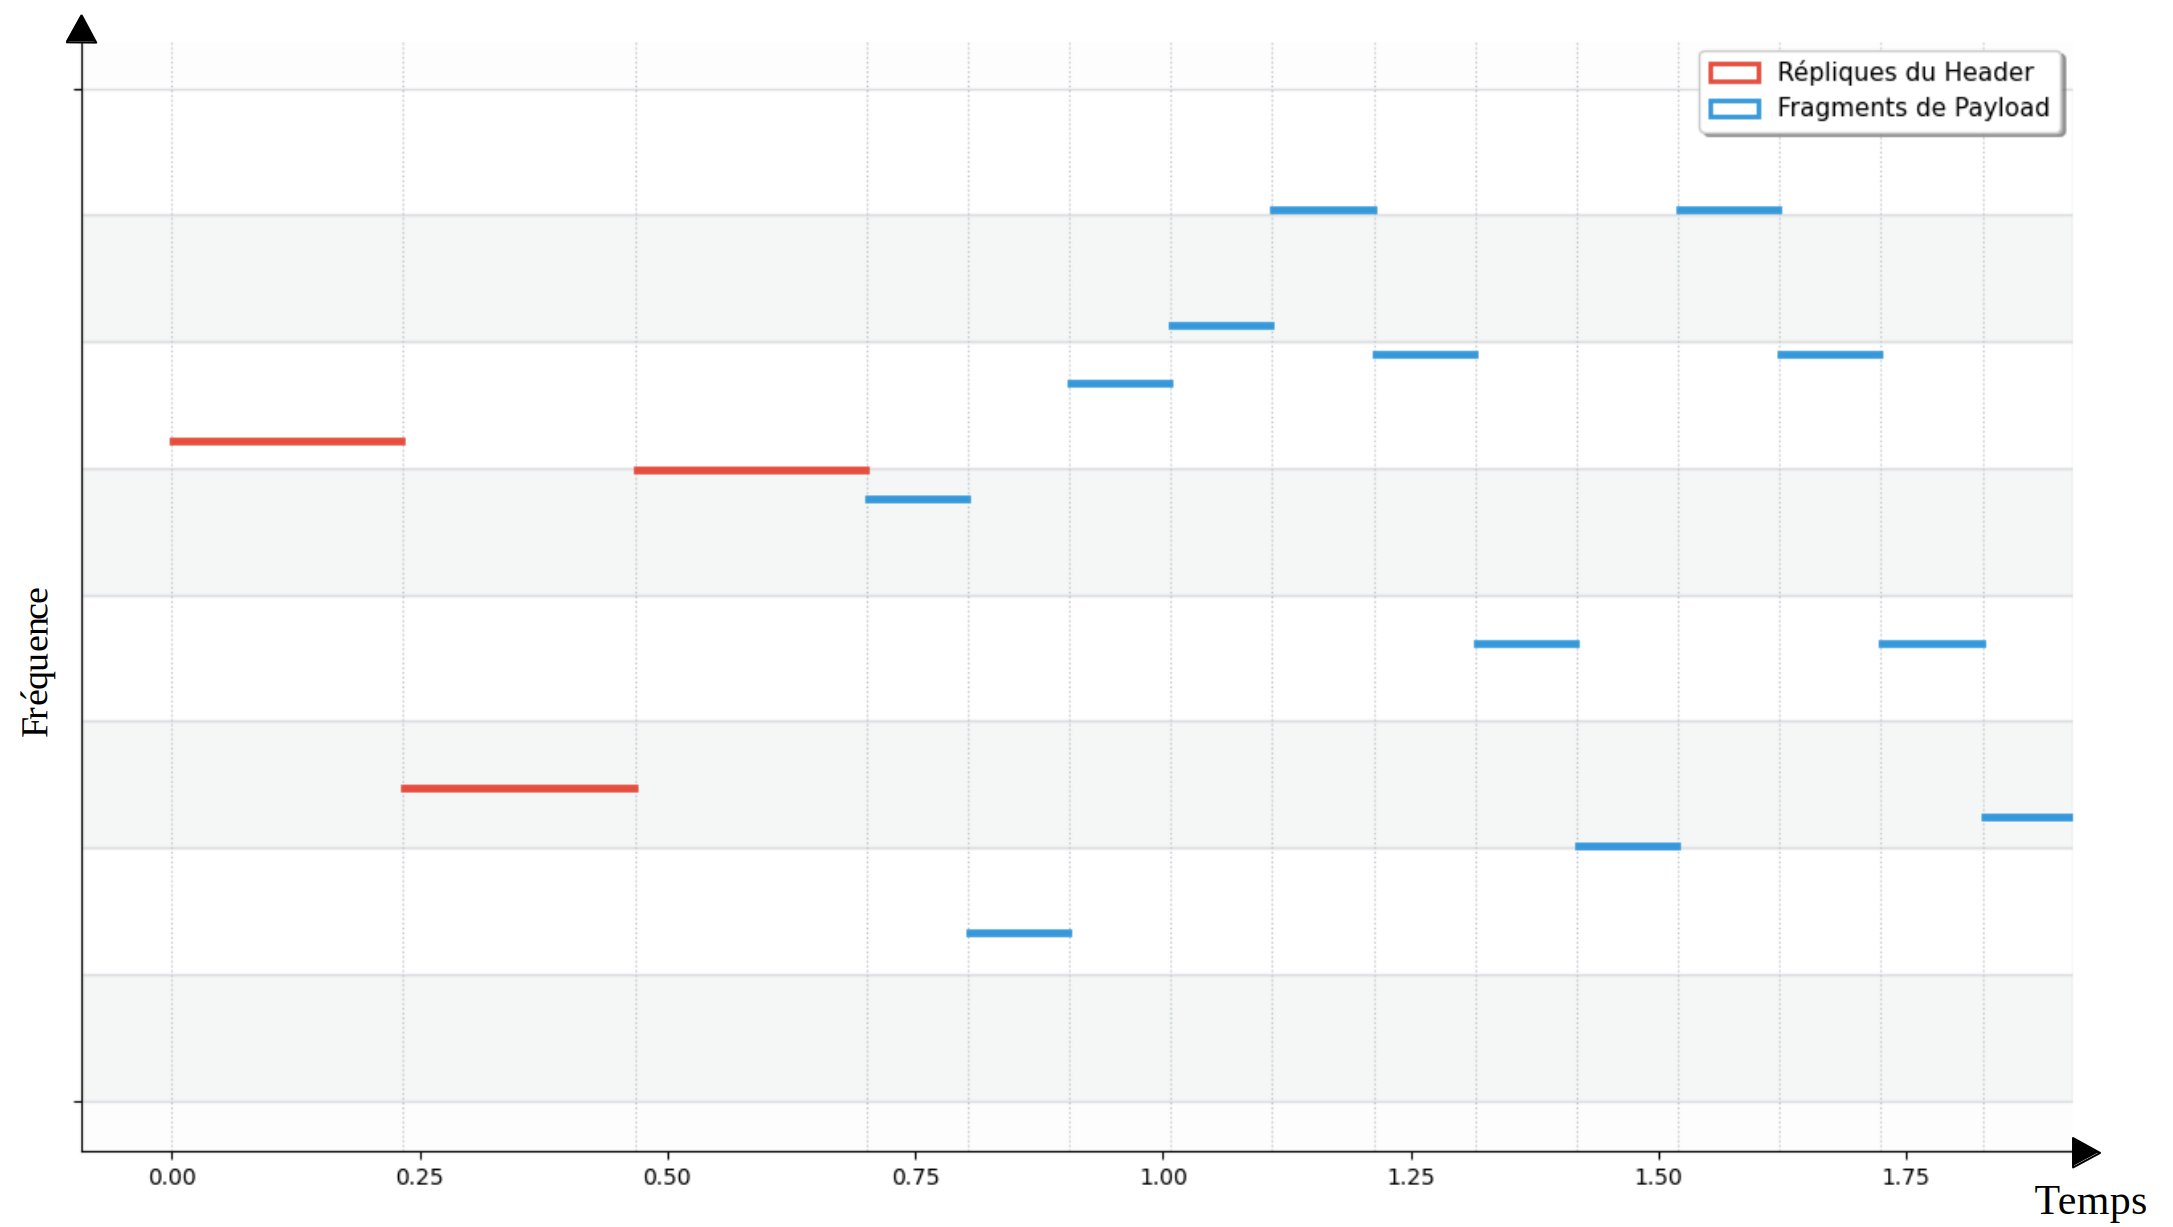
\includegraphics[width=1\textwidth]{images/lr_fhss_hop.png}
	\caption{Illustration des sauts de fréquence LR-FHSS}
	\label{fig:lr_fhss_hop}
\end{figure}

\section{Calcul du temps d'antenne}
Le temps d’antenne (Time on Air – ToA) constitue un paramètre essentiel dans l’analyse des performances des transmissions LR-FHSS. Cette section présente d’abord l’importance du temps d’antenne dans les réseaux IoT, puis introduit la formule générale permettant de le calculer avant de détailler le calcul du temps associé à la charge utile.

\subsection{Importance du temps d'antenne}

Dans les réseaux IoT, le temps d'antenne ($ToA$) est une métrique critique pour deux raisons principales :

\begin{itemize}
	\item \textbf{Respect de la réglementation} : Les bandes ISM (Industrial, Scientific and Medical) utilisées par LoRaWAN sont soumises à des contraintes de \textit{duty cycle}, limitant le pourcentage de temps pendant lequel un dispositif peut émettre (typiquement 1\% en Europe). Un $ToA$ élevé réduit donc la fréquence à laquelle un capteur peut transmettre.
	
	\item \textbf{Consommation énergétique} : La radio étant le composant le plus énergivore d'un capteur IoT, minimiser le $ToA$ est essentiel pour prolonger la durée de vie de la batterie.
\end{itemize}
\subsection{Formule générale}

Le temps d'antenne total d'un paquet LR-FHSS se décompose en deux parties : le temps de transmission de l'en-tête et le temps de transmission de la charge utile. La formule générale s'écrit :

\[ ToA = T_{header} + T_{payload} \]

où :

\[ T_{header} = N \times 233{,}472\,\text{ms} \]

avec $N$ le nombre de répétitions de l'en-tête ($N=3$ pour CR 1/3, $N=2$ pour CR 2/3).

\subsection{Calcul du temps de la charge utile}

Le calcul du temps de la charge utile, $T_{\text{payload}}$ est plus complexe, car il dépend de la longueur du message, du taux de codage et de la structure de fragmentation. Les formules suivantes sont extraites de la spécification RP002-1.0.5 \cite{loraalliance2025regional} :

\begin{itemize}
	\item \textbf{Pour CR = 1/3} :
	\begin{equation}
		\label{eq:toa1}
		 T_{payload} = \frac{(8 \times (L + 2) + 6) \times 3 + \left\lceil \frac{(8 \times (L + 2) + 6) \times 3}{48} \right\rceil \times 2}{50} \times 102{,}4\,\text{ms}
	\end{equation}
	
	
	\item \textbf{Pour CR = 2/3 (débit élevé)} :
	\begin{equation}
		\label{eq:toa2}
		 T_{payload} = \frac{\frac{(8 \times (L + 2) + 6) \times 3}{2} + \left\lceil \frac{(8 	\times (L + 2) + 6) \times 3}{2 \times 48} \right\rceil \times 2}{50} \times 102{,}4\,\text{ms} 
	\end{equation}
	
\end{itemize}

où $L$ est la longueur du message en octets (sans compter le CRC de 2 octets ajouté automatiquement).

Ces formules reflètent les opérations successives appliquées aux données :

\begin{enumerate}
	\item \textbf{$(8 \times (L + 2) + 6)$} : Calcul du nombre total de bits à transmettre, incluant le message ($L$ octets), le CRC (2 octets) et quelques bits supplémentaires de bourrage.
	
	\item \textbf{Multiplication par 3 ou par 3/2} : Application du codage convolutionnel qui ajoute de la redondance. Un taux 1/3 signifie que chaque bit d'information génère 3 bits codés.
	
	\item \textbf{Division par 48 et arrondi supérieur} : Découpage en blocs de 48 bits codés (un fragment), avec ajout d'un fragment supplémentaire si nécessaire.
	
	\item \textbf{Multiplication par 102,4 ms} : Durée d'un fragment.
\end{enumerate}

\section{Performances et capacité du LR-FHSS}
Cette section présente les performances et la capacité du LR-FHSS. Elle examine d’abord les apports théoriques issus de la littérature, puis détaille les validations expérimentales dans différents contextes, y compris les scénarios satellitaires, et enfin discute de l’efficacité énergétique du système.

\subsection{Apports théoriques}

L'architecture du LR-FHSS offre des avantages majeurs par rapport au LoRa. Plusieurs études académiques ont démontré ses bénéfices théoriques :

\subsubsection{Capacité réseau décuplée}

Dans cette étude \cite{lr_fhss_overview}, les auteurs ont réalisé une analyse comparative détaillée entre LoRa CSS et LR-FHSS. Leurs travaux montrent que, grâce à la granularité spectrale fine (488 Hz par fragment contre 125 kHz pour un canal LoRa classique), le LR-FHSS peut théoriquement supporter jusqu'à dix fois plus de dispositifs dans un même environnement. Cette multiplication de la capacité s'explique par deux phénomènes :

\begin{itemize}
	\item \textbf{Réduction des collisions} : La probabilité que deux dispositifs utilisent exactement les mêmes sous-canaux au même instant est considérablement réduite. Même en cas de collision partielle (quelques fragments communs), les fragments non corrompus peuvent parfois suffire à reconstruire le message grâce au codage convolutionnel.
	
	\item \textbf{Utilisation optimale du spectre} : Le saut aléatoire généré par l'algorithme \textit{Linear Feedback Shift Register (LFSR)} \cite{lfsr} garantit une distribution uniforme de la charge sur l'ensemble du spectre disponible.
\end{itemize}

Dans l'étude \cite{arxiv_lrfhss_2020}, les auteurs ont confirmé ces résultats par des modélisations analytiques, établissant des bornes théoriques sur le nombre maximal de dispositifs supportés en fonction du taux de charge offert et de la configuration choisie (DR, CR).

\subsubsection{Robustesse aux interférences}

La fragmentation et la dispersion fréquentielle confèrent au LR-FHSS une robustesse exceptionnelle face aux interférences, qu'elles soient d'origine naturelle (bruit impulsif, affaiblissement sélectif en fréquence) ou anthropique (brouilleurs, autres systèmes radio).

Semtech, dans sa note d'application AN1200.64 \cite{semtech2022lrfhss}, montre que le LR-FHSS maintient un taux de réception élevé même en présence d'interférences sur les bandes étroites qui bloqueraient complètement un canal LoRa. Cette résilience s'explique par le fait qu'une interférence localisée en fréquence ne détruit qu'une partie des fragments LR-FHSS, le reste restant exploitable.

\subsection{Validation expérimentale}

Cette section analyse les performances et la capacité de cette modulation à travers trois aspects principaux : les apports théoriques mis en évidence dans la littérature, les validations expérimentales réalisées dans différents scénarios, ainsi que l’efficacité énergétique du système.

\subsubsection{Analyses réelles}

La validation expérimentale est cruciale pour confirmer les performances réelles du LR-FHSS. À cet égard, les auteurs de l'étude \cite{lr_fhss_traces} ont mené une analyse approfondie sur des traces de paquets capturées en conditions réelles auprès de réseaux opérationnels. Leurs résultats confirment l'utilisation équitable du spectre, les mesures démontrant que tous les sous-canaux sont sollicités de manière équiprobable grâce au saut de fréquence aléatoire. 

Par ailleurs, l'étude révèle que les collisions partielles, limitées à quelques fragments, sont nettement plus fréquentes que les collisions totales ; grâce à la robustesse du codage, la majorité de ces interférences ne compromettent pas la récupération du message. Enfin, les auteurs soulignent une sensibilité marquée des performances vis-à-vis du choix des débits de données (DR) et du taux de codage (CR).

Une autre contribution majeure à la validation expérimentale a été apportée par cette étude \cite{lrfhss_comparaison}, où les auteurs ont réalisé une campagne de mesures comparative entre le LR-FHSS et le LoRa. L'étude montre que, dans des scénarios de non-ligne de vue (NLoS), le LR-FHSS (particulièrement aux DR8 et DR10) maintient une connectivité fiable jusqu'à 4 km, là où le LoRa (même au SF12) subit une perte totale de signal dès 2 km.

\subsubsection{Scénarios satellitaires}

L'un des cas d'usage les plus prometteurs du LR-FHSS concerne les communications directes avec des satellites en orbite basse terrestre. Ce scénario, extrêmement exigeant en raison de l'effet Doppler (décalage de fréquence), de l'atténuation de l'espace libre et des contraintes de puissance d'émission, constitue un cadre d'essai idéal pour évaluer la robustesse du LR-FHSS.

Dans l'étude \cite{lepcha_application_2021}, il est clairement démontré que l'utilisation de satellites en orbite basse pour la collecte de données dans des zones reculées et à faible coût avec LoRaWAN est faisable. Cela confirme naturellement les performances attendues du LR-FHSS, conçu d'une part pour répondre à ce besoin spécifique.

Les auteurs dans \cite{ieee_lr_fhss_2021} ont simulé des liaisons montantes LoRaWAN vers des satellites LEO en intégrant les effets physiques réels (Doppler, bruit thermique, fenêtre de visibilité). Leurs résultats démontrent que le LR-FHSS, en particulier avec CR 1/3, peut maintenir un lien fiable même dans ces conditions hostiles, là où le LoRa CSS peine à assurer la connectivité.

Dans cette étude \cite{lr_fhss_dts}, les auteurs ont approfondi cette analyse en comparant différentes configurations de LR-FHSS et en évaluant l'impact de paramètres orbitaux (altitude, inclinaison) sur les performances. Ils concluent que le LR-FHSS représente une solution viable pour l'IoT spatial, à condition d'optimiser la sélection des paramètres en fonction des contraintes.

Plus récemment, dans ce travail \cite{doppler_limits}, les auteurs ont étudié les limites fondamentales imposées par l'effet Doppler sur le LR-FHSS dans un contexte satellitaire. Ils montrent que, moyennant des techniques de pré-compensation ou de correction adaptative, le LR-FHSS peut fonctionner sur des liaisons satellitaires avec des vitesses relatives de plusieurs km/s, ouvrant ainsi la voie à des constellations massives de satellites à basse altitude pour l'IoT global.

\subsection{Efficacité énergétique}

À première vue, le LR-FHSS semble moins avantageux que le LoRa CSS en raison d’un temps d’antenne (ToA) plus long, augmentant ainsi la consommation d’énergie par paquet. Ce constat est d'autant plus vrai au-delà de +14 dBm, seuil à partir duquel l’amplificateur haute puissance (HPA) provoque une hausse marquée du courant \cite{ullah2024_energy}. Toutefois, cette analyse isolée du temps de transmission n'est pas représentative. Grâce à sa forte robustesse face aux interférences et à l’effet Doppler, le LR-FHSS limite considérablement les retransmissions. 

En tenant compte de la probabilité réelle de succès, le LR-FHSS en DR9 peut ainsi consommer moins d’énergie par paquet transmis que le LoRa DR5 sur des liaisons longue distance, selon \cite{SanchezVital2024EnergyLRFHSS, ullah2024_energy}. Dans des conditions optimales (DR9 ou DR11, mode non acquitté, charge utile maximale), il est même possible d’atteindre une autonomie théorique de 16 ans avec une simple pile bouton pour une transmission quotidienne \cite{SanchezVital2024EnergyLRFHSS}. L’efficacité énergétique du LR-FHSS ne peut donc pas être évaluée uniquement à partir du $ToA$, mais doit être appréciée de manière globale, en intégrant la fiabilité du lien, la taille des données transmises et la périodicité des envois.

\section{Conclusion}

Ce chapitre a présenté en détail les spécifications techniques du protocole LR-FHSS. Nous avons exploré les principes fondamentaux de cette technologie, depuis son architecture physique basée sur le saut de fréquence intra-paquet jusqu'à ses performances validées expérimentalement.

La compréhension approfondie des mécanismes du LR-FHSS, acquise dans ce chapitre, constitue le socle indispensable pour concevoir et évaluer des solutions d'optimisation. Les spécifications techniques présentées ici serviront de référence tout au long de ce mémoire, guidant nos choix de modélisation et de validation expérimentale.
	%% ============================================================================
%% CHAPITRE 3 : ÉTAT DE L'ART SUR L'OPTIMISATION DES PERFORMANCES DU LR-FHSS
%% ============================================================================
\chapter{ÉTAT DE L'ART SUR L'OPTIMISATION DES PERFORMANCES DU LR-FHSS}
\label{chap3}

\section{Introduction}
Le \gls{lrfhss} constitue une avancée majeure pour l'IoT satellitaire et les réseaux terrestres à très haute densité. Pourtant, plusieurs verrous limitent encore son plein potentiel : perte des en-têtes de trames, sensibilité à l'effet Doppler, rareté des ressources de démodulation à bord des passerelles, et absence de mécanismes d'adaptation dynamique aux conditions du canal.

Dans ce chapitre, nous analysons les travaux d'optimisation du LR-FHSS selon une approche critique. Pour chaque article, nous abordons le contexte, la problématique, la solution apportée et les résultats obtenus, avant d'en identifier les limites.

% ============================================================================
% ARTICLE 1 : RÉCEPTEUR AMÉLIORÉ ET DÉCODAGE SANS EN-TÊTE
% ============================================================================

\section{Récepteur LR-FHSS amélioré}

Les récepteurs LR-FHSS conventionnels nécessitent qu'au moins une réplique de l'en-tête soit bien reçue pour décoder un paquet. Dans les environnements denses, terrestres ou satellitaires, les collisions sur les en-têtes deviennent le principal facteur limitant les performances. La problématique centrale est donc de récupérer des trames LR-FHSS dont tous les en-têtes sont perdus, tout en prenant en compte les effets \textit{Doppler} caractéristiques des liaisons satellite.

\subsection{Architecture de récepteur augmenté}

Les auteurs de l'étude \cite{maldonado2025headerless} proposent la première architecture de récepteur capable de décoder des trames sans en-tête. Leur contribution repose sur trois éléments clés :

\begin{itemize}
	\item \textbf{Modélisation réaliste du canal spatial :} Intégration des effets Doppler spécifiques aux satellites en orbite basse terrestre (LEO), avec une modélisation précise du décalage en fréquence et de sa variation temporelle.
	
	\item \textbf{Algorithme glouton temps-fréquence :} Un algorithme de recherche exhaustive qui explore simultanément les dimensions temporelles, fréquentielles et les séquences de saut (FHS) pour localiser les fragments orphelins dans la matrice de réception $\mathcal{M}_N$.
	
	\item \textbf{Traitement différentiel :} Des modules de soustraction des trames déjà décodées ($\mathcal{M}_S$) de la matrice originale, isolant ainsi les fragments sans en-tête ($\mathcal{M}_C$), suivis d'un décodage exhaustif pour les deux taux de codage (CR1/3 et CR2/3).
\end{itemize}

\subsection{Résultats et analyse}

Les simulations montrent de bons résultats :

\begin{itemize}
	\item \textbf{Gain de 50\% du taux de paquets décodés} en contexte terrestre et spatial par rapport à un récepteur conventionnel.
	\item Le \textit{Doppler} agit comme un discriminant naturel : dans le scénario spatial, la dimension fréquentielle supplémentaire permet à l'algorithme de localisation d'atteindre un score F1 proche de 1 jusqu'à 800 transmissions simultanées.
	\item \textbf{Estimation fiable des trames sans en-tête jusqu'à 60\% d'occupation du canal}, au-delà de laquelle les faux positifs commencent à dégrader les performances.
\end{itemize}


Malgré son efficacité, cette approche peut présenter une limitation importante : la nécessité de modifier profondément l'architecture du récepteur (passerelle ou satellite), ce qui est complexe à déployer à grande échelle.

% ============================================================================
% ARTICLE 2 : SÉQUENCES DE SAUT ET ALLOCATION DE DÉMODULATEURS
% ============================================================================
\section{Optimisation des séquences de saut et d'allocation des démodulateurs}

La scalabilité du LR-FHSS repose fondamentalement sur deux éléments : les séquences de saut de fréquence (FHS), qui déterminent comment les fragments se répartissent sur le spectre, et les démodulateurs, ressources limitées à bord des passerelles. La problématique consiste à améliorer la capacité réseau en optimisant conjointement ces deux aspects.

\subsection{Rétro-ingénierie des séquences pilotes}

Les auteurs de l'étude \cite{maldonado2025enhancing} ont réalisé un travail de rétro-ingénierie des FHS utilisées dans les pilotes des modules LR-FHSS, révélant des informations cruciales :

\begin{itemize}
	\item Contrairement aux hypothèses de travaux antérieurs qui supposaient des séquences pseudo-aléatoires ou issues de fonctions de hachage \cite{lr_fhss_overview}, les FHS sont en réalité construites à partir de registres à décalage à rétroaction linéaire (LFSR) \cite{lfsr} produisant des \textit{m-séquences}.
	\item Les familles de séquences ainsi générées sont limitées à 384 dans les configurations standards, ce qui constitue un goulot d'étranglement potentiel.
	\item Les auteurs ont publié un outil open-source permettant de générer ces séquences, facilitant ainsi leur analyse et leur amélioration par la communauté.
\end{itemize}

\subsection{Nouvelles familles de séquences optimisées}

Avec cette compréhension approfondie, les auteurs proposent de nouvelles familles de FHS optimisées pour le LR-FHSS :

\begin{itemize}
	\item \textbf{Familles Lempel-Greenberger :} Basées sur les constructions optimales de corrélation de \textit{Hamming}, générant 32 à 64 séquences de longueur 31.
	\item \textbf{Familles Li-Fan (Wide-Gap sequences) :} Conçues pour garantir un écart minimal entre les sauts de fréquence successifs, en conformité avec les régulations (écart de 3,9 kHz en Europe). Ces familles, construites selon les méthodes $2\ell$ et $3\ell$, produisent entre 18 et 107 séquences adaptées aux contraintes du LR-FHSS.
\end{itemize}

\subsection{Stratégies d'allocation dynamique des démodulateurs}

En complément de l'optimisation des séquences, les auteurs introduisent deux stratégies novatrices pour l'allocation des ressources de démodulation :

\begin{itemize}
	\item \textbf{Early-Decode :} Le démodulateur commence le décodage dès qu'il a collecté le nombre minimum de fragments requis (33\% pour CR1/3, 67\% pour CR2/3), au lieu d'attendre la fin de la réception de tous les fragments. Cette libération anticipée de la ressource permet de traiter plus de trames simultanément.
	
	\item \textbf{Early-Drop :} Si le démodulateur détecte qu'il est impossible d'atteindre le seuil de fragments nécessaires (trop de collisions déjà observées), il abandonne prématurément la réception du paquet, libérant ainsi la ressource pour d'autres trames plus prometteuses.
\end{itemize}

\subsection{Résultats et analyse}

Les simulations exhaustives menées par les auteurs, avec des configurations allant de 100 à 1000 démodulateurs et différents taux de codage, produisent des résultats remarquables :

\begin{itemize}
	\item \textbf{Gain de capacité de décodage jusqu'à 100\%} avec 100 démodulateurs et l'activation conjointe des mécanismes Early-Decode/Early-Drop.
	\item La famille \textbf{Li-Fan surpasse la famille pilote d'origine de 170\%} en configuration dense (CR2/3) avec 1000 démodulateurs.
	\item La \textbf{tolérance aux collisions sur en-tête} (simulation d'une robustesse accrue de 4 time-slots) double les performances dans les scénarios à forte densité.
	\item Analyse comparative détaillée montrant que la famille Li-Fan est particulièrement avantageuse pour les charges réseau élevées, tandis que la famille pilote conserve un léger avantage pour les faibles densités.
\end{itemize}

\subsection{Limites de l'approche}

Ces avancées significatives présentent néanmoins des limites importantes :

\begin{itemize}
	\item L'optimisation reste fondamentalement \textbf{statique} : la conception des séquences est effectuée une fois pour toutes (\textit{offline}), indépendamment des conditions de propagation et de la densité du réseau.
	\item Les stratégies d'allocation, bien que dynamiques dans leur exécution, suivent des règles prédéfinies qui ne s'adaptent pas aux variations du canal (ombrage, évanouissements).
	\item La mise en œuvre effective de leur stratégie nécessitera une modification profonde des dispositifs. 
\end{itemize}

% ============================================================================
% ARTICLE 3 : PRÉ-COMPENSATION DOPPLER CÔTÉ TERMINAL
% ============================================================================
\section{Pré-compensation Doppler pour liaisons directes vers satellite}

L'effet Doppler constitue la principale cause de perte de synchronisation et de paquets dans les liaisons satellitaires. La question centrale est de savoir s’il est possible de compenser ce décalage de manière logicielle, sans recourir à un module GNSS (Global Navigation Satellite System) à la fois coûteux et énergivore. L'enjeu est d'y parvenir sans modification matérielle tout en garantissant un surcoût énergétique négligeable.

\subsection{Méthode de pré-compensation par balises Doppler}

Les auteurs de l'étude \cite{ullah_extending_doppler_2025} proposent une solution pratique : la pré-compensation via des balises Doppler (\textit{Doppler Beacons}). Leur approche se décompose en plusieurs étapes :

\begin{enumerate}
	\item \textbf{Émission continue de balises :} Le satellite émet en permanence des balises constituées d'un simple préambule LoRa (8,25 symboles minimum), sans charge utile ni CRC, sur une large bande ($B_{downlink} = 500$ kHz) garantissant une réception robuste malgré le Doppler.
	
	\item \textbf{Mesure du décalage :} L'équipement terrestre ouvre une fenêtre de réception (RX0) avant chaque transmission montante et utilise la fonction \gls{fei} (Frequency Error Indicator) intégrée aux puces LoRa pour mesurer précisément le décalage Doppler subi par la balise.
	
	\item \textbf{Pré-compensation :} L'équipement ajuste sa fréquence d'émission $f'(t)$ selon la formule :
	\[f'(t) = f_c' + f_d(t)\left(\frac{f_c'}{f_c}\right)\]
	où $f_c$ et $f_c'$ sont les fréquences porteuses descendante et montante, et $f_d(t)$ le décalage mesuré.
\end{enumerate}

\subsection{Validation sur données réelles}

La force de cette étude réside dans sa validation à partir de données de télémétrie réelles des satellites TIANQI-7 et TIANQI-27, via la plateforme ouverte TinyGS :

\begin{itemize}
	\item \textbf{Données exploitées :} Plus de 2 millions de paquets confirmés, avec des périodes d'émission de 15 secondes, couvrant des altitudes de 518 km (TIANQI-7) et 904 km (TIANQI-27).
	\item \textbf{Traitement :} Interpolation et extrapolation des mesures FEI discrètes pour couvrir l'intégralité de la fenêtre de visibilité satellite.
\end{itemize}

\subsection{Résultats obtenus}

Les résultats démontrent l'efficacité remarquable de la méthode :

\begin{itemize}
	\item \textbf{Élimination complète des pertes dues au décalage Doppler} pour des liens montants avec des largeurs de bande étroites (31,25 kHz), sur des altitudes de 200 à 518 km et des fréquences de 401 MHz à 2 GHz.
	\item \textbf{Surcoût énergétique marginal} de seulement 2,5\% pour l'équipement terrestre, préservant une durée de vie de batterie supérieure à 5 ans.
	\item Analyse détaillée des paramètres optimaux : la bande passante minimale requise pour les balises varie de 43,6 kHz à 433 MHz jusqu'à 201,5 kHz en bande S (2 GHz).
\end{itemize}

\subsection{Limites de l'approche}

Cette solution, bien qu'extrêmement efficace pour le problème spécifique du Doppler, présente des limites dans le cadre plus large de notre problématique :

\begin{itemize}
	\item Elle n'offre aucun mécanisme d'optimisation de la puissance d'émission ou du débit de données en fonction des conditions de propagation.
	\item L'adaptation se limite à la compensation fréquentielle, sans considération pour la fiabilité globale ou l'efficacité énergétique.
\end{itemize}

% ============================================================================
% ARTICLE 4 : APPROCHES PAR APPRENTISSAGE ET SAUT DE FRÉQUENCE GÉNÉRIQUE
% ============================================================================
\section{Optimisation par apprentissage et saut de fréquence}

Les travaux récents abordent une problématique double dans l'optimisation des réseaux LoRaWAN. Celle-ci consiste, d'une part, à intégrer le saut de fréquence au sein des communications LoRa, et d'autre part, à mettre en œuvre un agent basé sur l'apprentissage par renforcement profond capable de sélectionner de manière optimale les paramètres de transmission. L'objectif commun à ces deux mécanismes est l'amélioration de l'efficacité énergétique du réseau.

\subsection{Algorithmes proposés}

Les études \cite{greenlora,greenlora2024} proposent deux algorithmes complémentaires :

\begin{itemize}
	\item \textbf{LoRa-DDPG-FHSS} \cite{greenlora} : Un algorithme d'ordonnancement basé sur le \textit{Deep Deterministic Policy Gradient}(DDPG) qui optimise un quadruplet (Canal, SF, TP, Time Slot) pour chaque transmission. L'agent apprend une politique minimisant l'énergie consommée tout en évitant les collisions.
	
	\item \textbf{DP-FH (Deterministic Policy - Frequency Hopping)} \cite{greenlora2024} : Une version améliorée qui affine la sélection des paramètres en intégrant des informations d'état plus complètes (localisation des nœuds, taille des buffers de données) et en utilisant une architecture de réseau de neurones optimisée.
\end{itemize}

\subsection{Résultats}

Les simulations, réalisées avec l'outil LoRaSim, montrent des gains spectaculaires :

\begin{itemize}
	\item \textbf{Efficacité énergétique multipliée par 98} par rapport à l'algorithme heuristique FREE \cite{free}.
	\item \textbf{Réduction du temps d'antenne de 97\%}, libérant ainsi les ressources spectrales.
	\item \textbf{Amélioration du PDR de 42\%}, démontrant que l'optimisation énergétique ne se fait pas au détriment de la fiabilité.
	\item \textbf{Diminution des collisions de 9\%}, grâce à une allocation plus intelligente des ressources.
	\item Analyse détaillée de la distribution des facteurs d'étalement (SF) montrant que l'agent privilégie les SF faibles (SF7 pour 75\% des nœuds) pour minimiser l'énergie, n'utilisant les SF élevés que pour les nœuds éloignés.
\end{itemize}

\subsection{Limites et incompatibilités majeures avec le LR-FHSS}

Malgré ces résultats impressionnants, ces travaux présentent des limitations fondamentales qui les rendent inapplicables directement au LR-FHSS :

\begin{enumerate}
	\item Ces travaux présentent une ambiguïté conceptuelle dans la distinction entre LoRa CSS et LR-FHSS.
	\item \textbf{Incompatibilité des paramètres optimisés :} L'agent optimise le \textit{Spreading Factor (SF)}, paramètre central du LoRa CSS mais inexistant en LR-FHSS. Cette technologie utilise la modulation GMSK avec des débits de données fixes (DR8, DR9, DR10, DR11, etc.) dont les propriétés de robustesse sont fondamentalement différentes.
	
	\item \textbf{Modèle physique inadapté :} Le simulateur LoRaSim et son modèle de collision sont conçus pour la modulation CSS. Ils ne capturent pas les spécificités du LR-FHSS : structure en-têtes/fragments, probabilité de succès par fragment, effet du codage convolutionnel, et mécanisme de saut intra-paquet.
	
	\item \textbf{Métriques non représentatives :} Les gains annoncés, bien que spectaculaires, ne peuvent être directement transposés au contexte LR-FHSS en raison des différences fondamentales de couche physique.
\end{enumerate}

\subsection{Apport pour notre travail}

Malgré ces limitations, ces travaux apportent des contributions précieuses pour notre travail :

\begin{itemize}
	\item Ils démontrent que le saut de fréquence est un levier d'optimisation puissant pour les réseaux longue portée.
	\item Ils confirment la pertinence de l'apprentissage par renforcement profond pour l'allocation dynamique de ressources dans des environnements complexes.
	\item Ils fournissent un cadre méthodologique (formulation MDP, conception de la récompense, architecture acteur-critique) dont nous pouvons nous inspirer.
\end{itemize}

% ============================================================================
% SYNTHÈSE ET POSITIONNEMENT
% ============================================================================
\section{Synthèse critique et positionnement de nos travaux}
Il apparaît clairement qu'aucune solution existante ne propose une optimisation dynamique, multi-objectifs (fiabilité et énergie) et spécifiquement adaptée aux mécanismes physiques du LR-FHSS. Les approches par apprentissage, bien que prometteuses, souffrent d'une incompatibilité fondamentale avec les paramètres réels du LR-FHSS.

Le tableau \ref{tab:synthèse_etat_art} synthétise les approches existantes et met en évidence leurs limites respectives.

\begin{table}[H]
	\centering
	\caption{Synthèse critique des approches d'optimisation du LR-FHSS}
	\label{tab:synthèse_etat_art}
	\begin{tabular}{|p{3cm}|p{4cm}|p{3cm}|p{4cm}|}
		\hline
		\textbf{Approche / Référence} & \textbf{Principe} & \textbf{Avantages} & \textbf{Limites} \\
		\hline
		Récepteur augmenté \cite{maldonado2025headerless} & Décodage de trames sans en-tête & +50\% de PDR & Modification du récepteur \\
		\hline
		FHS optimisées \cite{maldonado2025enhancing} & Nouvelles séquences et allocation démodulateurs & +100\% de capacité, Li-Fan +170\% & Optimisation \textit{statique} (offline) \\
		\hline
		Pré-compensation Doppler \cite{ullah_extending_doppler_2025} & Balises Doppler pour ajustement fréquence & Élimination des pertes Doppler, surcoût énergétique 2,5\% & Solution spécifique au seul problème Doppler \\
		\hline
		RL pour LoRa-FHSS \cite{greenlora,greenlora2024} & Agent DDPG pour (Canal, SF, TP, Slot) & Gains énergétiques ×98, -97\% ToA & \textbf{Incompatible avec LR-FHSS} (SF, modèle CSS) \\
		\hline
	\end{tabular}
\end{table}

Notre travail se positionne pour combler cette lacune. Il reprend l'idée de l'optimisation par apprentissage profond, validée par \cite{greenlora,greenlora2024}, mais la rend applicable et pertinente pour le LR-FHSS.

\section{Conclusion}
Dans ce chapitre, nous avons présenté une revue critique de l'état de l'art sur l'optimisation du LR-FHSS. En montrant les avancées dans ce domaine, nous avons également mis en lumière les limites et imprécisions des différentes propositions et ainsi évoqué le positionnement de notre travail face à ce constat.
	\chapter{PRÉSENTATION ET IMPLÉMENTATION DE LA SOLUTION}

\section{Introduction}
\label{sec:intro-ddqn}

Ce chapitre présente la conception et l'implémentation d'un agent d'apprentissage par renforcement basé sur l'algorithme \gls{ddqn} (\textit{Double Deep Q-Network}) pour l'optimisation des transmissions LR-FHSS. Nous détaillons la formulation du problème en tant que processus de décision markovien, l'architecture du réseau de neurones, l'environnement d'entraînement et l'algorithme d'apprentissage.

\section{Problématique et formalisme MDP}
\label{sec:problematique-mdp}
Notre travail vise à assurer la fiabilité et l'efficacité énergétique des transmissions dans les réseaux LoRaWAN utilisant LR-FHSS. Nous proposons pour cela une approche basée sur l'apprentissage par renforcement profond (DRL), où un agent intelligent, situé sur un serveur de bordure, apprend une politique de transmission optimale à travers son interaction avec l'environnement.

\subsection{Formulation en processus de décision markovien}
\label{subsec:formulation-mdp}

Le problème d'optimisation des transmissions LR-FHSS peut être formulé comme un \gls{mdp} (\textit{Markov Decision Process}). Un MDP est un cadre mathématique pour modéliser la prise de décision séquentielle dans un environnement où les résultats sont en partie aléatoires et en partie sous le contrôle de l'agent. Il est formellement défini par le tuple $(\mathcal{S}, \mathcal{A}, \mathcal{P}, \mathcal{R}, \gamma)$ \cite{puterman1994mdp,sutton2018reinforcement} :

\begin{itemize}
	\item \textbf{$\mathcal{S}$ : L'espace d'états}. Il représente l'ensemble des informations pertinentes dont dispose l'agent au moment de prendre une décision. Dans notre cas, l'état capture la situation d'un nœud avant une transmission.
	
	\item \textbf{$\mathcal{A}$ : L'espace d'actions}. Il s'agit de l'ensemble des choix discrets disponibles pour l'agent. Ici, une action correspond à la sélection simultanée d'un débit de données et d'une puissance d'émission.
	
	\item \textbf{$\mathcal{P}(s' \mid s, a)$ : La dynamique de transition}. C'est la probabilité de passer de l'état $s$ à l'état $s'$ après avoir exécuté l'action $a$. Cette dynamique est régie par l'environnement (le simulateur) et est inconnue de l'agent.
	
	\item \textbf{$\mathcal{R}(s, a, s')$ : La fonction de récompense}. C'est un signal scalaire immédiat qui évalue la qualité de la transition de l'état $s$ à l'état $s'$ suite à l'action $a$. L'objectif de l'agent est de maximiser la somme de ces récompenses sur le long terme.
	
	\item \textbf{$\gamma \in [0, 1]$ : Le facteur d'actualisation (\textit{discount factor})}. Il détermine l'importance accordée aux récompenses futures par rapport aux récompenses immédiates. Un $\gamma$ proche de 1 rend l'agent ``prévoyant'', tandis qu'un $\gamma$ proche de 0 le rend ``court-termiste''.
\end{itemize}

L'objectif de l'agent est de trouver une politique $\pi^* : \mathcal{S} \rightarrow \mathcal{A}$ qui maximise l'espérance de la somme actualisée des récompenses futures :

\begin{equation}
	\pi^* = \arg\max_{\pi} \mathbb{E}_{\tau \sim \pi} \left[ \sum_{t=0}^{\infty} \gamma^t r_t \right]
\end{equation}

où $\tau = (s_0, a_0, r_0, s_1, a_1, r_1, \ldots)$ est une trajectoire (ou épisode) générée en suivant la politique $\pi$.

\subsection{\texorpdfstring{Définition de l'espace d'états $\mathcal{S}$}{Définition de l'espace d'états}}
\label{subsec:espace-etats}

L'état $s_t \in \mathbb{R}^8$ est un vecteur de huit variables normalisées, conçu pour fournir à l'agent une représentation concise mais complète de la situation d'un nœud avant une transmission. Chaque composante est choisie pour son influence sur la décision optimale.

\begin{figure}[H]
	\centering
	\begin{tikzpicture}[node distance=1.1cm, auto, >=latex]
		% --- Colonne de GAUCHE ---
		\node[rectangle, draw, fill=blue!10, minimum width=2.8cm, minimum height=0.7cm] (d_norm) {$d_{\text{norm}}$};
		\node[rectangle, draw, fill=blue!10, minimum width=2.8cm, minimum height=0.7cm, below of=d_norm] (snr_avg) {$\text{SNR}_{\text{avg}}$};
		\node[rectangle, draw, fill=blue!10, minimum width=2.8cm, minimum height=0.7cm, below of=snr_avg] (tau_success) {$\tau_{\text{success}}$};
		\node[rectangle, draw, fill=blue!10, minimum width=2.8cm, minimum height=0.7cm, below of=tau_success] (r_norm) {$r_{\text{norm}}$};
		
		% --- Colonne de DROITE ---
		\node[rectangle, draw, fill=blue!10, minimum width=2.8cm, minimum height=0.7cm, right=4cm of d_norm] (log_d) {$\log(d)_{\text{norm}}$};
		\node[rectangle, draw, fill=blue!10, minimum width=2.8cm, minimum height=0.7cm, below of=log_d] (t_day) {$t_{\text{day}}$};
		\node[rectangle, draw, fill=blue!10, minimum width=2.8cm, minimum height=0.7cm, below of=t_day] (sigma_snr) {$\sigma_{\text{SNR}}$};
		\node[rectangle, draw, fill=blue!10, minimum width=2.8cm, minimum height=0.7cm, below of=sigma_snr] (l_norm) {$L_{\text{norm}}$};
		
		% --- Point de jonction au milieu ---
		% On définit un point invisible au centre des deux colonnes
		\coordinate (center) at ($(r_norm.south)!0.5!(l_norm.south) + (0,-1)$);
		
		% --- Bloc ÉTAT (en bas au centre) ---
		\node[rectangle, draw, fill=green!10, minimum width=6cm, minimum height=1cm, below=1.5cm of center] (state) {État $s_t \in \mathbb{R}^8$};
		
		% --- Lignes GAUCHE (partent du côté gauche, contournent et rejoignent le centre) ---
		\foreach \i in {d_norm, snr_avg, tau_success, r_norm} {
			\draw[thick] (\i.west) -- ++(-0.5,0) |- (center);
		}
		
		% --- Lignes DROITE (partent du côté droit, contournent et rejoignent le centre) ---
		\foreach \i in {log_d, t_day, sigma_snr, l_norm} {
			\draw[thick] (\i.east) -- ++(0.5,0) |- (center);
		}
		
		% --- Flèche finale vers le vecteur d'état ---
		\draw[->, thick] (center) -- (state.north);
		
	\end{tikzpicture}
	\caption{Composition de l'espace d'états $\mathcal{S}$.}
	\label{fig:etat-vecteur}
\end{figure}

Le tableau~\ref{tab:state-space-ddqn} détaille chaque composante, sa plage de valeurs et sa justification.

\begin{table}[!ht]
	\centering
	\caption{Description détaillée des composantes de l'espace d'états.}
	\label{tab:state-space-ddqn}
	\begin{tabular}{|p{2.5cm}|p{2cm}|p{8cm}|}
		\hline
		\textbf{Variable} & \textbf{Plage} & \textbf{Description et justification} \\
		\hline
		$d_{\text{norm}}$ & [0, 1] & Distance à la passerelle normalisée par la portée maximale. La distance est le principal facteur influençant l'atténuation du signal. \\
		\hline
		$\text{SNR}_{\text{avg}}$ & [-1, 1] & Moyenne du SNR (\textit{Signal-to-Noise Ratio}) des trois dernières transmissions. Normalisée par une valeur typique de 20 dB. Indicateur direct de la qualité récente du lien. \\
		\hline
		$\tau_{\text{success}}$ & [0, 1] & Taux de succès des cinq dernières transmissions. Permet à l'agent d'ajuster sa stratégie en fonction de la performance récente. \\
		\hline
		$r_{\text{norm}}$ & [0, 1] & Nombre de retransmissions consécutives après un échec, normalisé par 5. Un nombre élevé indique des conditions de canal dégradées et doit inciter à une configuration plus robuste. \\
		\hline
		$\log(d)_{\text{norm}}$ & [0, 1] & Logarithme de la distance normalisé. L'atténuation du signal étant proportionnelle à $\log(d)$, cette transformation linéarise la relation et facilite l'apprentissage. \\
		\hline
		$t_{\text{day}}$ & [0, 1] & Variable de phase temporelle, prévue pour modéliser des variations diurnes du canal (activité humaine, interférences variables). Dans le cadre de cette étude, les simulations couvrent des durées inférieures à 24h et aucune variation temporelle du canal n'est implémentée ; cette composante reste donc constante et constitue une extension pour les travaux futurs.  \\
		\hline
		$\sigma_{\text{SNR}}$ & [0, 1] & Stabilité du signal, définie comme l'inverse de l'écart-type des trois derniers SNR. Un canal stable (valeur proche de 1) permet d'utiliser des configurations plus agressives. \\
		\hline
		$L_{\text{norm}}$ & [0, 1] & Taille de la charge utile (payload) en octets, normalisée par la taille maximale autorisée (123 octets). Influence directement le temps d'antenne (ToA) et donc le risque de collision. \\
		\hline
	\end{tabular}
\end{table}

La normalisation de toutes les composantes dans des plages bornées ($[0, 1]$ ou $[-1, 1]$) est essentielle pour stabiliser l'apprentissage du réseau de neurones. Elle évite que des variables avec de grandes amplitudes numériques ne dominent le processus de mise à jour des poids.

\subsection{\texorpdfstring{Définition de l'espace d'actions $\mathcal{A}$}{Définition de l'espace d'actions}}
\label{subsec:espace-actions}

L'espace d'actions $\mathcal{A}$ est un espace discret. Une action $a \in \mathcal{A}$ correspond à la sélection simultanée d'un DR et d'une puissance d'émission :

\begin{equation}
	\mathcal{A} = \underbrace{\{\text{DR}8, \text{DR}9, \text{DR}10, \text{DR}11\}}_{4 \text{ DR}} \times \underbrace{\{-4, -3, \dots, 13, 14\}}_{19 \text{ puissances}}
\end{equation}

Le nombre total d'actions est donc $|\mathcal{A}| = 4 \times 19 = 76$. Chaque action est encodée par un entier unique $a \in \{0, 1, \dots, 75\}$. Cet espace d'action discret est parfaitement adapté à l'algorithme \gls{dqn} et à ses dérivés. Il capture l'ensemble des configurations de transmission valides pour la bande EU868.

\subsection{Conception de la fonction de récompense}
\label{subsec:fonction-recompense}

La fonction de récompense est l'élément le plus critique de la formulation du \gls{mdp}. Elle traduit les objectifs de notre approche (fiabilité, efficacité énergétique et efficacité spectrale) en un signal d'apprentissage concret. Nous proposons une structure paramétrée permettant d'équilibrer ces objectifs souvent contradictoires par l'ajustement de coefficients de pondération.

La récompense totale $\mathcal{R}$ est définie de manière conditionnelle selon l'issue de la transmission :

\begin{equation}
	\mathcal{R} = 
	\begin{cases} 
		\phi & \text{si échec} \\
		\rho + \mathcal{R}_{\text{ToA}} + \mathcal{R}_{\text{power}} + \mathcal{R}_{\text{retry}} + \Omega(\text{SNR}, \text{DR}) & \text{si succès}
	\end{cases}
\end{equation}

Les composantes de cette fonction sont définies comme suit :

\begin{itemize}
	\item \textbf{Base de performance ($\phi, \rho$)} : 
	Le paramètre $\phi$ pénalise l'échec pour garantir la fiabilité, tandis que $\rho$ est la récompense de base pour un succès.
	\[ \phi = -200, \quad \rho = +100 \]
	Ces valeurs soulignent que l'échec est deux fois plus coûteux que le succès n'est gratifiant, forçant l'agent à privilégier la délivrance du paquet.
	
	\item \textbf{Pénalité d'occupation spectrale ($\mathcal{R}_{\text{ToA}}$)} :
	Elle pénalise le temps d'occupation du canal (temps d'antenne) normalisé par le ToA maximum théorique ($T_{max} = 3813.376$ ms).
	\begin{equation}
		\mathcal{R}_{\text{ToA}} = -\alpha \cdot \min\left(\frac{\text{ToA}_{\text{ms}}}{T_{max}}, 1\right) \quad \text{avec } \alpha = 80
	\end{equation}
	Cette pénalité encourage l'agent à minimiser la durée de ses transmissions, réduisant ainsi les risques de collision et améliorant l'efficacité énergétique et spectrale globale du réseau.
	
	\item \textbf{Pénalité d'efficacité énergétique ($\mathcal{R}_{\text{power}}$)} : 
	Elle sanctionne l'utilisation de puissances d'émission élevées sur la plage normalisée du matériel (ici de -4 à 14 dBm).
	\begin{equation}
		\mathcal{R}_{\text{power}} = -\beta \cdot \left( \frac{P_{\text{TX}} + 4}{18} \right) \quad \text{avec } \beta = 50
	\end{equation}
	
	\item \textbf{Pénalité de retransmission ($\mathcal{R}_{\text{retry}}$)} : 
	Elle incite l'agent à minimiser le nombre de tentatives ($N_{retry}$) pour réduire la congestion.
	\begin{equation}
		\mathcal{R}_{\text{retry}} = -\gamma \cdot (\frac{N_{retry}}{5}) \quad \text{avec } \gamma = 30
	\end{equation}
	
	\item \textbf{Optimisation de la qualité du lien ($\Omega$)} : 
	Ce terme regroupe les bonus de robustesse ($\mathcal{R}_{\text{SNR}}$) et d'efficacité spectrale ($\mathcal{R}_{\text{DR}}$) :
	
	\[ \mathcal{R}_{\text{SNR}} = 
	\begin{cases} 
		+\delta & \text{si } -5 \leq \text{SNR} \leq 5 \text{ dB (Optimal)} \\
		-\epsilon \cdot \max(0, \text{SNR} - 10) & \text{si } \text{SNR} > 10 \text{ dB (Overkill)} \\
		0 & \text{sinon}
	\end{cases} \]
	
	Avec $\delta = 20$ et $\epsilon = 4$. La zone de SNR ``optimale'' est définie comme une marge suffisante pour garantir la réception sans excès.
	
	\item \textbf{Bonus d'efficacité spectrale ($\mathcal{R}_{\text{DR}}$)} : Il favorise l'utilisation de \gls{dr} plus efficaces (ceux avec un \gls{cr} de 2/3) lorsque les conditions de canal le permettent.
	\begin{equation}
		\mathcal{R}_{\text{DR}} =
		\begin{cases}
			0 & \text{si DR} = 8 \\
			+10 & \text{si DR} = 9 \\
			+5 & \text{si DR} = 10 \\
			+15 & \text{si DR} = 11
		\end{cases}
	\end{equation}
\end{itemize}


L'utilisation de ces paramètres ($\alpha, \beta, \gamma, \delta, \epsilon$) permet de séparer la logique de décision de l'agent (stratégie LR-FHSS) des valeurs numériques concrètes. Cette séparation facilite l'ajustement et l'optimisation ultérieure de la politique de l'agent via des méthodes de recherche d'hyperparamètres, sans modifier la structure de la fonction de récompense elle-même.


\subsubsection{Analyse des poids relatifs des objectifs de la fonction de récompense}
\label{subsec:poids-relatifs-objectifs}

L'analyse des poids relatifs permet de quantifier l'importance de chaque objectif dans le processus d'apprentissage de l'agent. Les calculs sont basés sur les plages de variation de chaque composante.



\begin{table}[H]
	\centering
	\caption{Poids relatifs individuels des composantes de la récompense}
	\label{tab:poids-individuels}
	\begin{tabular}{|l|c|c|c|c|}
		\hline
		\textbf{Composante} & \textbf{Symbole} & \textbf{Plage} & \textbf{Poids absolu} & \textbf{Poids relatif} \\
		\hline
		Échec / Succès & $\phi, \rho$ & $[-200, +100]$ & 300 & 53,27\% \\
		\hline
		Retransmissions & $\gamma$ & $[-30, 0]$ & 30 & 5,33\% \\
		\hline
		Qualité du lien (SNR) & $\delta, \epsilon$ & $[-80, +20]$ & 100 & 17,76\% \\
		\hline
		Temps d'occupation (ToA) & $\alpha$ & $[-80, -11,82]$ & 68,18 & 12,10\% \\
		\hline
		Puissance d'émission & $\beta$ & $[-50, 0]$ & 50 & 8,88\% \\
		\hline
		Efficacité spectrale (DR) & — & $[0, +15]$ & 15 & 2,66\% \\
		\hline
		\textbf{TOTAL} & & & \textbf{563,18} & \textbf{100\%} \\
		\hline
	\end{tabular}
\end{table}

L’analyse des poids attribués aux différentes composantes de la fonction de récompense permet d’identifier clairement les priorités de l’agent :

\begin{enumerate}
	\item \textbf{Garantir la fiabilité des transmissions} :
	Le critère succès/échec représente à lui seul un poids de 53,27\%. En intégrant également la pénalité liée aux retransmissions, cette proportion atteint 58,6\%. Cela indique que l’objectif principal de l’agent consiste à maximiser le taux de transmissions réussies tout en limitant les retransmissions.
	
	\item \textbf{Optimiser l’efficacité spectrale et énergétique} :
	Le cumul des métriques associées à ces performances représente 41,4\% du poids total, constituant ainsi le second objectif majeur après la fiabilité. Par ailleurs, en tenant compte de l’impact indirect des retransmissions sur la consommation énergétique à long terme, cette valeur atteint 46,76\%.
\end{enumerate}


\section{Architecture de l'agent DDQN}
\label{sec:architecture-agent-ddqn}
Cette section décrit l’architecture de l’agent DDQN. Elle présente d’abord le principe de l’algorithme Double Deep Q-Network (DDQN) et les améliorations par rapport au DQN classique, puis détaille l’architecture du réseau de neurones qui implémente cet agent.

\subsection{Principe de l'algorithme DDQN}
\label{subsec:principe-ddqn}

L'algorithme \gls{ddqn} est une amélioration du \gls{dqn} (\textit{Deep Q-Network}) original \cite{mnih2015dqn,vanhasselt2016ddqn}, conçu pour résoudre le problème de surestimation systématique des valeurs $Q$ dans le DQN. Ce biais est lié à l'utilisation de l'opérateur \textit{$\max$} dans la mise à jour de la cible.

Dans le \gls{dqn} standard, la valeur cible pour la mise à jour est calculée comme suit :
\begin{equation}
	y_t^{\text{DQN}} = r_t + \gamma \max_{a'} Q_{\theta^-}(s_{t+1}, a')
\end{equation}
où :
\begin{itemize}
	\item $y_t^{\text{DQN}}$ est la valeur cible utilisée pour entraîner le réseau principal ;
	\item $r_t$ est la récompense immédiate reçue après avoir pris l'action $a_t$ dans l'état $s_t$ ;
	\item $\gamma$ est le facteur d'actualisation (\textit{discount factor}) qui pondère l'importance des récompenses futures ;
	\item $s_{t+1}$ est l'état suivant observé après l'action ;
	\item $a'$ représente toutes les actions possibles dans l'état $s_{t+1}$ ;
	\item $Q_{\theta^-}$ est le réseau cible (\textit{target network}), une copie gelée périodiquement du réseau principal $Q_\theta$.
\end{itemize}
Le problème avec le \gls{dqn} classique est que le même réseau est utilisé à la fois pour sélectionner et évaluer l'action, ce qui propage les erreurs d'estimation et conduit à des valeurs $Q$ trop optimistes.

Le \gls{ddqn} propose une solution en découplant la sélection de l'action de son évaluation :
\begin{equation}
	y_t^{\text{DDQN}} = r_t + \gamma Q_{\theta^-}\left(s_{t+1}, \arg\max_{a'} Q_\theta(s_{t+1}, a')\right)
\end{equation}
où :
\begin{itemize}
	\item $y_t^{\text{DDQN}}$ est la nouvelle valeur cible pour le Double DQN ;
	\item $\arg\max_{a'} Q_\theta(s_{t+1}, a')$ désigne l'action qui maximise la valeur Q selon le réseau principal $Q_\theta$ ;
	\item $Q_{\theta^-}(s_{t+1}, \cdot)$ évalue cette action sélectionnée à l'aide du réseau cible.
\end{itemize}
Cette séparation permet de réduire le biais de surestimation et d'obtenir un apprentissage plus stable.

\begin{figure}[!h]
	\centering
	\begin{subfigure}{0.8\textwidth}
		\centering
		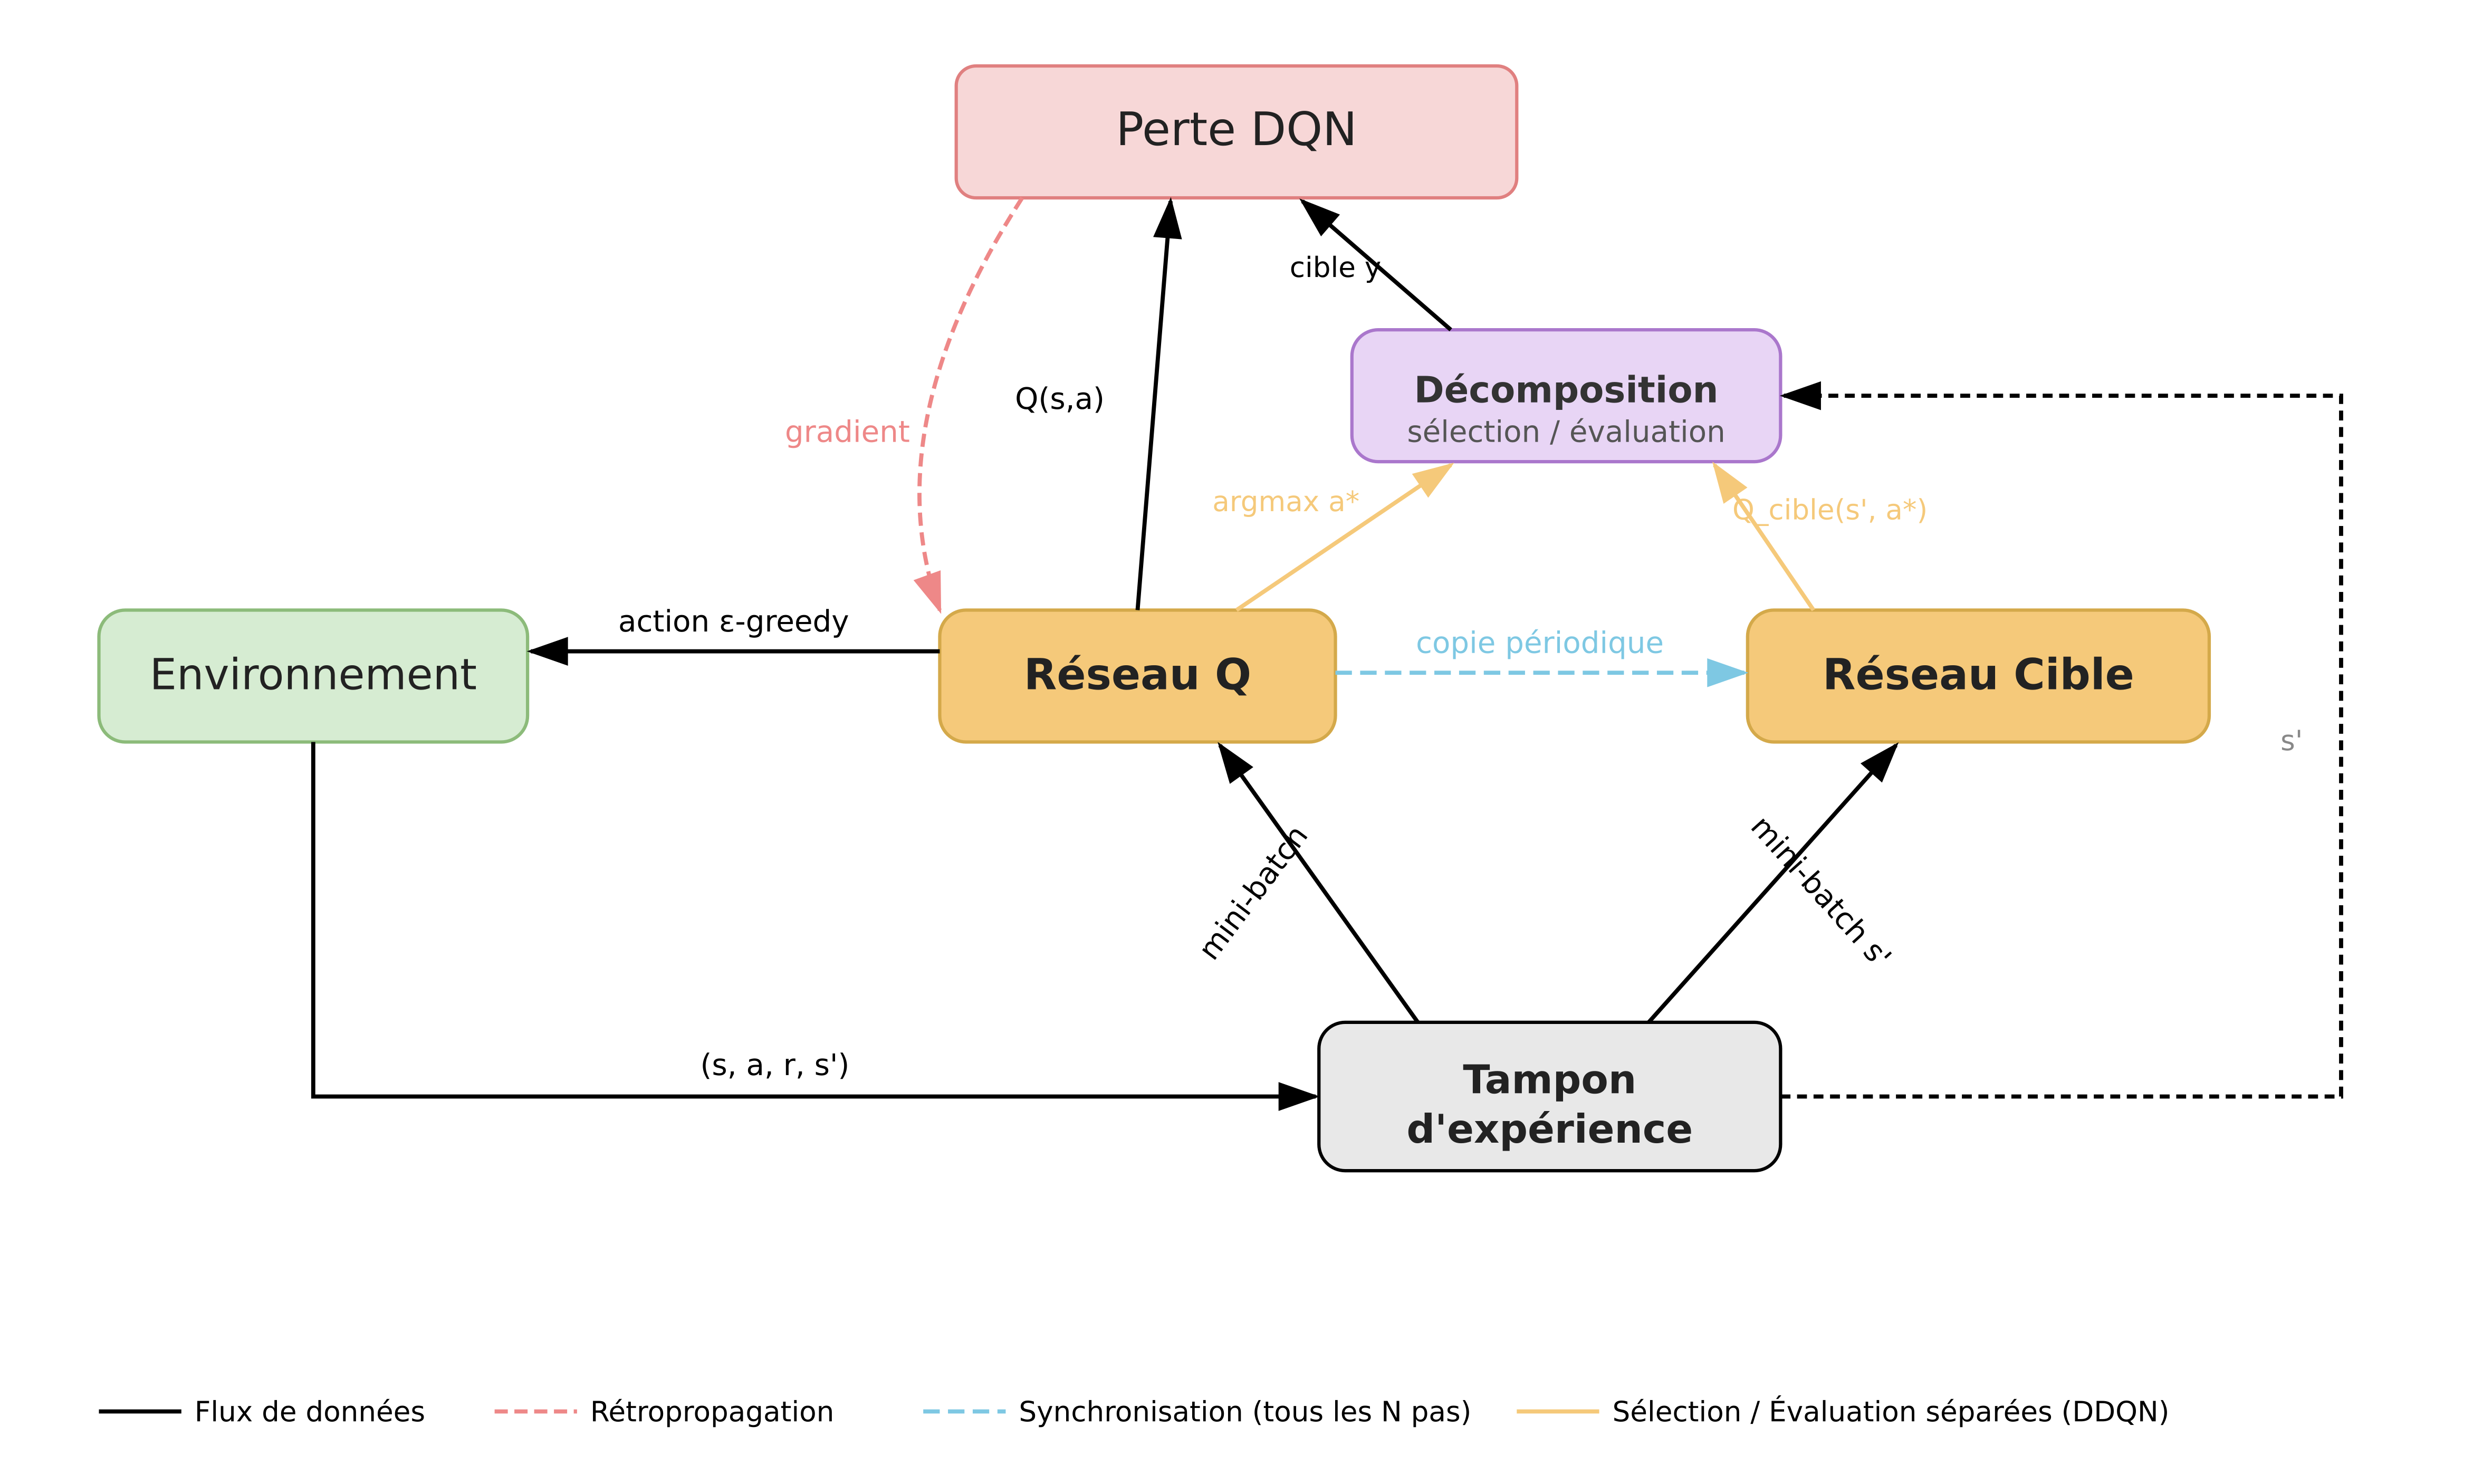
\includegraphics[width=\textwidth]{images/ddqn_architecture.png}
		\caption{Architecture DDQN}
		\label{fig:ddqn}
	\end{subfigure}
	\hfill
	\begin{subfigure}{0.8\textwidth}
		\centering
		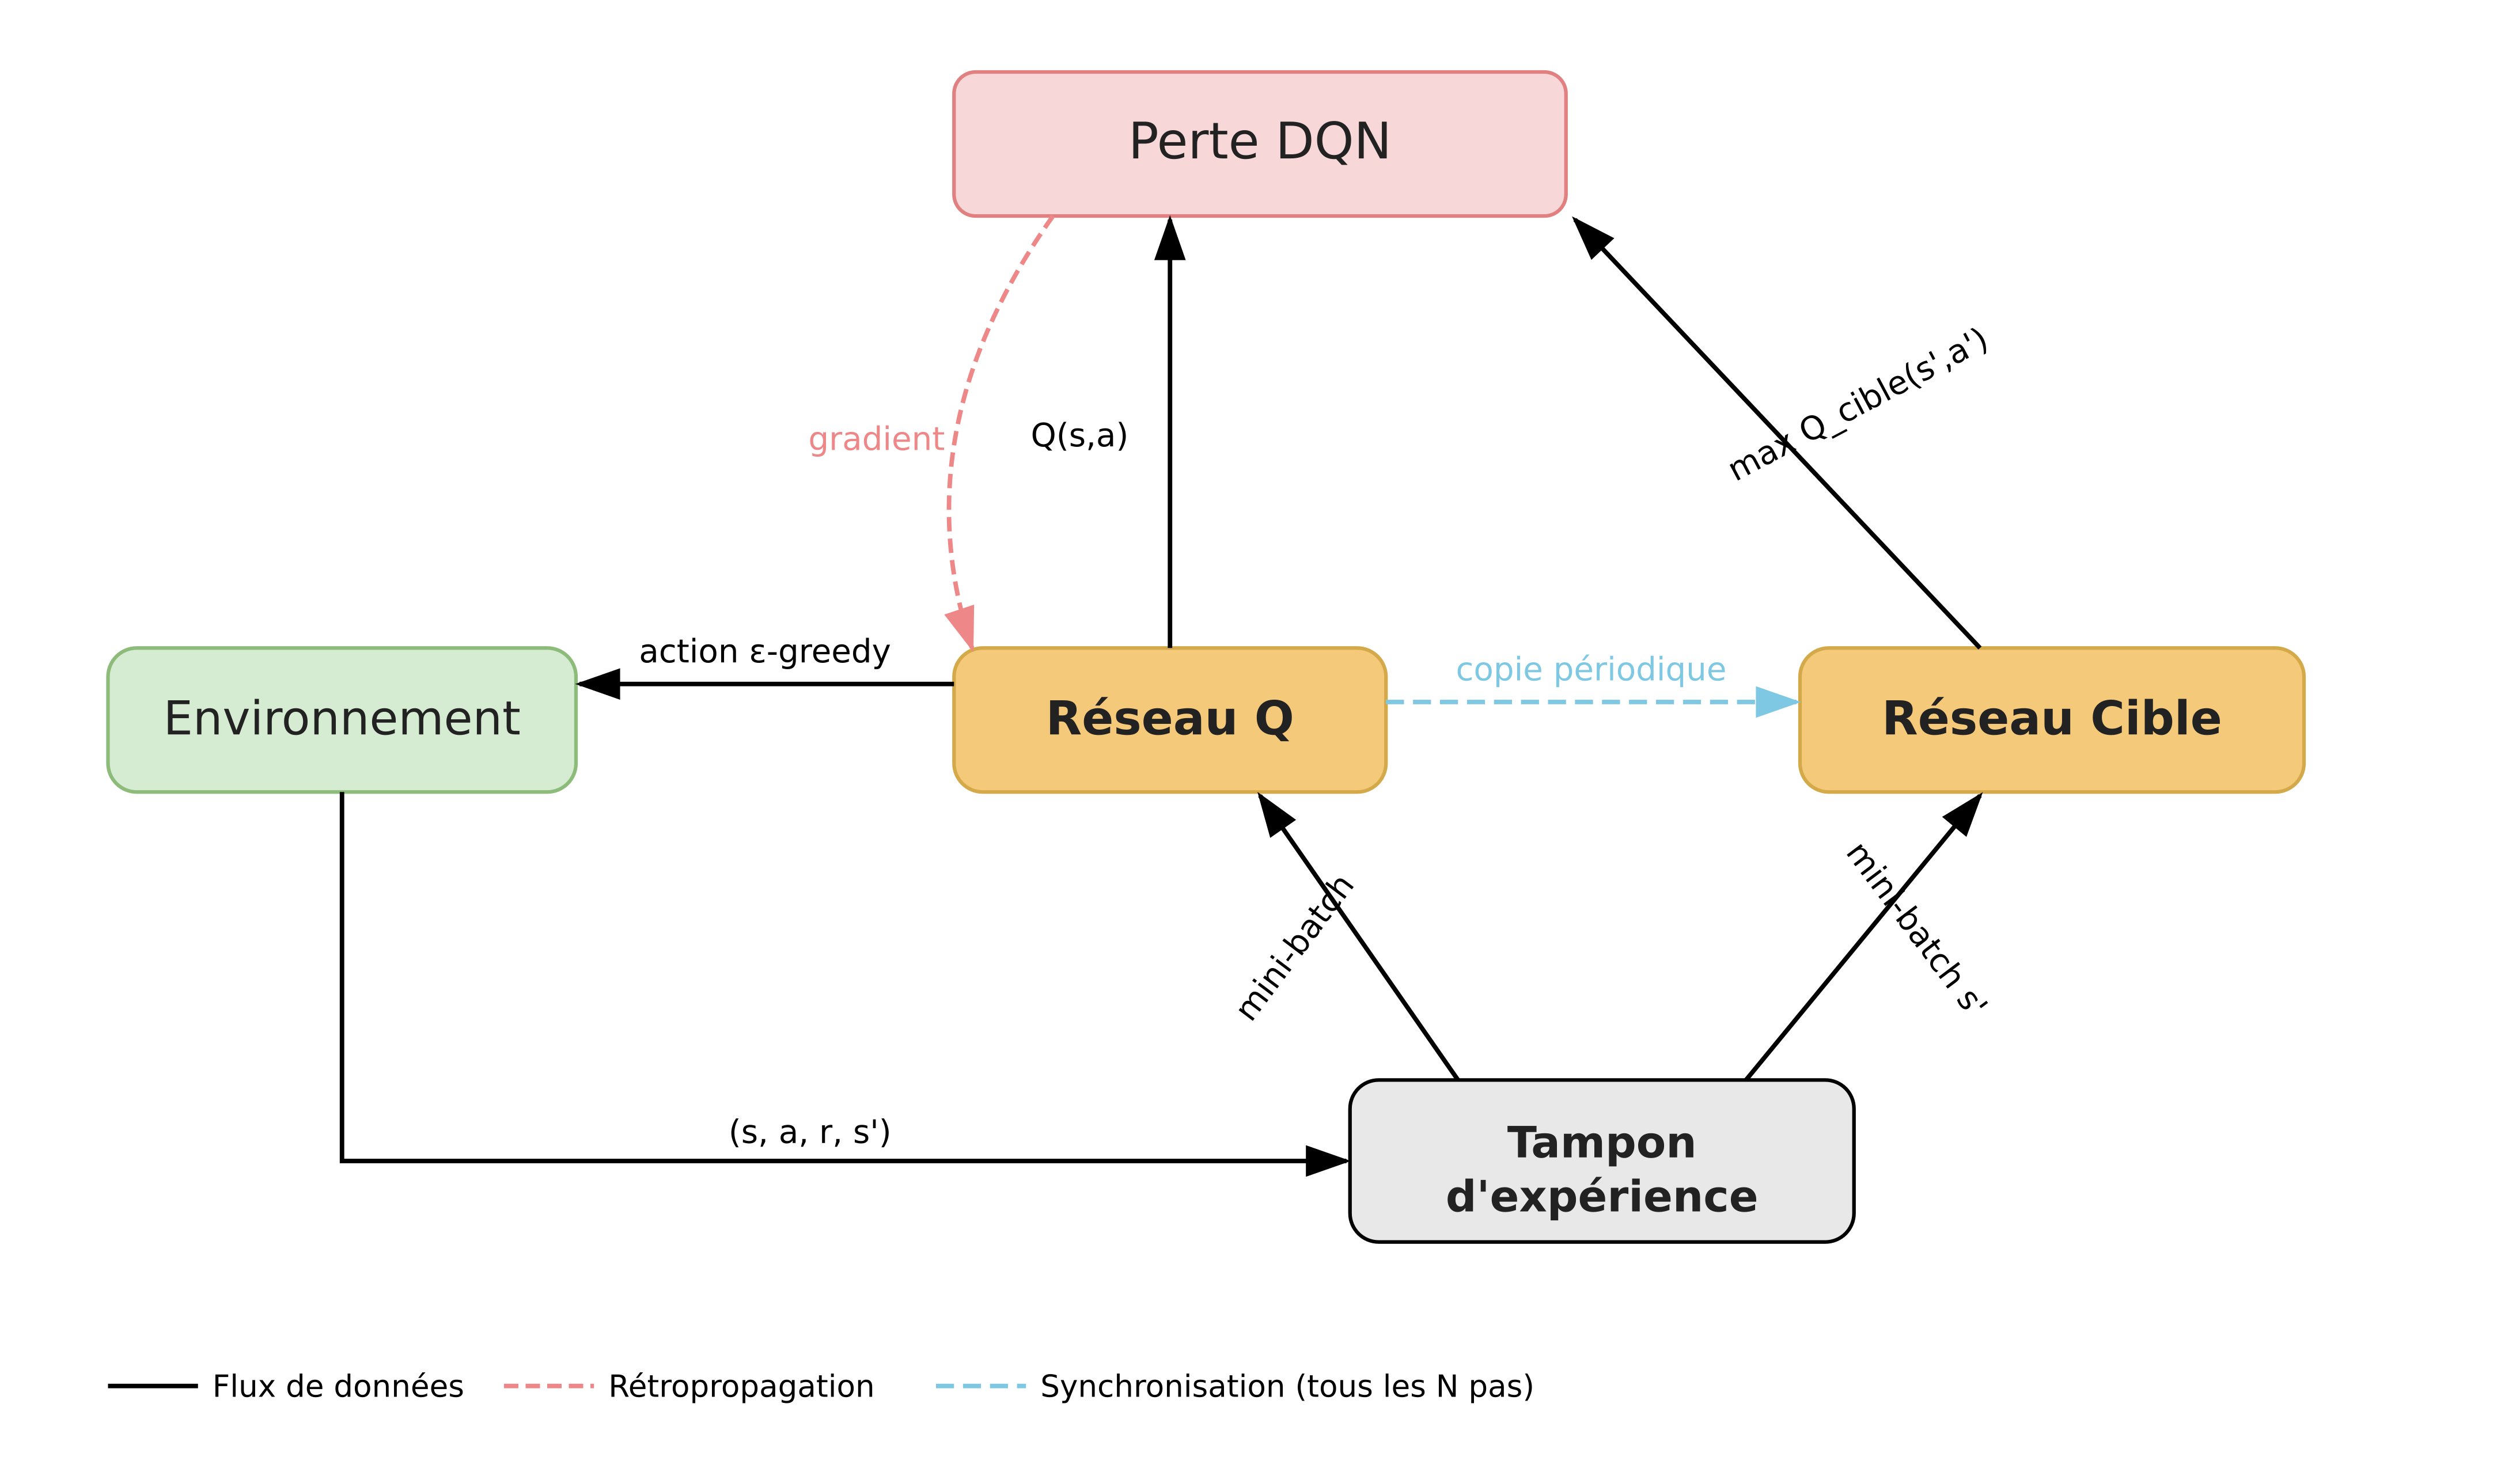
\includegraphics[width=\textwidth]{images/dqn_architecture.png}
		\caption{Architecture DQN}
		\label{fig:dqn}
	\end{subfigure}
	\caption{Comparaison des architectures DQN et DDQN}
	\label{fig:comparaison}
\end{figure}

Cette double estimation, où le réseau principal sélectionne la meilleure action et le réseau cible l'évalue, réduit significativement le biais de surestimation et améliore la stabilité et la rapidité de la convergence.

\clearpage
\subsection{Architecture du réseau de neurones}
\label{subsec:architecture-reseau}

L'architecture repose sur un réseau de neurones multi-couches de type feedforward, conformément à l'approche introduite par \cite{mnih2015dqn}. Celui-ci est composé de deux couches cachées entièrement connectées (128 et 64 neurones) avec fonction d'activation ReLU, choisie pour ses propriétés de convergence rapide et sa capacité à atténuer le problème du gradient évanescent \cite{nair2010relu}. 

Afin de limiter le sur-apprentissage et d'améliorer la capacité de généralisation du modèle, une régularisation par Dropout avec un taux de 0,1 est appliquée après la première couche cachée, suivant la méthodologie proposée par \cite{srivastava2014dropout}. 

La couche de sortie comporte 76 neurones linéaires correspondant aux valeurs $Q(s,a)$ pour chaque action possible. Aucune fonction d'activation n'est utilisée en sortie, conformément à la formulation du Deep Q-Network où les valeurs Q ne sont pas bornées \cite{mnih2015dqn}. 

Les fondements théoriques de l'approximation de fonction en apprentissage par renforcement s'appuient également sur les travaux de référence de \cite{sutton2018rl}.

\begin{figure}[H]
	\centering
	\resizebox{0.95\textwidth}{!}{%
		\begin{tikzpicture}[
			neuron/.style={circle, draw, minimum size=0.6cm, inner sep=0pt, font=\tiny},
			layer/.style={rectangle, draw, minimum width=1.8cm, minimum height=0.7cm, rounded corners, font=\small},
			arrow/.style={->, >=stealth, thick}
			]
			
			% Couche d'entrée (8 neurones)
			\foreach \i in {1,...,8} {
				\node[neuron, fill=blue!20] (input-\i) at (0, -0.7*\i) {};
			}
			\node[below of=input-8, node distance=0.7cm, font=\small] {Entrée (8)};
			
			% Première couche cachée (128 neurones)
			\node[layer, fill=green!20, right=1.6cm of input-4] (hidden1) {Couche 1};
			\node[below of=hidden1, node distance=0.9cm, font=\tiny] {128 neurones};
			
			% Dropout
			\node[layer, fill=yellow!20, right=1.6cm of hidden1] (dropout) {Dropout};
			\node[below of=dropout, node distance=0.9cm, font=\tiny] {p = 0.1};
			
			% Deuxième couche cachée (64 neurones)
			\node[layer, fill=green!20, right=1.6cm of dropout] (hidden2) {Couche 2};
			\node[below of=hidden2, node distance=0.9cm, font=\tiny] {64 neurones};
			
			% Couche de sortie (76 neurones)
			\node[layer, fill=orange!20, right=1.6cm of hidden2] (output) {Sortie};
			\node[below of=output, node distance=0.9cm, font=\tiny] {76 neurones};
			
			% Connexions
			\draw[arrow] (input-4.east) -- node[above, sloped, font=\tiny] {8→128} (hidden1.west);
			\draw[arrow] (hidden1.east) -- (dropout.west);
			\draw[arrow] (dropout.east) -- (hidden2.west);
			\draw[arrow] (hidden2.east) -- (output.west);
			
		\end{tikzpicture}%
	}
	\caption{Architecture du réseau DDQN.}
	\label{fig:ddqn-architecture}
\end{figure}

L'architecture se compose des éléments suivants :
\begin{enumerate}
	\item \textbf{Couche d'entrée} : 8 neurones, correspondant aux 8 dimensions de l'espace d'états.
	\item \textbf{Première couche cachée} : 128 neurones avec une fonction d'activation ReLU (\textit{Rectified Linear Unit}). Cette couche projette l'état dans un espace de dimension supérieure, permettant de capturer des interactions complexes entre les variables d'entrée.
	\item \textbf{Couche de Dropout} : Une couche de régularisation qui désactive aléatoirement 10\% des neurones de la couche précédente pendant l'entraînement. Cela force le réseau à apprendre des représentations redondantes et réduit le risque de sur-apprentissage.
	\item \textbf{Seconde couche cachée} : 64 neurones avec activation ReLU. Elle compresse l'information apprise en une représentation plus compacte.
	\item \textbf{Couche de sortie} : 76 neurones, chacun correspondant à la valeur $Q(s, a)$ estimée pour une action spécifique. Aucune fonction d'activation n'est appliquée en sortie, car les valeurs $Q$ peuvent être négatives.
\end{enumerate}

Cette architecture contient un peu plus de 14 000 paramètres, ce qui permet une inférence en quelques millisecondes sur un processeur standard, rendant l'agent parfaitement adapté à une utilisation en temps réel.

\section{Algorithme et environnement d'entraînement}
\label{sec:algorithme-entrainement}
Cette section décrit l’algorithme d’entraînement de l’agent DDQN et l’environnement
utilisé pour simuler les transmissions LR-FHSS. Elle présente d’abord l’environnement
d’apprentissage et la stratégie d’exploration, puis détaille les mécanismes clés de
l’apprentissage, l’algorithme complet, et enfin l’analyse des hyperparamètres et
de la convergence.

\subsection{Environnement d'apprentissage}
\label{subsec:environnement-sequentiel}

L'entraînement de l'agent s'effectue dans un environnement dédié, \texttt{TrainingEnvironment}, qui simule des épisodes de transmissions. À chaque épisode, les conditions de départ (distance, ombrage) sont tirées aléatoirement selon une distribution réaliste. Cette diversité de situations force l'agent à apprendre une politique généraliste, applicable à n'importe quel nœud du réseau, plutôt qu'une politique sur-optimisée pour un seul scénario.

\begin{figure}[H]
	\centering
	\begin{tikzpicture}[node distance=1.5cm, auto]
		% Début de l'épisode
		\node[rectangle, draw, fill=blue!10, rounded corners] (reset) {Choix de la distance};
		
		% Boucle temporelle
		\node[rectangle, draw, fill=green!10, rounded corners, below of=reset] (action) {Agent choisit $(DR, P_{TX})$};
		\node[rectangle, draw, fill=yellow!10, rounded corners, below of=action] (transmission) {Simulation transmission};
		\node[rectangle, draw, fill=orange!10, rounded corners, below of=transmission] (reward) {Calcul récompense $\mathcal{R}$};
		\node[rectangle, draw, fill=red!10, rounded corners, below of=reward] (transition) {Transition vers $s_{t+1}$};
		
		% Flèches
		\draw[->, thick] (reset) -- (action);
		\draw[->, thick] (action) -- (transmission);
		\draw[->, thick] (transmission) -- (reward);
		\draw[->, thick] (reward) -- (transition);
		\draw[<-, thick] (action.east) -- ++(1,0) node[right] {Fin épisode?} -- ++(0, -4.5) -| (transition.east);
		
		% Conditions de fin
		\node[rectangle, draw, fill=gray!10, dashed, right=2cm of transition] (end) {Si $t \geq T_{\max}$};
		
	\end{tikzpicture}
	\caption{Déroulement d'un épisode dans l'environnement d'entraînement.}
	\label{fig:training-episode}
\end{figure}

Le modèle de propagation et les calculs de \gls{rssi}, \gls{snr}, \gls{ber} ainsi que l'évaluation de la réussite ou de l'échec de la transmission sont assurés par notre simulateur calibré sur l'étude de référence \cite{lrfhss_comparaison}.

\subsection{\texorpdfstring{Stratégie d'exploration : $\epsilon$-greedy}{Stratégie d'exploration : epsilon-greedy}}
\label{subsec:epsilon-greedy}

Pendant l'entraînement, l'agent doit équilibrer deux phases contradictoires : l'exploration, où il essaie de nouvelles actions pour découvrir leurs conséquences, et l'exploitation, où il utilise ses connaissances actuelles pour maximiser la récompense. La stratégie $\epsilon$-greedy est une méthode simple et efficace pour gérer ce compromis.

Avec une probabilité $\epsilon$, l'agent choisit une action aléatoirement (exploration). Avec une probabilité $1-\epsilon$, il choisit l'action qui maximise la valeur $Q$ estimée pour l'état courant (exploitation).

\begin{equation}
	a_t =
	\begin{cases}
		\text{action aléatoire uniforme} & \text{avec probabilité } \epsilon_t \\
		\arg\max_{a} Q_\theta(s_t, a) & \text{avec probabilité } 1 - \epsilon_t
	\end{cases}
\end{equation}

Le paramètre $\epsilon$ n'est pas constant. Il suit une décroissance exponentielle dans le temps :
\begin{equation}
	\epsilon_t = \max(\epsilon_{\text{min}}, \epsilon_{\text{start}} \times \epsilon_{\text{decay}}^t)
\end{equation}
La figure suivante  \ref{fig:epsilon-decay-3000} illustre cette évolution.

\begin{figure}[H]
	\centering
	\begin{tikzpicture}
		\begin{axis}[
			width=14cm, height=6cm,
			xlabel={Épisode},
			ylabel={$\epsilon$},
			grid=both,
			minor tick num=1,
			xtick={0,500,1000,1500,2000,2500,3000},
			ytick={0,0.2,0.4,0.6,0.8,1.0},
			domain=0:3000,
			samples=1000,
			legend style={at={(0.95,0.95)}, anchor=north east, font=\small},
			]
			\addplot[blue, thick] {max(0.01, 1.0 * 0.995^x)};
			\addlegendentry{$\epsilon_t = \max(\epsilon_\text{min}, \epsilon_\text{start} \cdot \epsilon_\text{decay}^t)$}
		\end{axis}
	\end{tikzpicture}
	
	\caption{Évolution du paramètre d'exploration $\epsilon$.}
	\label{fig:epsilon-decay-3000}
\end{figure}

Cette décroissance permet à l'agent d'explorer largement les actions possibles au début, puis de se concentrer progressivement sur l'affinage de la politique apprise.

\subsection{Mécanismes clés de l'apprentissage}
\label{subsec:mecanismes-apprentissage}
Cette sous-section décrit les principaux mécanismes utilisés pour stabiliser et améliorer l’apprentissage de l’agent DDQN. Elle présente d’abord la mémoire d’expérience (Replay Buffer) qui permet de stocker et réutiliser les transitions, puis le rôle des réseaux principal et cible pour assurer une mise à jour stable des valeurs Q.

\subsubsection{Mémoire d’expérience (Replay Buffer)}
L'agent utilise une mémoire d’expérience, notée $\mathcal{D}$, pour stocker ses expériences passées. Chaque expérience est une transition $(s_t, a_t, r_t, s_{t+1}, d_t)$, où $d_t$ indique si l'épisode est terminé. Pendant l'entraînement, l'agent échantillonne aléatoirement un mini-lot (\textit{batch}) de transitions depuis cette mémoire pour mettre à jour son réseau.

Ce mécanisme présente deux avantages majeurs :
\begin{enumerate}
	\item Il brise la corrélation temporelle entre les expériences consécutives, ce qui stabilise l'apprentissage.
	\item Il permet de réutiliser des expériences rares ou anciennes, améliorant l'efficacité d'échantillonnage.
\end{enumerate}

\subsubsection{Réseaux cible et principal}
L'agent maintient deux réseaux de neurones distincts :
\begin{itemize}
	\item Le \textbf{réseau principal} $Q_\theta$, qui est mis à jour à chaque étape par descente de gradient pour minimiser l'erreur de prédiction.
	\item Le \textbf{réseau cible} $Q_{\theta^-}$, qui est une copie du réseau principal mise à jour plus lentement. Il est utilisé pour calculer la valeur cible $y_t$, stabilisant ainsi l'apprentissage.
\end{itemize}

La mise à jour du réseau cible se fait par une mise a jour lente (\textit{soft update}) :
\begin{equation}
	\theta^- \leftarrow \tau \theta + (1 - \tau) \theta^-
\end{equation}
avec $\tau \ll 1$ (typiquement 0,005). Cette mise à jour progressive évite les changements brusques de la cible.

\subsection{Algorithme d'entraînement complet}
\label{subsec:algo-complet}

L'algorithme~\ref{alg:ddqn-training} synthétise l'ensemble du processus d'entraînement de l'agent DDQN.

\begin{algorithm}[H]
	\caption{Entraînement de l'agent DDQN pour l'optimisation LR-FHSS}
	\label{alg:ddqn-training}
	\begin{algorithmic}[1]
		\Require Environnement d'entraînement $E$, nombre d'épisodes $N$
		\Ensure Réseau principal $Q_\theta$ (politique apprise)
		
		\State Initialiser le réseau principal $Q_\theta$ avec des poids aléatoires
		\State Initialiser le réseau cible $Q_{\theta^-}$ avec les mêmes poids que $Q_\theta$
		\State Initialiser la mémoire de replay $\mathcal{D}$ (capacité $C = 10 000$)
		\State Initialiser le paramètre d'exploration $\epsilon \leftarrow 1.0$
		
		\For{épisode $e = 1$ à $N$}
		\State $s \gets E.\text{reset}()$ \Comment{Nouvel épisode, nouvel état initial}
		\State $R_{\text{total}} \gets 0$
		
		\While{l'épisode n'est pas terminé}
		\State $a \gets$ sélectionner action avec $\epsilon$-greedy à partir de $Q_\theta(s)$
		\State $(r, s', d) \gets E.\text{step}(a)$ \Comment{Exécuter l'action dans l'environnement}
		\State Stocker $(s, a, r, s', d)$ dans $\mathcal{D}$
		\State $R_{\text{total}} \gets R_{\text{total}} + r$
		
		\If{$|\mathcal{D}| \geq$ batch\_size}
		\State Échantillonner un mini-lot $\mathcal{B}$ de transitions depuis $\mathcal{D}$
		\State Calculer les valeurs cibles $y$ pour chaque transition de $\mathcal{B}$ (équation DDQN)
		\State Mettre à jour $Q_\theta$ par descente de gradient sur la perte $\mathcal{L} = \frac{1}{|\mathcal{B}|}\sum (Q_\theta(s,a) - y)^2$
		\State Mettre à jour le réseau cible : $\theta^- \leftarrow \tau \theta + (1 - \tau) \theta^-$
		\EndIf
		
		\State $s \gets s'$
		\EndWhile
		
		\State $\epsilon \gets \max(\epsilon_{\text{min}}, \epsilon \times \epsilon_{\text{decay}})$
		\State Journaliser les métriques de l'épisode ($R_{\text{total}}$, taux de succès, etc.)
		\EndFor
		
		\State \Return $Q_\theta$
	\end{algorithmic}
\end{algorithm}

\subsection{Hyperparamètres et courbes d'apprentissage}
Cette sous-section présente d’abord la configuration des hyperparamètres utilisés pour l’entraînement de l’agent DDQN, puis analyse la convergence du modèle à travers les courbes de récompense, de taux de succès et de perte, illustrant la stabilité et l’efficacité de l’apprentissage.
\subsubsection{Configuration des hyperparamètres}
Le tableau suivant présente les hyperparamètres utilisés pour l'entraînement de notre modèle DDQN.
\begin{table}[H] 
	\centering
	\caption{Hyperparamètres de l'apprentissage DDQN}
	\label{tab:hyperparameters}
	\begin{tabular}{|l|c|l|}
		\hline
		\textbf{Hyperparamètre} & \textbf{Valeur} & \textbf{Description} \\
		\hline
		\multicolumn{3}{|c|}{\textbf{Paramètres du réseau}} \\
		\hline
		Taux d'apprentissage ($\alpha$) & $10^{-4}$ & Pas de mise à jour du réseau \\
		Facteur d'actualisation ($\gamma$) & 0,99 & Importance des récompenses futures \\
		Taille du batch & 64 & Nombre d'expériences par apprentissage \\
		\hline
		\multicolumn{3}{|c|}{\textbf{Mémoire et exploration}} \\
		\hline
		Taille du replay buffer & 10 000 & Capacité maximale de mémoire \\
		$\epsilon_{initial}$ & 1 & Probabilité d'exploration initiale \\
		$\epsilon_{final}$ & 0,05 & Probabilité d'exploration minimale \\
		Décroissance d'$\epsilon$ & 0,995 & Facteur de réduction par épisode \\
		\hline
		\multicolumn{3}{|c|}{\textbf{Synchronisation}} \\
		\hline
		Fréquence mise à jour cible & 100 pas & Pas entre synchronisations \\
		$\tau$ (soft update) & 0,001 & Taux de mise à jour progressive \\
		\hline
		\multicolumn{3}{|c|}{\textbf{Environnement}} \\
		\hline
		Nombre d'épisodes & 3000 & Durée totale d'entraînement \\
		Pas par épisode & 100 & Interactions par épisode \\
		\hline
	\end{tabular}
\end{table}	

\subsubsection{Analyse de la convergence}

La figure \ref{fig:reward} illustre la progression de l'apprentissage avec une forte variance initiale (épisodes 1-100) où les récompenses fluctuent entre -12431 et +6979, caractéristique d'une phase d'exploration intensive visible dans la figure \ref{fig:epsilon}. Une convergence progressive s'opère à partir de 450 épisodes, avec une récompense moyenne stabilisée autour de 6870 ± 2150 sur les 500 derniers épisodes.

Le taux de succès (Fig. \ref{fig:success}) atteint 89\% en moyenne en fin d'entraînement, avec des pics réguliers à 100\% dès l'épisode 6 et des séquences soutenues de réussite complète (notamment aux épisodes 920-935), démontrant l'efficacité de l'approche proposée.

L'évolution de la fonction de perte (Fig. \ref{fig:loss}) confirme un apprentissage stable du réseau : après une augmentation initiale traduisant l'acquisition des connaissances, la perte se stabilise autour de 198 ± 8 à partir de 1000 épisodes, indiquant une convergence satisfaisante.

\begin{figure}[H]
	\centering
	\begin{subfigure}[b]{0.48\textwidth}
		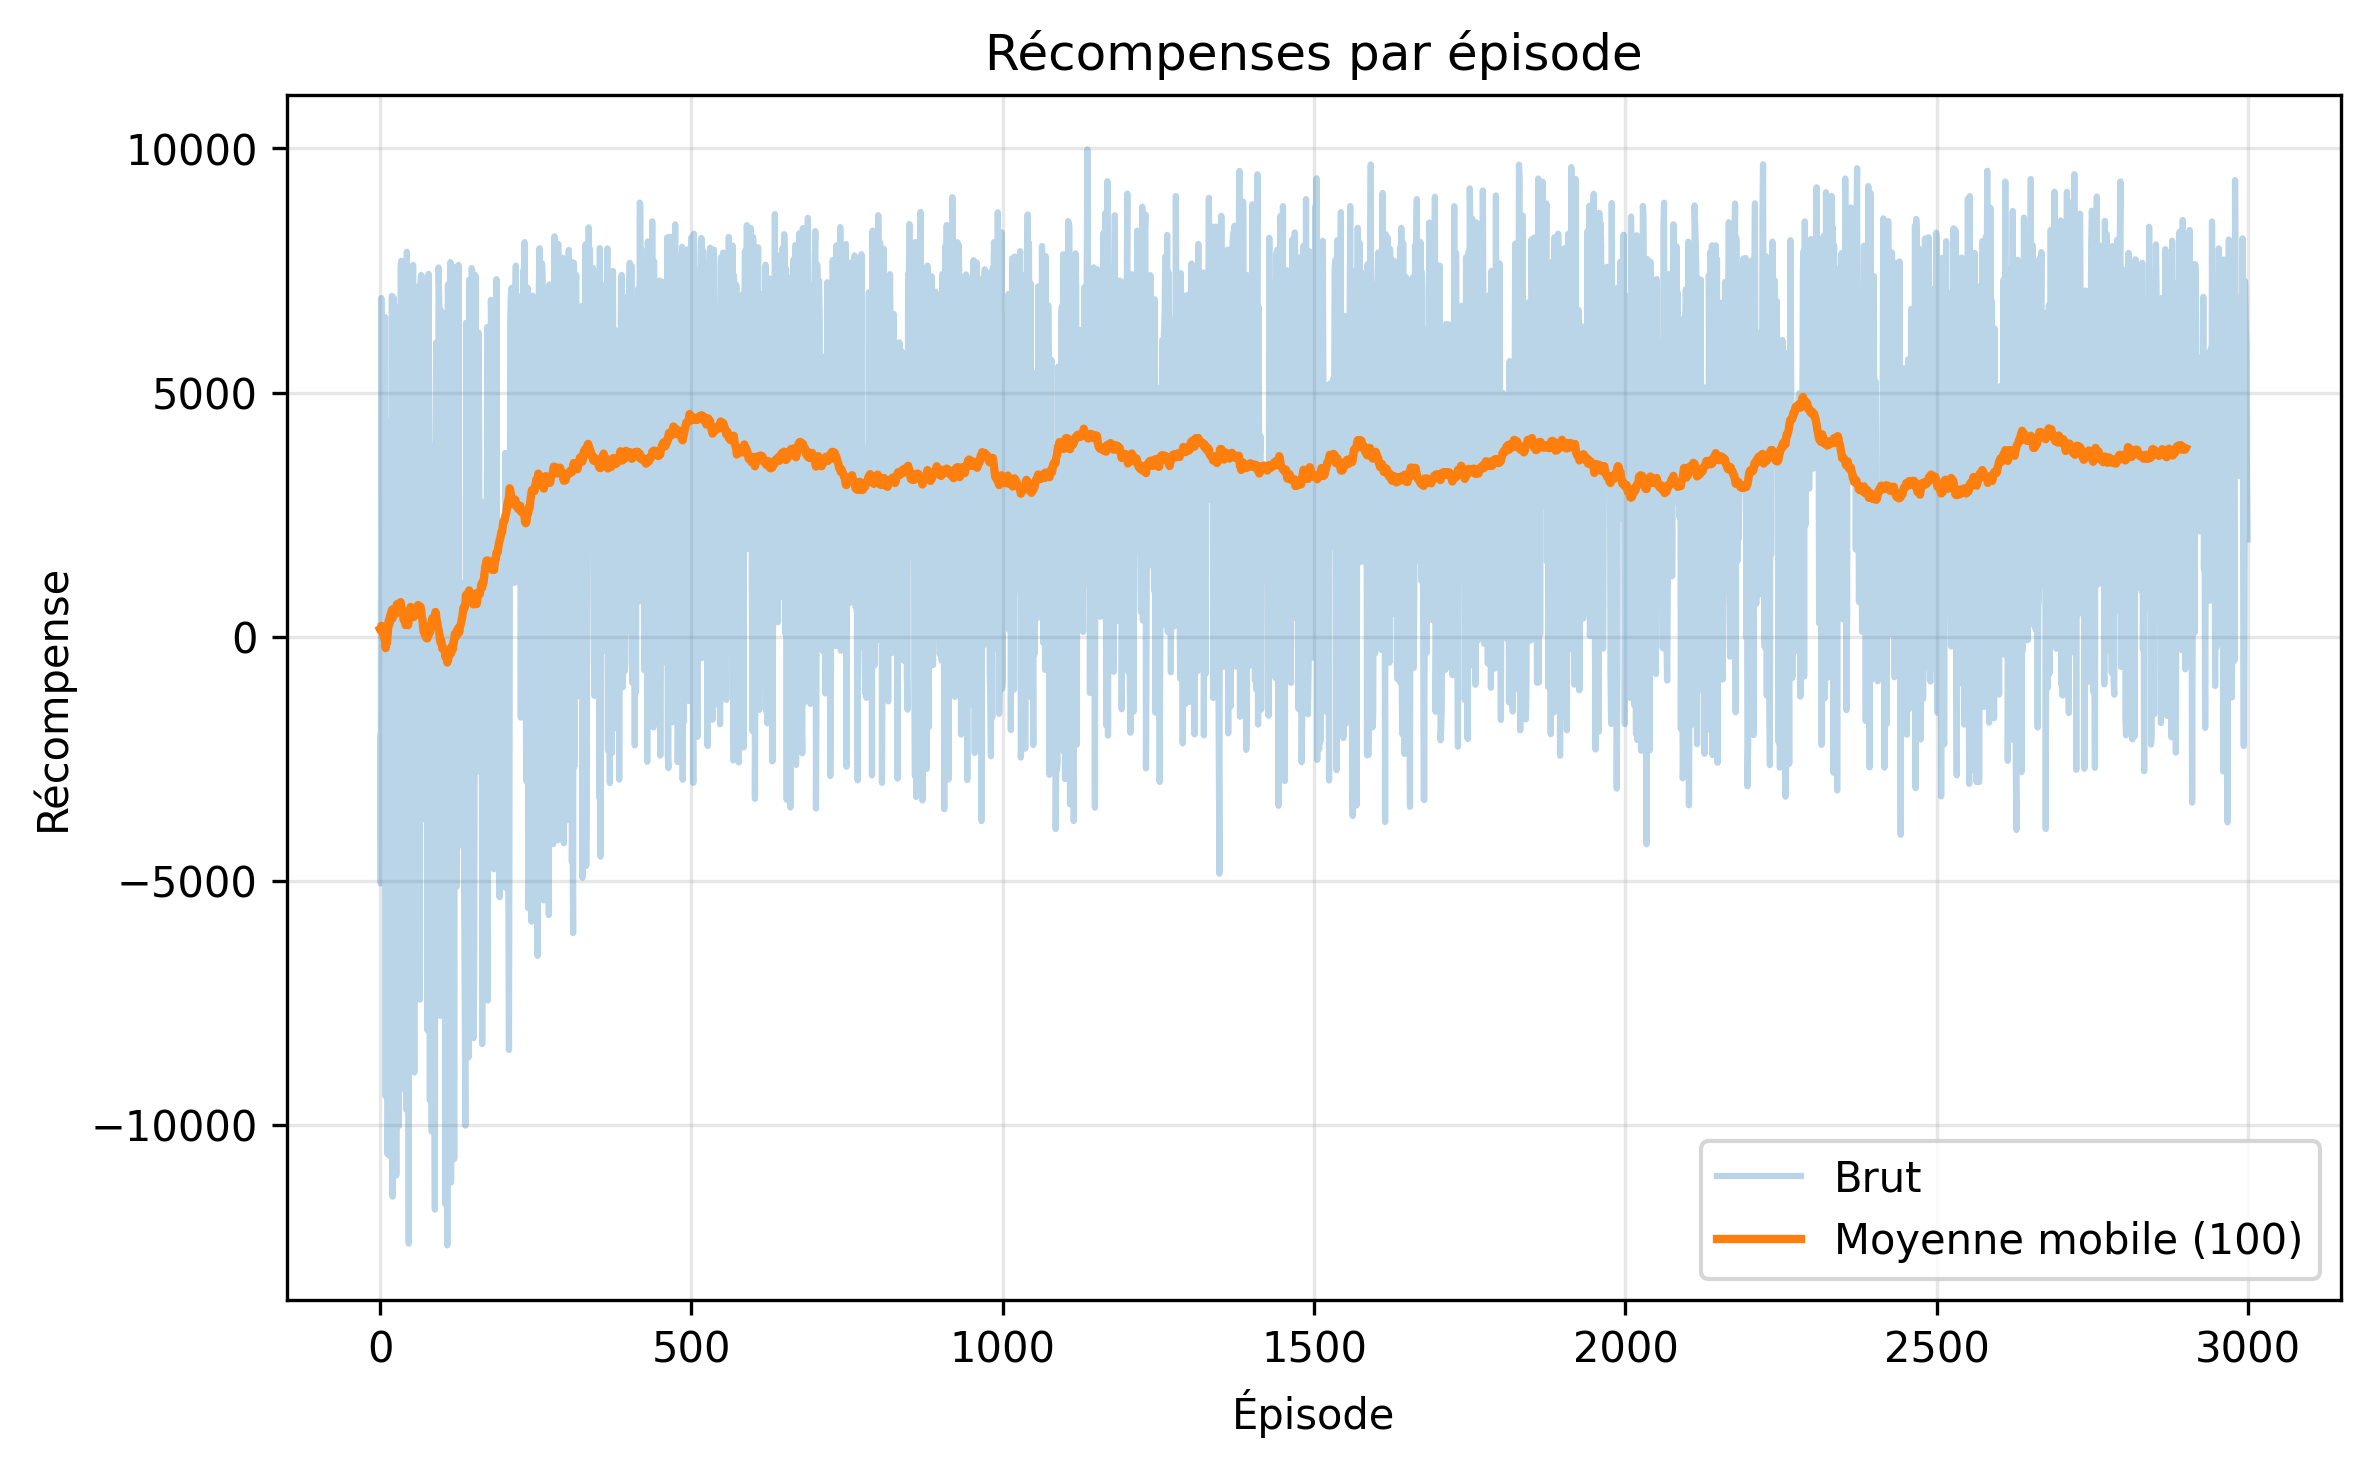
\includegraphics[width=\textwidth]{images/validation/training/01_recompenses.png}
		\caption{Récompense cumulée par épisode}
		\label{fig:reward}
	\end{subfigure}
	\hfill
	\begin{subfigure}[b]{0.48\textwidth}
		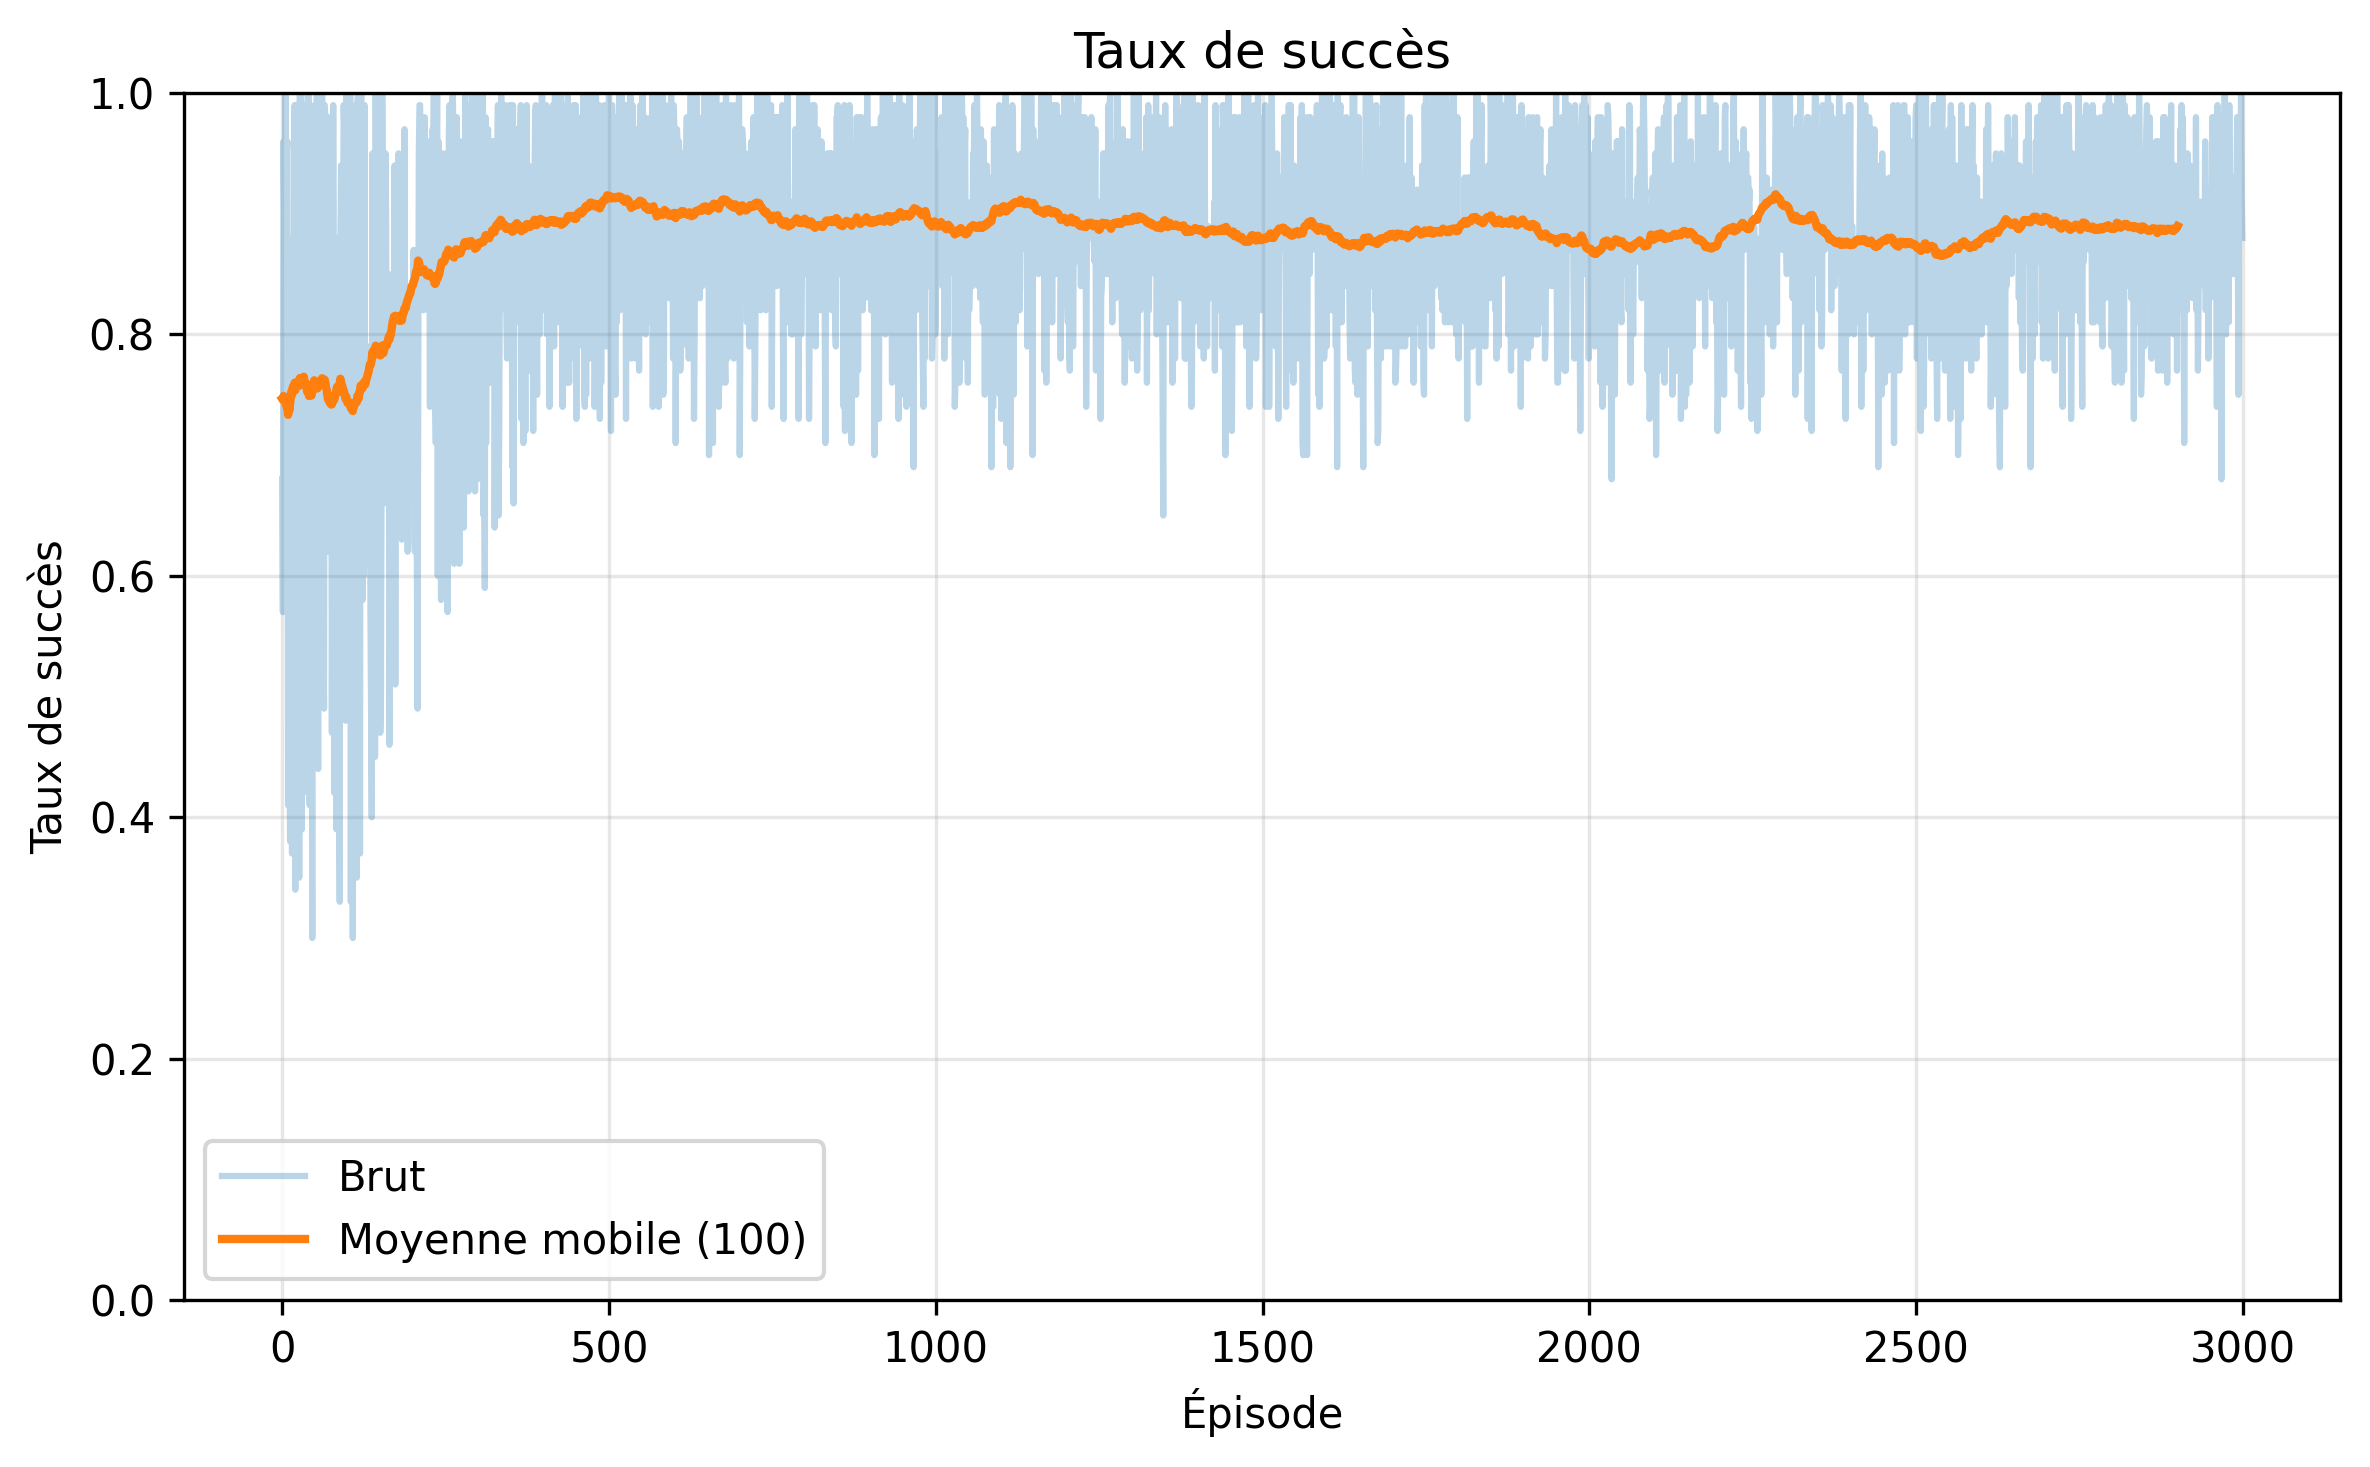
\includegraphics[width=\textwidth]{images/validation/training/02_taux_succes.png}
		\caption{Taux de succès des paquets}
		\label{fig:success}
	\end{subfigure}
	
	\vspace{0.3cm}
	
	\begin{subfigure}[b]{0.48\textwidth} 
		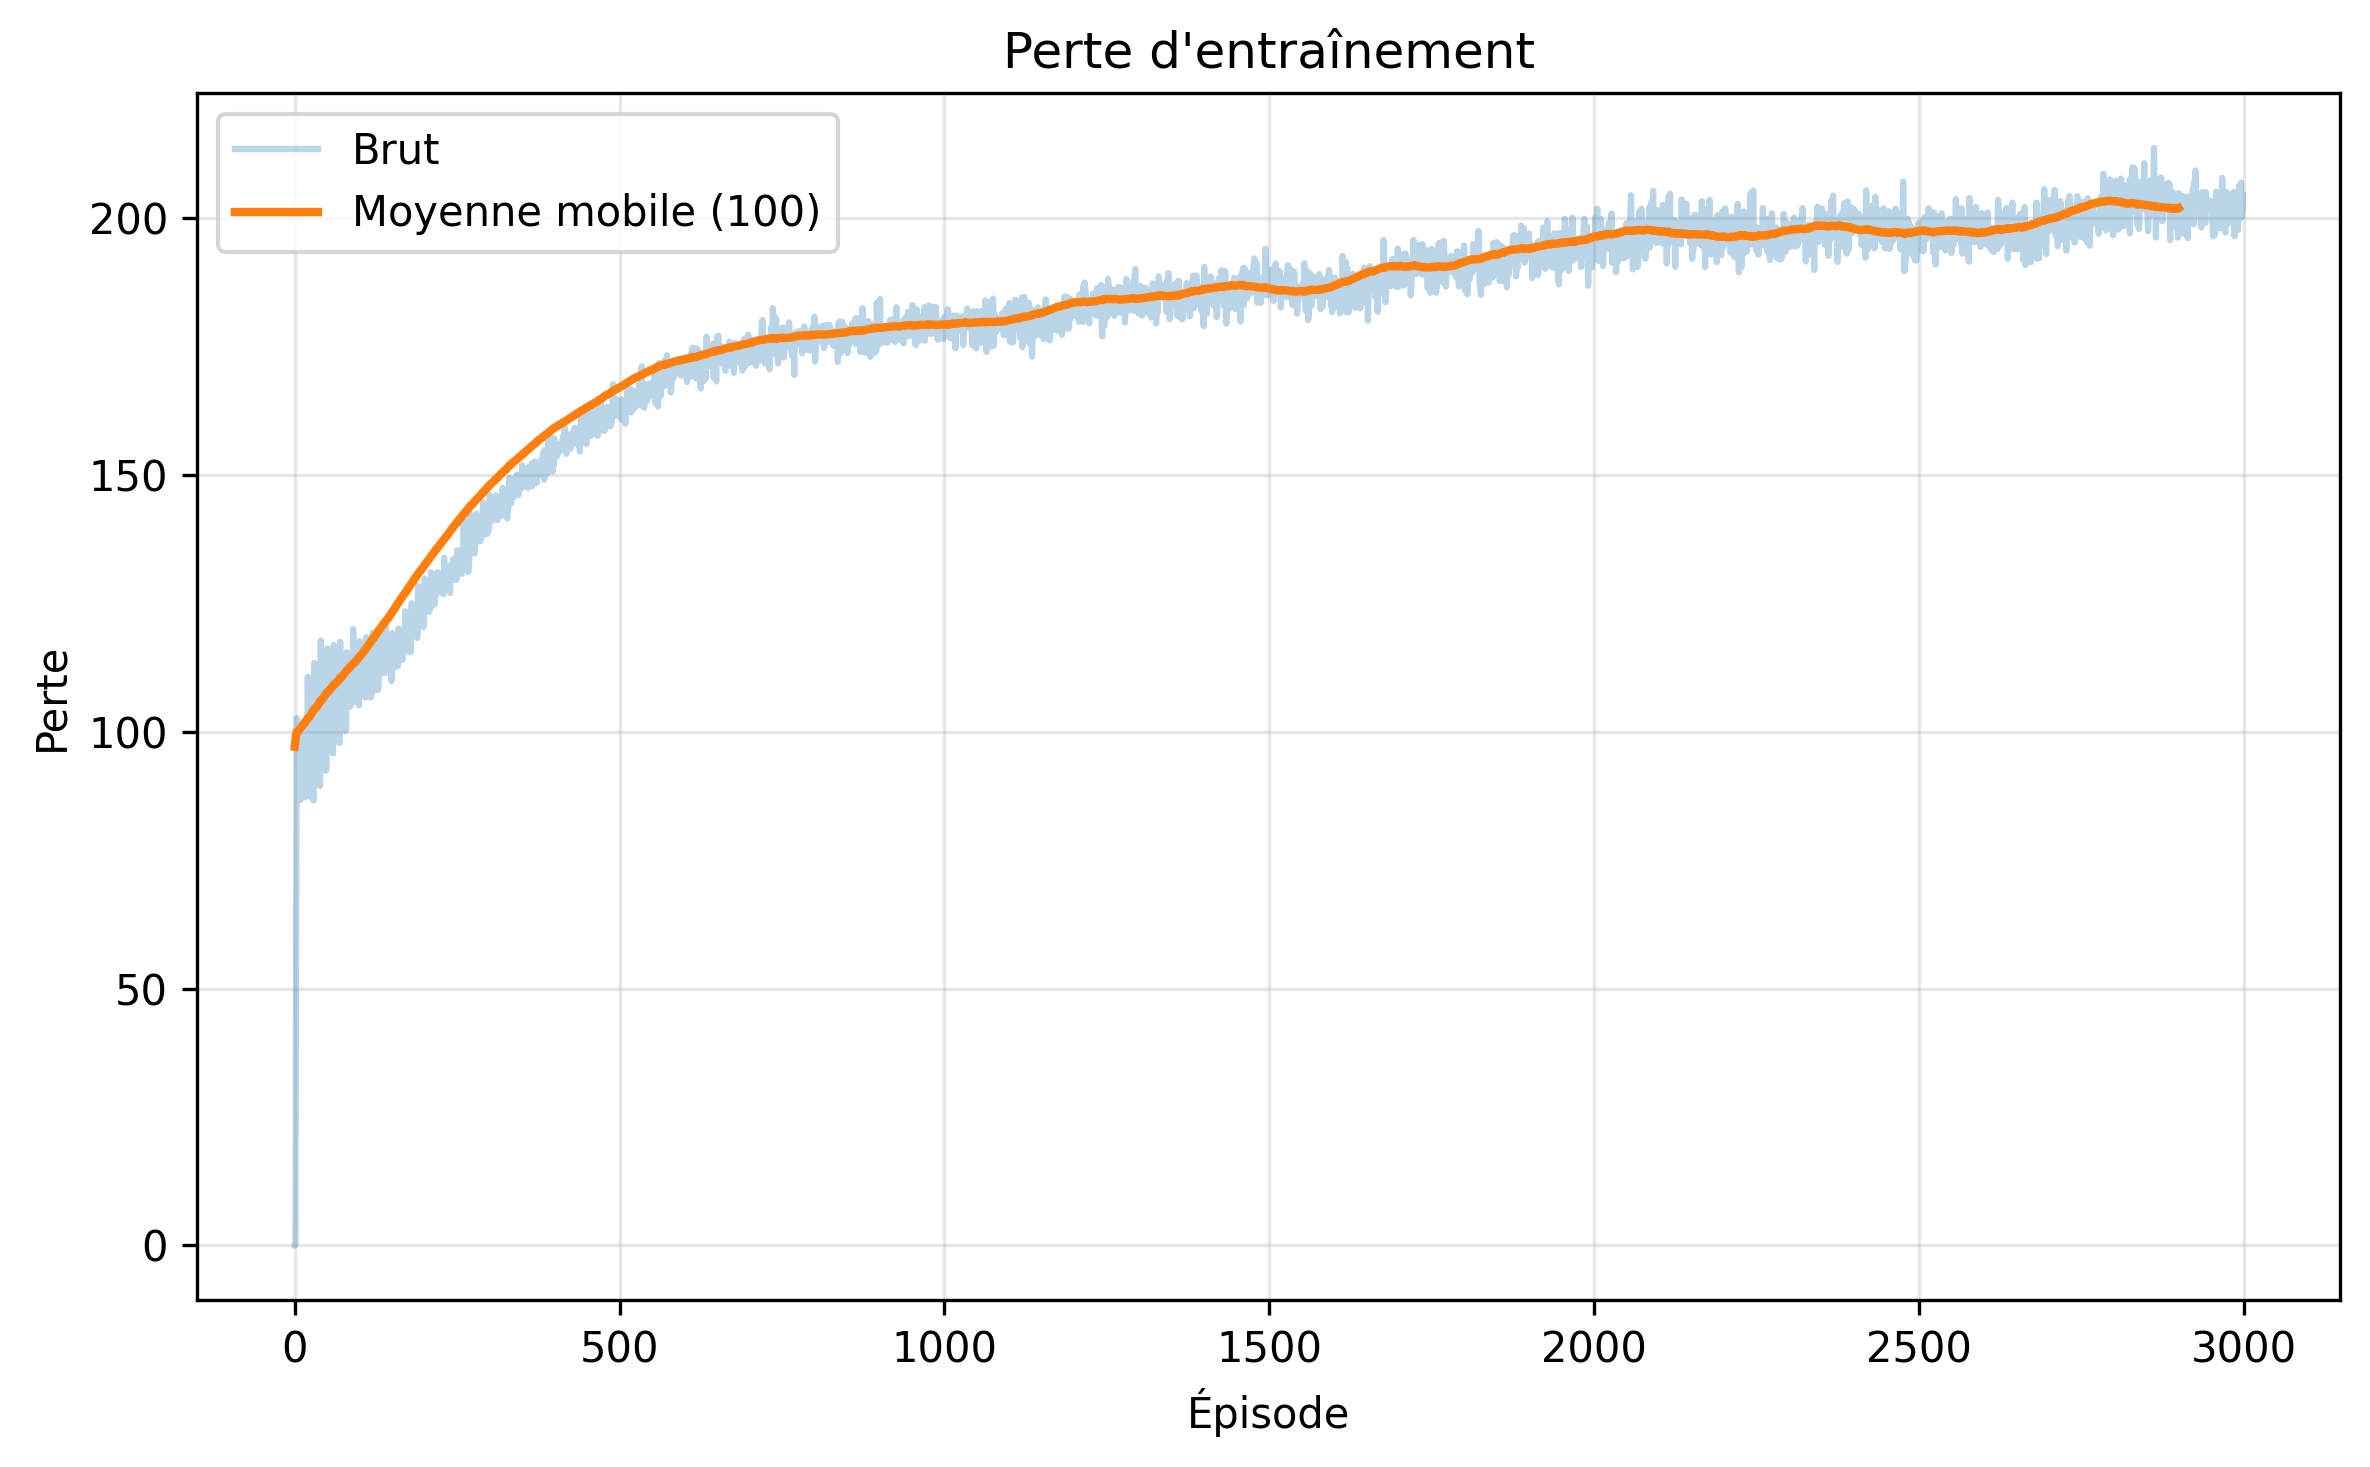
\includegraphics[width=\textwidth]{images/validation/training/03_perte_entrainement.png}
		\caption{Évolution de la fonction de perte}
		\label{fig:loss}
	\end{subfigure}
	\hfill
	\begin{subfigure}[b]{0.48\textwidth}
		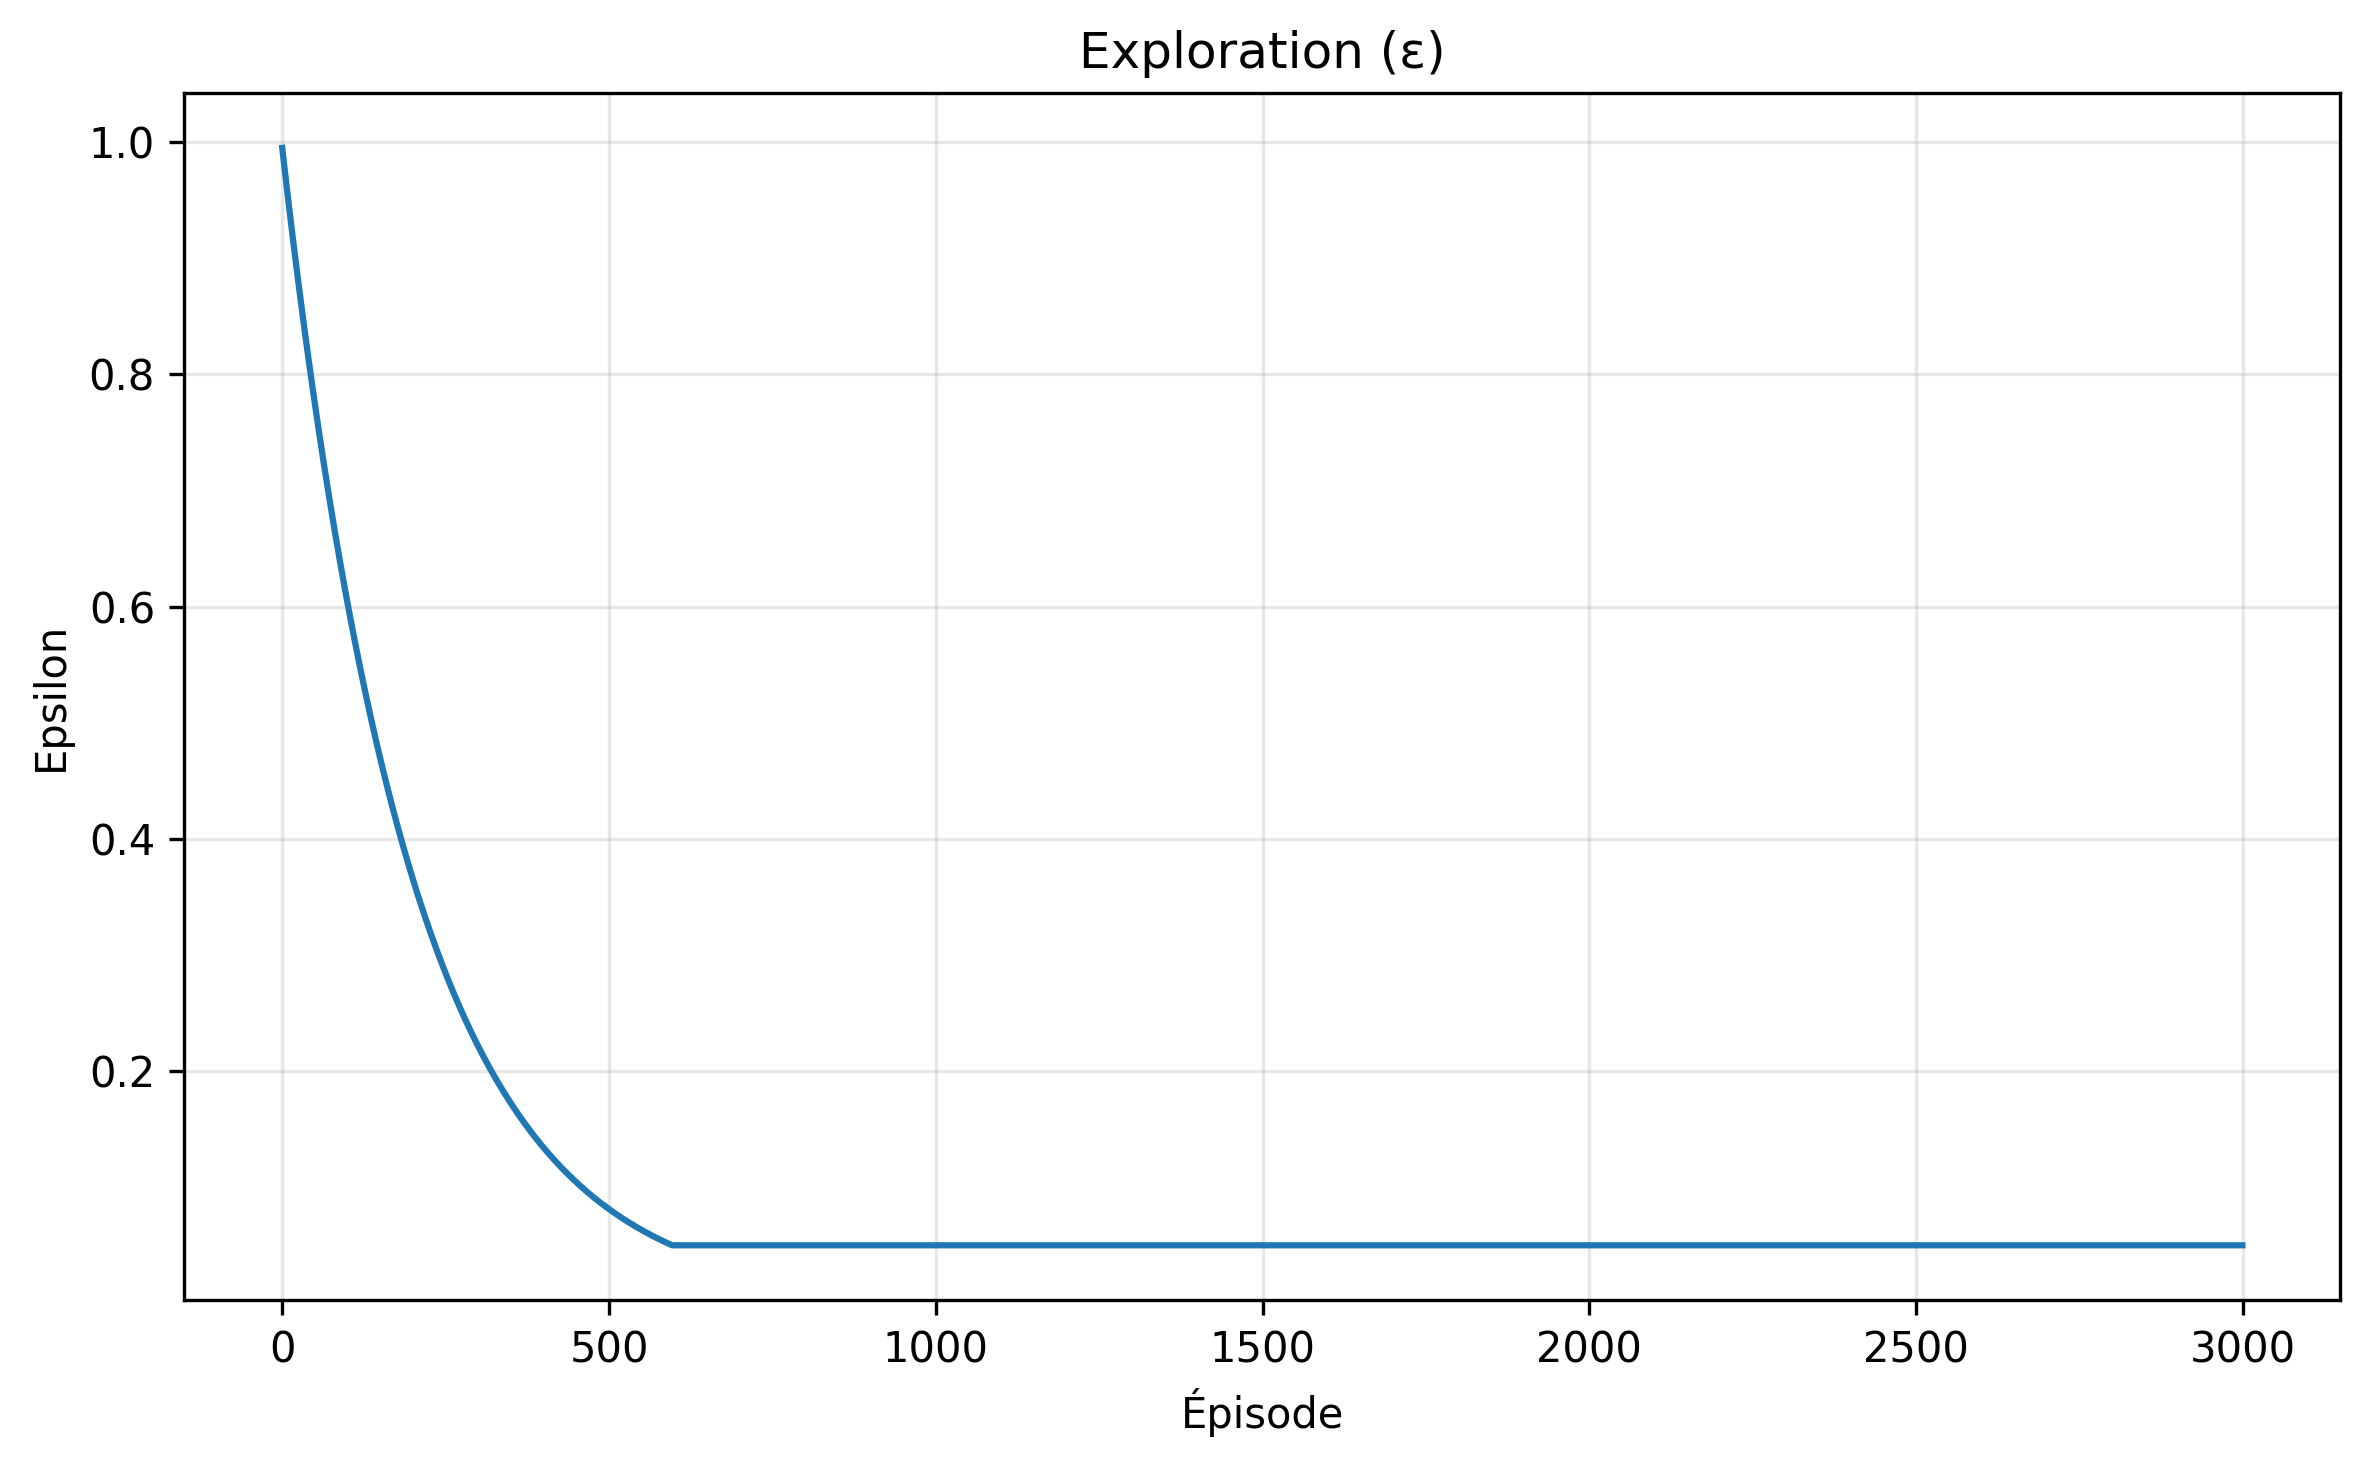
\includegraphics[width=\textwidth]{images/validation/training/05_epsilon.png}
		\caption{Décroissance de la stratégie $\epsilon$-greedy}
		\label{fig:epsilon}
	\end{subfigure}
	\caption{Courbes d'apprentissage de l'agent DDQN}
	\label{fig:training_curves}
\end{figure}


\section{Conclusion}
\label{sec:conclusion-ddqn}

Ce chapitre a posé les fondations théoriques et pratiques de notre approche d'optimisation par apprentissage par renforcement pour les réseaux LR-FHSS. En formulant le problème comme un processus de décision markovien, nous avons défini un cadre pour l'apprentissage d'une politique de transmission adaptative. Le chapitre suivant est entièrement dédié à l'évaluation expérimentale de cette solution.
	\chapter{ÉVALUATION DE LA SOLUTION}

\section{Introduction}
\label{sec:intro-evaluation}

Dans ce chapitre, nous évaluerons notre solution dans des scénarios expérimentaux. Auparavant, nous présenterons notre simulateur LR-FHSS développé et le confronterons à des mesures réelles pour sa validation. Ensuite, nous exposerons les forces et limites de notre modèle DDQN. En conclusion, nous évoquerons les perspectives futures d'amélioration.

\section{Outil de simulation développé}
\label{sec:outil-simulation}

Pour mener à bien l'évaluation de notre solution, nous avons développé un simulateur événementiel en Python, constituant la plateforme expérimentale centrale pour l'analyse des performances de LR-FHSS.

\subsection{Architecture et composants fondamentaux}

	Le simulateur est basé sur une boucle événementielle permettant de représenter précisément les transmissions asynchrones et les conflits d'accès au canal dans un réseau dense. Au cœur du système se trouve la classe \texttt{LR\_FHSS\_Simulation}, qui gère une file prioritaire d'événements triés par leur date d'exécution. Cette approche offre plusieurs avantages :
	
	\begin{itemize}
		\item \textbf{Fidélité temporelle} : Le temps de simulation progresse de manière discrète, de la date d'un événement à la suivante. Ce fonctionnement est bien adapté aux transmissions radio, qui sont brèves et ponctuelles.
		
		\item \textbf{Efficacité computationnelle} : Seuls les moments où l'état du système change sont simulés, permettant d'explorer de longues durées avec un grand nombre de nœuds.
	\end{itemize}

Les transmissions sont modélisées par deux structures de données principales, reflétant la structure de trame LR-FHSS : \texttt{SimulatedPacket} qui encapsule toutes les caractéristiques d'une transmission de paquet, et \texttt{TransmissionFragment} qui stocke les paramètres spécifiques à chaque fragment (fréquence exacte, type, bande passante instantanée), permettant une détection précise des collisions au niveau fragment.

\subsection{Modélisation du canal de propagation}

La fidélité du simulateur repose sur la justesse de son modèle de canal. Notre implémentation intègre un modèle de propagation réaliste :

\begin{itemize}
	\item \textbf{Affaiblissement de parcours} : Calculé selon le modèle logarithmique standard largement utilisé dans les études comme \cite{rappaport2002wireless,gonzalez2023lorawan} :
	
	\begin{equation}
		PL(d) = PL(d_0) + 10 n \log_{10}\left(\frac{d}{d_0}\right) + X_\sigma
		\label{eq:path_loss}
	\end{equation}
	
	où \(PL(d)\) est l'affaiblissement de parcours à la distance \(d\) (en dB), \(d_0 = 1\ km\) la distance de référence, \(n = 3,3\) l'exposant d'affaiblissement pour un environnement suburbain/rural par défaut, et \(PL(d_0) = 125\ dB\) l'affaiblissement de référence pour la bande EU868, également proche de la moyenne de la perte à cette distance dans l'article \cite{lrfhss_comparaison}.
	
	\item \textbf{Ombrage (shadowing)} : Modélisé de manière déterministe via un hachage de la position \((x, y)\) et de l'identifiant du nœud, générant une valeur suivant une loi normale :
	
	\begin{equation}
		X_{\sigma} \sim \mathcal{N}(0, \sigma_s^2)
		\label{eq:shadowing}
	\end{equation}
	
	avec \(\sigma_s = 7,0\ dB\) l'écart-type de l'ombrage. Ce mécanisme, illustré par la figure \ref{fig:shadowing_model}, garantit qu'une même position produit toujours la même valeur de \textit{shadowing}, essentiel pour la reproductibilité.
	
	\item \textbf{Calcul du RSSI et SNR} : Le RSSI, qui est la puissance reçue par la passerelle, est obtenu par :
	
	\begin{equation}
		RSSI = P_{tx} - PL(d)
		\label{eq:rssi}
	\end{equation}
	
	où \(P_{tx}\) est la puissance d'émission (dBm). Le SNR est calculé par :
	
	\begin{equation}
		SNR = RSSI - P_{bruit}
		\label{eq:snr}
	\end{equation}
	
	\item \textbf{Puissance de bruit du récepteur}
	
	La puissance de bruit \(P_{bruit}\) (dBm) intègre deux éléments fondamentaux :
	
	\begin{equation}
		P_{bruit} = \underbrace{(-174 + 10 \log_{10}(B))}_{\text{Bruit thermique à 290 K}} + \underbrace{NF}_{\text{Facteur de bruit}}
		\label{eq:bruit_total}
	\end{equation}
	
	Le terme \(-174\ dBm/Hz\) représente la densité spectrale de bruit thermique, résultat fondamental de la physique statistique établi par Nyquist et Johnson \cite{nyquist_1928, johnson_1928}. Pour une température de référence \(T_0 = 290\ K\), le bruit thermique dans une bande \(B\) (Hz) s'exprime par \(k \cdot T \cdot B\) où \(k = 1,38 \times 10^{-23}\ J/K\) est la constante de Boltzmann \cite{boltzmann_1964}.
	
	Le facteur de bruit \(NF\) quantifie la dégradation du SNR due aux différents étages de traitement du récepteur \cite{friis_1944}. Pour les récepteurs LoRa/LR-FHSS, une valeur \(NF = 6,0\ dB\) est représentative \cite{semtech2022lrfhss, Semtech_LR1121_Datasheet_2023}.
	
	Le tableau \ref{tab:bruit_dr} présente les puissances de bruit calculées pour chaque débit de données selon le standard LoRaWAN EU868 \cite{loraalliance2025regional} :
	
	\begin{table}[H]
		\centering
		\caption{Puissance de bruit par débit de données (NF = 6,0 dB)}
		\label{tab:bruit_dr}
		\begin{tabular}{|c|c|c|c|}
			\hline
			\textbf{DR} & \textbf{Bande (kHz)} & \(\mathbf{10\log_{10}(B)}\) & \(\mathbf{P_{bruit}}\) \textbf{(dBm)} \\
			\hline
			DR8/DR9 & 137 & 51,4 & -116,6 \\
			DR10/DR11 & 336 & 55,3 & -112,7 \\
			\hline
		\end{tabular}
	\end{table}
	
	Ces valeurs constituent la référence pour le calcul du SNR à partir des mesures de RSSI selon l'équation \ref{eq:snr}.
	
	\begin{figure}[!h]
		\centering
		\begin{tikzpicture}
			\begin{axis}[
				width=12cm,
				height=7cm,
				domain=-25:25,
				samples=200,
				axis lines=middle,
				xlabel={$X_\sigma$ (dB)},
				ylabel={Densité de probabilité},
				ymin=0,
				ymax=0.08,
				xtick={-21,-14,-7,0,7,14,21},
				xticklabels={$-3\sigma_s$,$-2\sigma_s$,$-\sigma_s$,0,$\sigma_s$,$2\sigma_s$,$3\sigma_s$},
				ytick=\empty,
				enlargelimits=true,
				grid=both,
				grid style={dashed,gray!30}
				]
				
				% Gaussian curve (sigma = 7 dB)
				\addplot[thick] {1/(7*sqrt(2*pi)) * exp(-x^2/(2*7^2))};
				
				% Vertical lines for ±3σ
				\addplot[dashed] coordinates {(-21,0) (-21,0.06)};
				\addplot[dashed] coordinates {(21,0) (21,0.06)};
				
				\node at (axis cs:0,0.065) {$\mathcal{N}(0,\sigma_s^2)$};
				\node at (axis cs:21,0.065) {$+3\sigma_s$};
				\node at (axis cs:-21,0.065) {$-3\sigma_s$};
				
			\end{axis}
		\end{tikzpicture}
		\caption{Distribution gaussienne de l'ombrage avec $\sigma_s = 7$ dB.}
		\label{fig:shadowing_gaussian}
	\end{figure}
	
	\begin{figure}[H]
		\centering
		\begin{tikzpicture}[
			node distance=1.8cm,
			block/.style={rectangle, draw, rounded corners, align=center, minimum width=3.5cm, minimum height=1.2cm},
			arrow/.style={->, thick}
			]
			
			% Inputs
			\node[block] (input) {Position $(x,y)$ \\ Device\_id};
			
			% Hash
			\node[block, below of=input] (hash) {Hash MD5 \\ $\Rightarrow$ Seed unique};
			
			% RNG
			\node[block, below of=hash] (rng) {Générateur pseudo-aléatoire \\ \texttt{np.random.RandomState(seed)}};
			
			% Gaussian
			\node[block, below of=rng] (gauss) {Génération \\ $X_\sigma \sim \mathcal{N}(0,\sigma_s^2)$};
			
			% Spatial correlation
			\node[block, below of=gauss] (spatial) {Ajout corrélation spatiale \\ Composante sinusoïdale};
			
			% Clipping
			\node[block, below of=spatial] (clip) {Limitation \\ $X_\sigma \in [-3\sigma_s, +3\sigma_s]$};
			
			% Output
			\node[block, below of=clip] (output) {Ombrage final $X_\sigma$ \\ (Déterministe et reproductible)};
			
			% Arrows
			\draw[arrow] (input) -- (hash);
			\draw[arrow] (hash) -- (rng);
			\draw[arrow] (rng) -- (gauss);
			\draw[arrow] (gauss) -- (spatial);
			\draw[arrow] (spatial) -- (clip);
			\draw[arrow] (clip) -- (output);
			
		\end{tikzpicture}
		\caption{Architecture du modèle de l'ombrage déterministe}
		\label{fig:shadowing_model}
	\end{figure}
	
	La figure \ref{fig:shadowing_model} détaille le processus de génération de l'ombrage (\textit{shadowing}), garantissant la reproductibilité des expériences.
\end{itemize}

\subsection{Paramètres LR-FHSS implémentés}

Les paramètres de modulation suivent les spécifications RP002-1.0.5, avec les quatre débit de données supportés :

\begin{center}
	\begin{table}[H]
		\caption{Paramètres des débit de données (DR) utilisés}
		\centering
		\begin{tabular}{|c|r|c|r|}
			\hline
			\textbf{DR} & \textbf{BW (kHz)} & \textbf{CR} & \textbf{Débit (bps)} \\
			\hline
			DR8  & 137 & 1/3 & 162 \\
			DR9  & 137 & 2/3 & 325 \\
			DR10 & 336  & 1/3 & 162 \\
			DR11 & 336  & 2/3 & 325 \\
			\hline
		\end{tabular}
	\end{table}
\end{center}

Le temps d'antenne (ToA) est calculé selon la formule selon les equations \ref{eq:toa1} pour CR 1/3 et \ref{eq:toa2} pour CR 2/3.
La génération des séquences de saut de fréquence (FHS) repose sur un dictionnaire de 384 séquences produites par un registre à décalage à rétroaction linéaire (LFSR) de 9 bits \cite{lfsr}.

\subsection{Détection des collisions et évaluation du succès}

Deux fragments sont considérés en collision s'il y a chevauchement temporel et si leurs fréquences centrales sont suffisamment proches :

\begin{equation}
	|\Delta f| < 1.5 \times B_{inst}
	\label{eq:collision_freq}
\end{equation}

où \(\Delta f\) est l'écart en fréquence entre les deux fragments et \(B_{inst} = 488{,}28125\ Hz\) la bande passante instantanée d'un fragment. Le chevauchement spectral est calculé et une collision n'est significative que si le recouvrement dépasse 20\%. En l'absence de collision, le succès dépend de la marge de SNR. En cas de collision, l'évaluation se fait en tenant compte de la capacité de correction du FEC en fonction du DR.

\subsection{Métriques et reproductibilité}

Le simulateur calcule deux métriques temporelles : le ToA brut (somme des durées de tous les paquets) et le ToA net (temps effectif d’occupation du canal). Il évalue également la consommation énergétique engendrée par la transmission de ces paquets. D'autres métriques secondaires sont également calculées pour avoir une vue globale quantitative et qualitative de la simulation.  La reproductibilité est garantie par l'utilisation de graines déterministes pour le positionnement des nœuds et l'ombrage.

\subsection{Calcul de l'énergie par paquet}

La consommation énergétique de chaque transmission est calculée à partir du temps d'antenne (ToA) et de la puissance d'émission, en s'appuyant sur les profils de consommation mesurés sur des modules réels \cite{ullah2024_energy}. L'énergie consommée pour la transmission d'un paquet s'exprime par :

\begin{equation}
	E_{\text{TX}} = I_{\text{TX}}(P_{\text{TX}}) \times V \times ToA
	\label{eq:energie_tx}
\end{equation}

où \(I_{\text{TX}}(P_{\text{TX}})\) est le courant de transmission (en ampères) dépendant de la puissance d'émission \(P_{\text{TX}}\) (en dBm), \(V = 3,3\,\text{V}\) est la tension d'alimentation, et \(ToA\) est le temps d'antenne en secondes. Le courant de transmission \(I_{\text{TX}}(P_{\text{TX}})\) est obtenu par interpolation et extrapolation à partir des profils de consommation des modules SX1261 (Low Power PA) et SX1262 (High Power PA) \cite{semtech_1261_2}.

Cette approche, conforme aux caractérisations expérimentales de \cite{sanchez2024}, permet d'obtenir des estimations réalistes de l'énergie consommée par paquet en fonction des paramètres de transmission LR-FHSS.

\subsection{Validation expérimentale}

La crédibilité d'un simulateur repose sur sa capacité à reproduire fidèlement le comportement d'un système réel. Pour valider notre modèle, nous avons confronté ses prédictions à des mesures issues d'une série de mesures publiées dans la littérature \cite{lrfhss_comparaison}.

\subsubsection{Méthodologie de validation}

La validation a été réalisée en comparant les sorties de notre simulateur avec les données réelles publiées dans l'étude de Sanchez et al. \cite{sanchez_vital_2025_data}, qui fournit des mesures de PDR et de RSSI pour les quatre débits de données LR-FHSS à différentes distances.

Le protocole de validation est le suivant :
\begin{itemize}
	\item \textbf{Données d'entrée} : Pour chaque point de mesure réel, configuration du simulateur avec les paramètres correspondants (puissance 14 dBm, DR).
	
	\item \textbf{Paramètres de canal} : Exposant d'affaiblissement \(n=3,3\) et écart-type de l'ombrage \(\sigma_s = 7,0\ dB\), représentatifs d'un environnement urbain dense.
	
	\item \textbf{Exécution} : Simulations de 30 minutes avec 10 nœuds, générant environ 400 paquets par configuration.
\end{itemize}

\subsubsection{Analyse comparative par DR}

Les figures \ref{fig:dr8_validation} à \ref{fig:dr11_validation} présentent, pour chaque DR, la comparaison du PDR et du RSSI entre la simulation et les mesures réelles.

\begin{figure}[H]
	\centering
	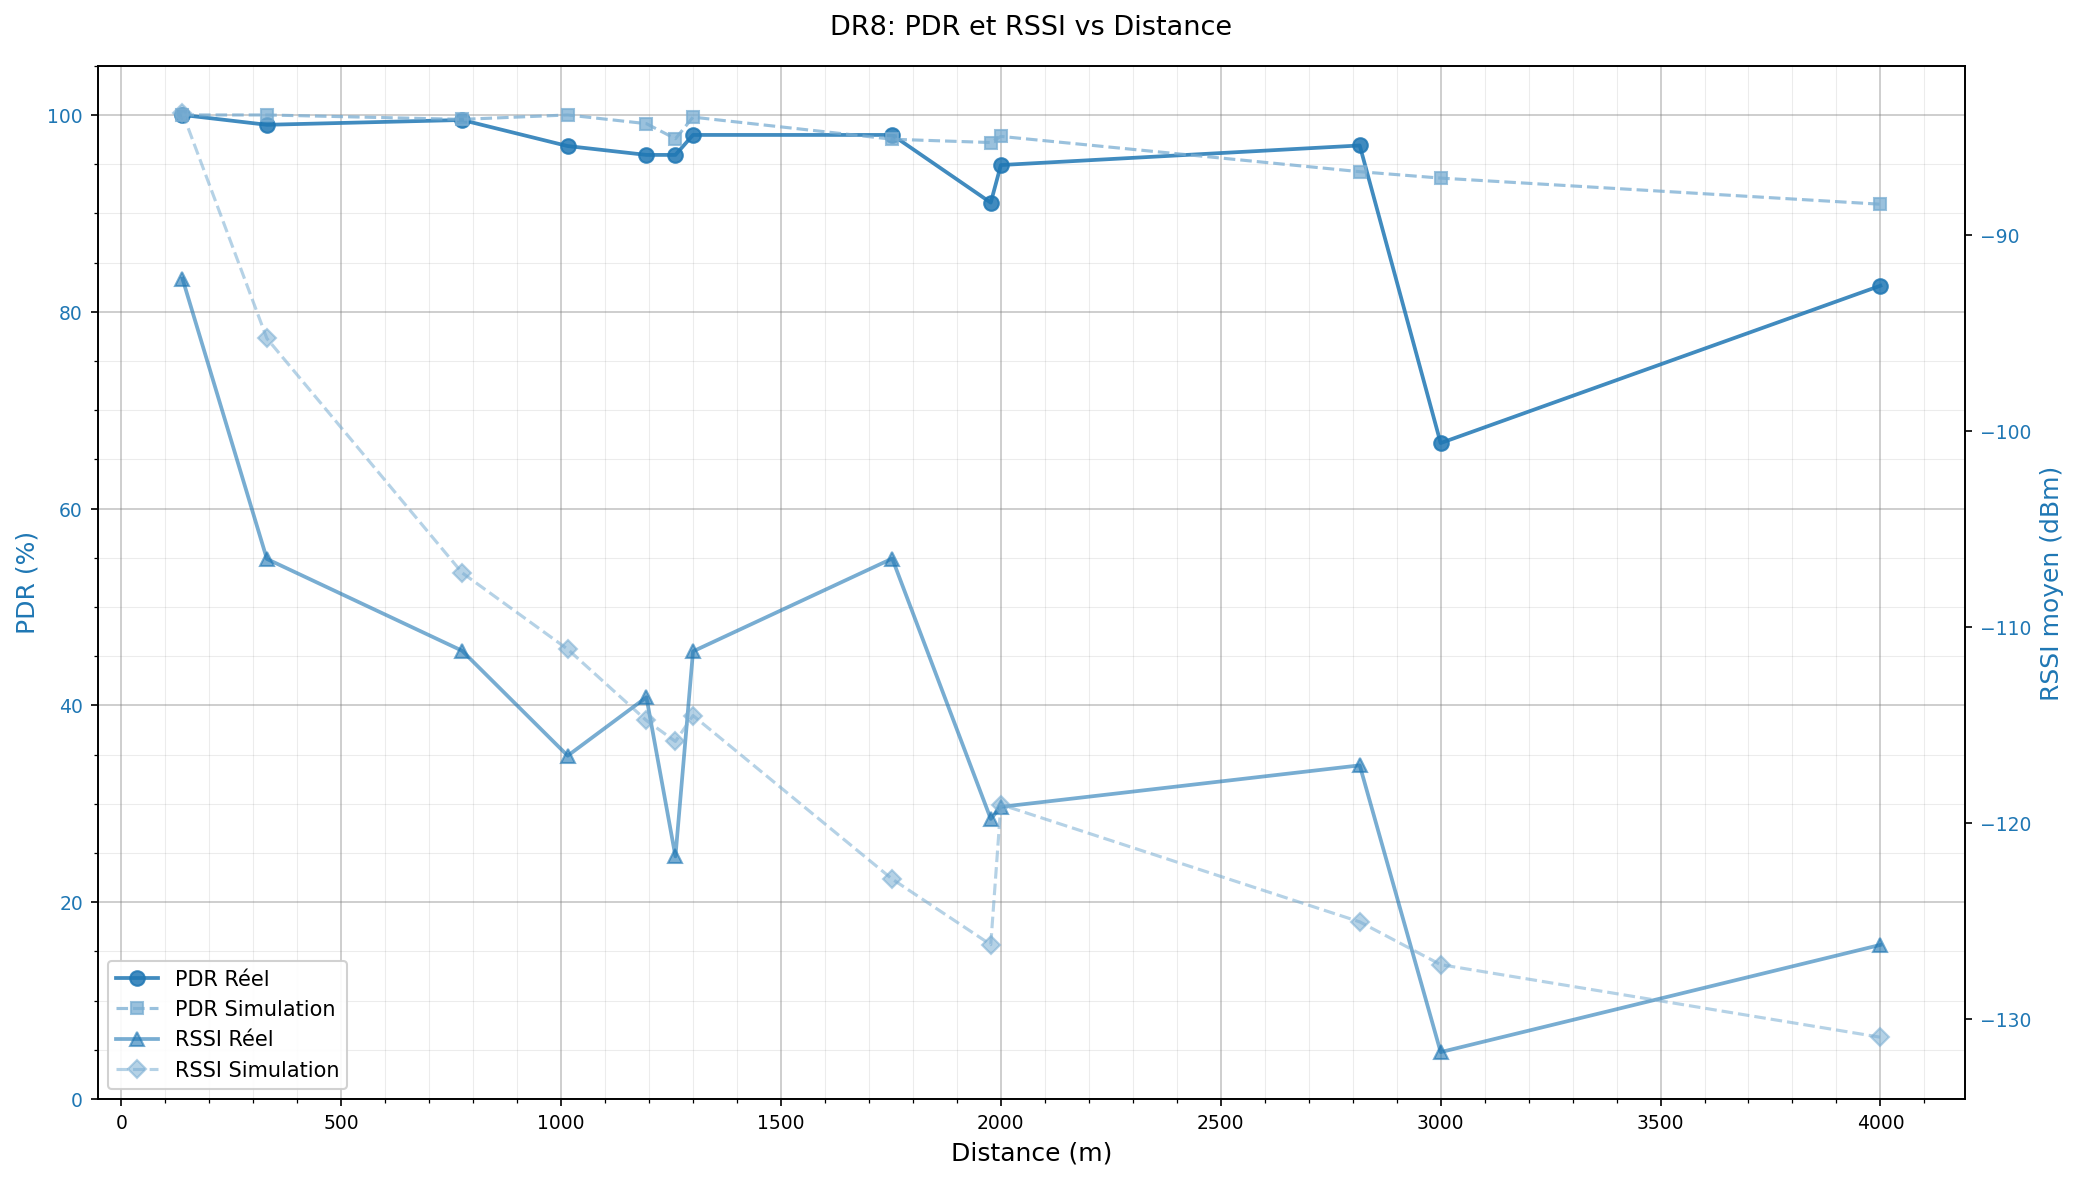
\includegraphics[width=0.8\textwidth]{images/validation/sim/dr8_pdr_rssi_vs_distance.png}
	\caption{Validation du modèle pour DR8 (CR=1/3, BW=137 kHz)}
	\label{fig:dr8_validation}
\end{figure}

Pour le DR8, les résultats montrent une bonne adéquation du modèle de RSSI, avec une erreur moyenne de 7,21 dB sur l'ensemble des distances. Le PDR simulée suit fidèlement la tendance réelle, avec une erreur quadratique moyenne de 10 \%.

\begin{figure}[H]
	\centering
	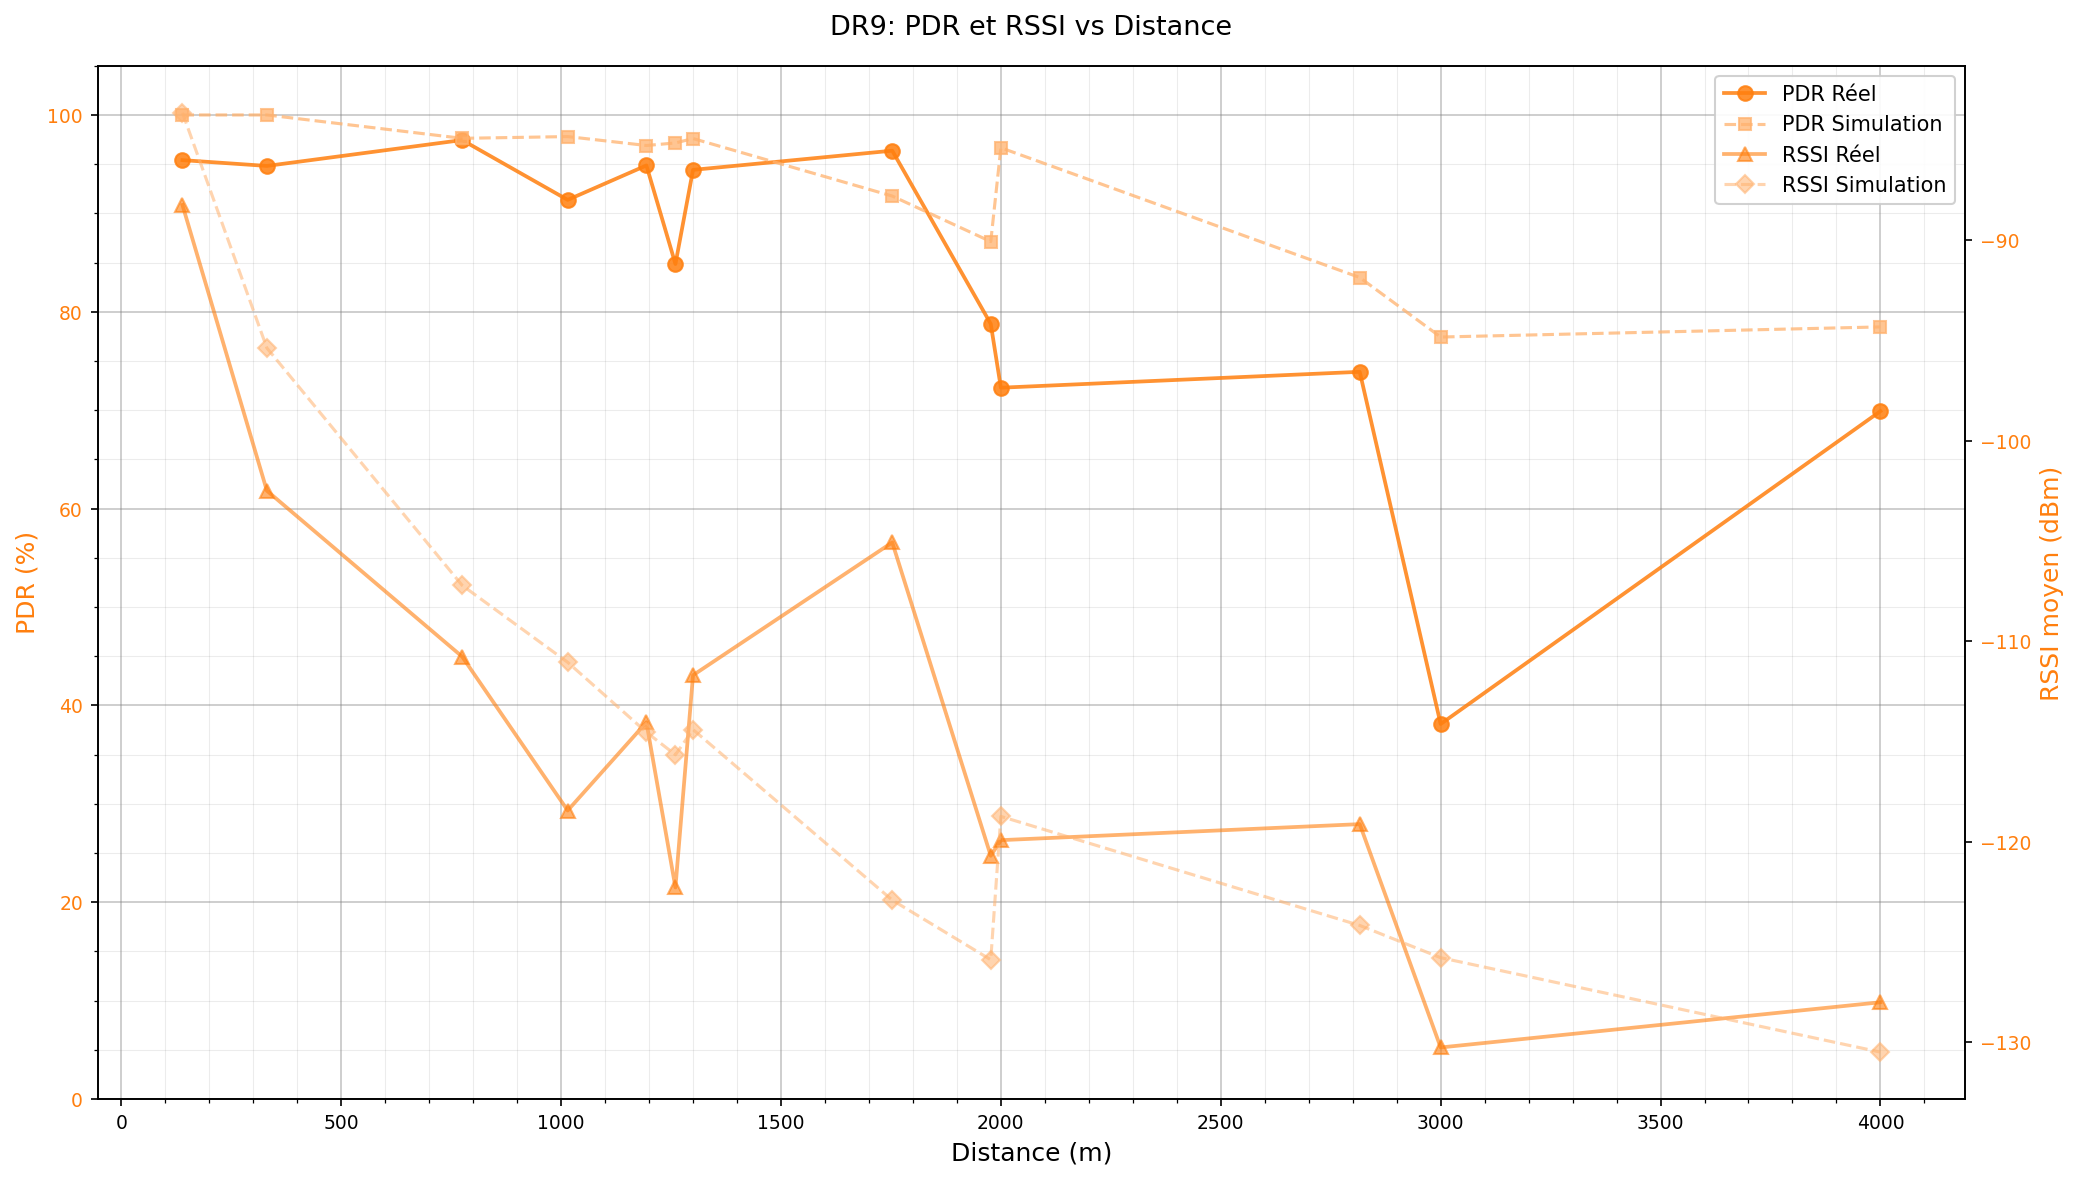
\includegraphics[width=0.8\textwidth]{images/validation/sim/dr9_pdr_rssi_vs_distance.png}
	\caption{Validation du modèle pour DR9 (CR=2/3, BW=137 kHz)}
	\label{fig:dr9_validation}
\end{figure}

Le DR9 montre une sensibilité accrue aux conditions de canal, ce qui se traduit par une décroissance plus rapide du PDR avec la distance. Le simulateur capture correctement cette tendance mais avec une erreur quadratique moyenne du PDR plus élevée de 21,40 \% et du RSSI de 6,84 dB.

\begin{figure}[H]
	\centering
	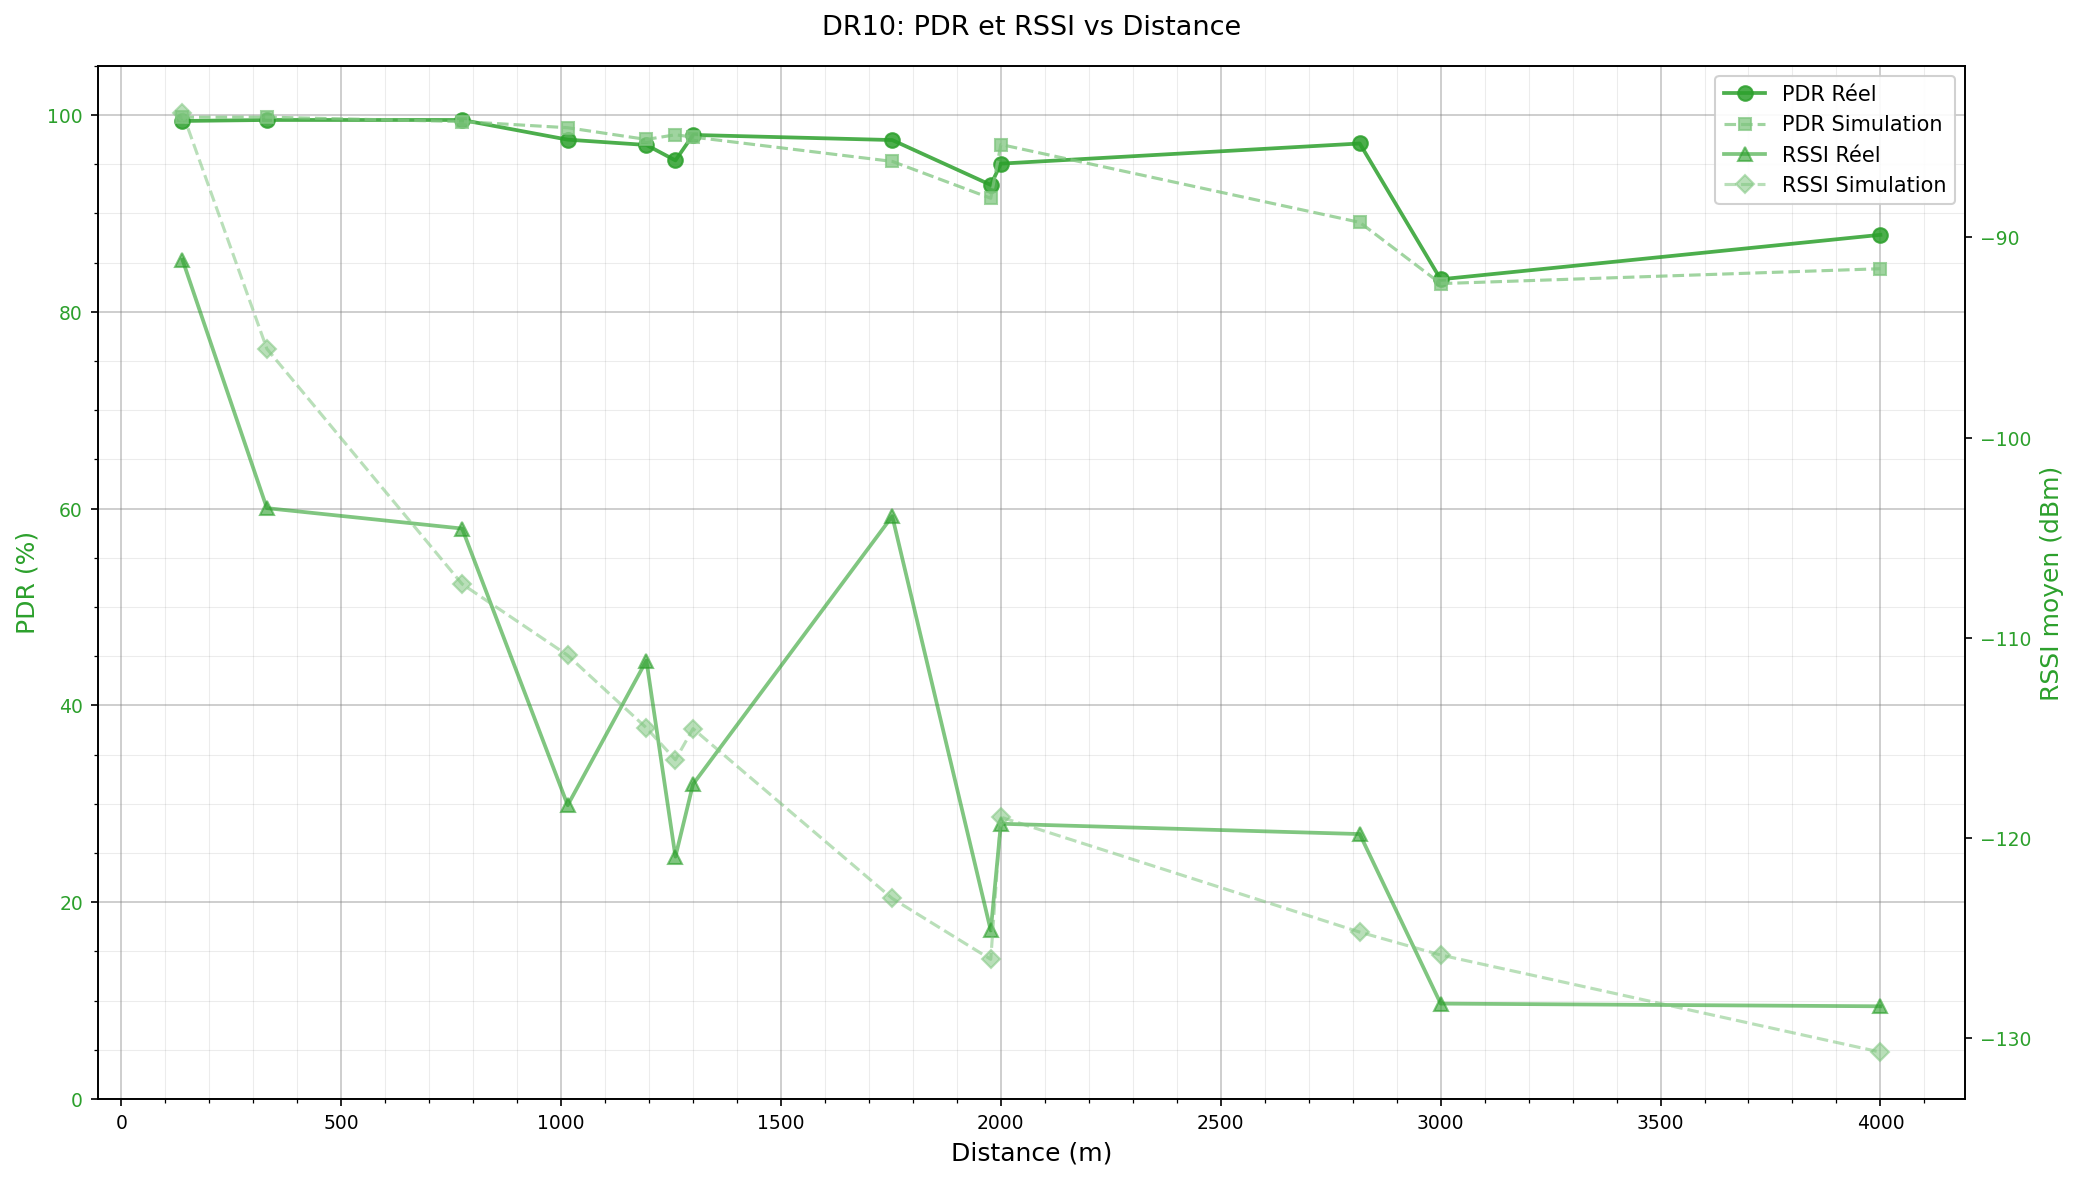
\includegraphics[width=0.8\textwidth]{images/validation/sim/dr10_pdr_rssi_vs_distance.png}
	\caption{Validation du modèle pour DR10 (CR=1/3, BW=336 kHz)}
	\label{fig:dr10_validation}
\end{figure}

Pour les DR à large bande, la validation est tout aussi concluante. Le DR10 maintient une PDR élevée (\(>90\%\)) jusqu'à 2000 m, et la simulation reproduit cette performance avec une grande fidélité. L'erreur quadratique moyenne pour le PDR est de 5,11 \% et pour RSSI 5,92 dB, la meilleure corrélation obtenue.

\begin{figure}[H]
	\centering
	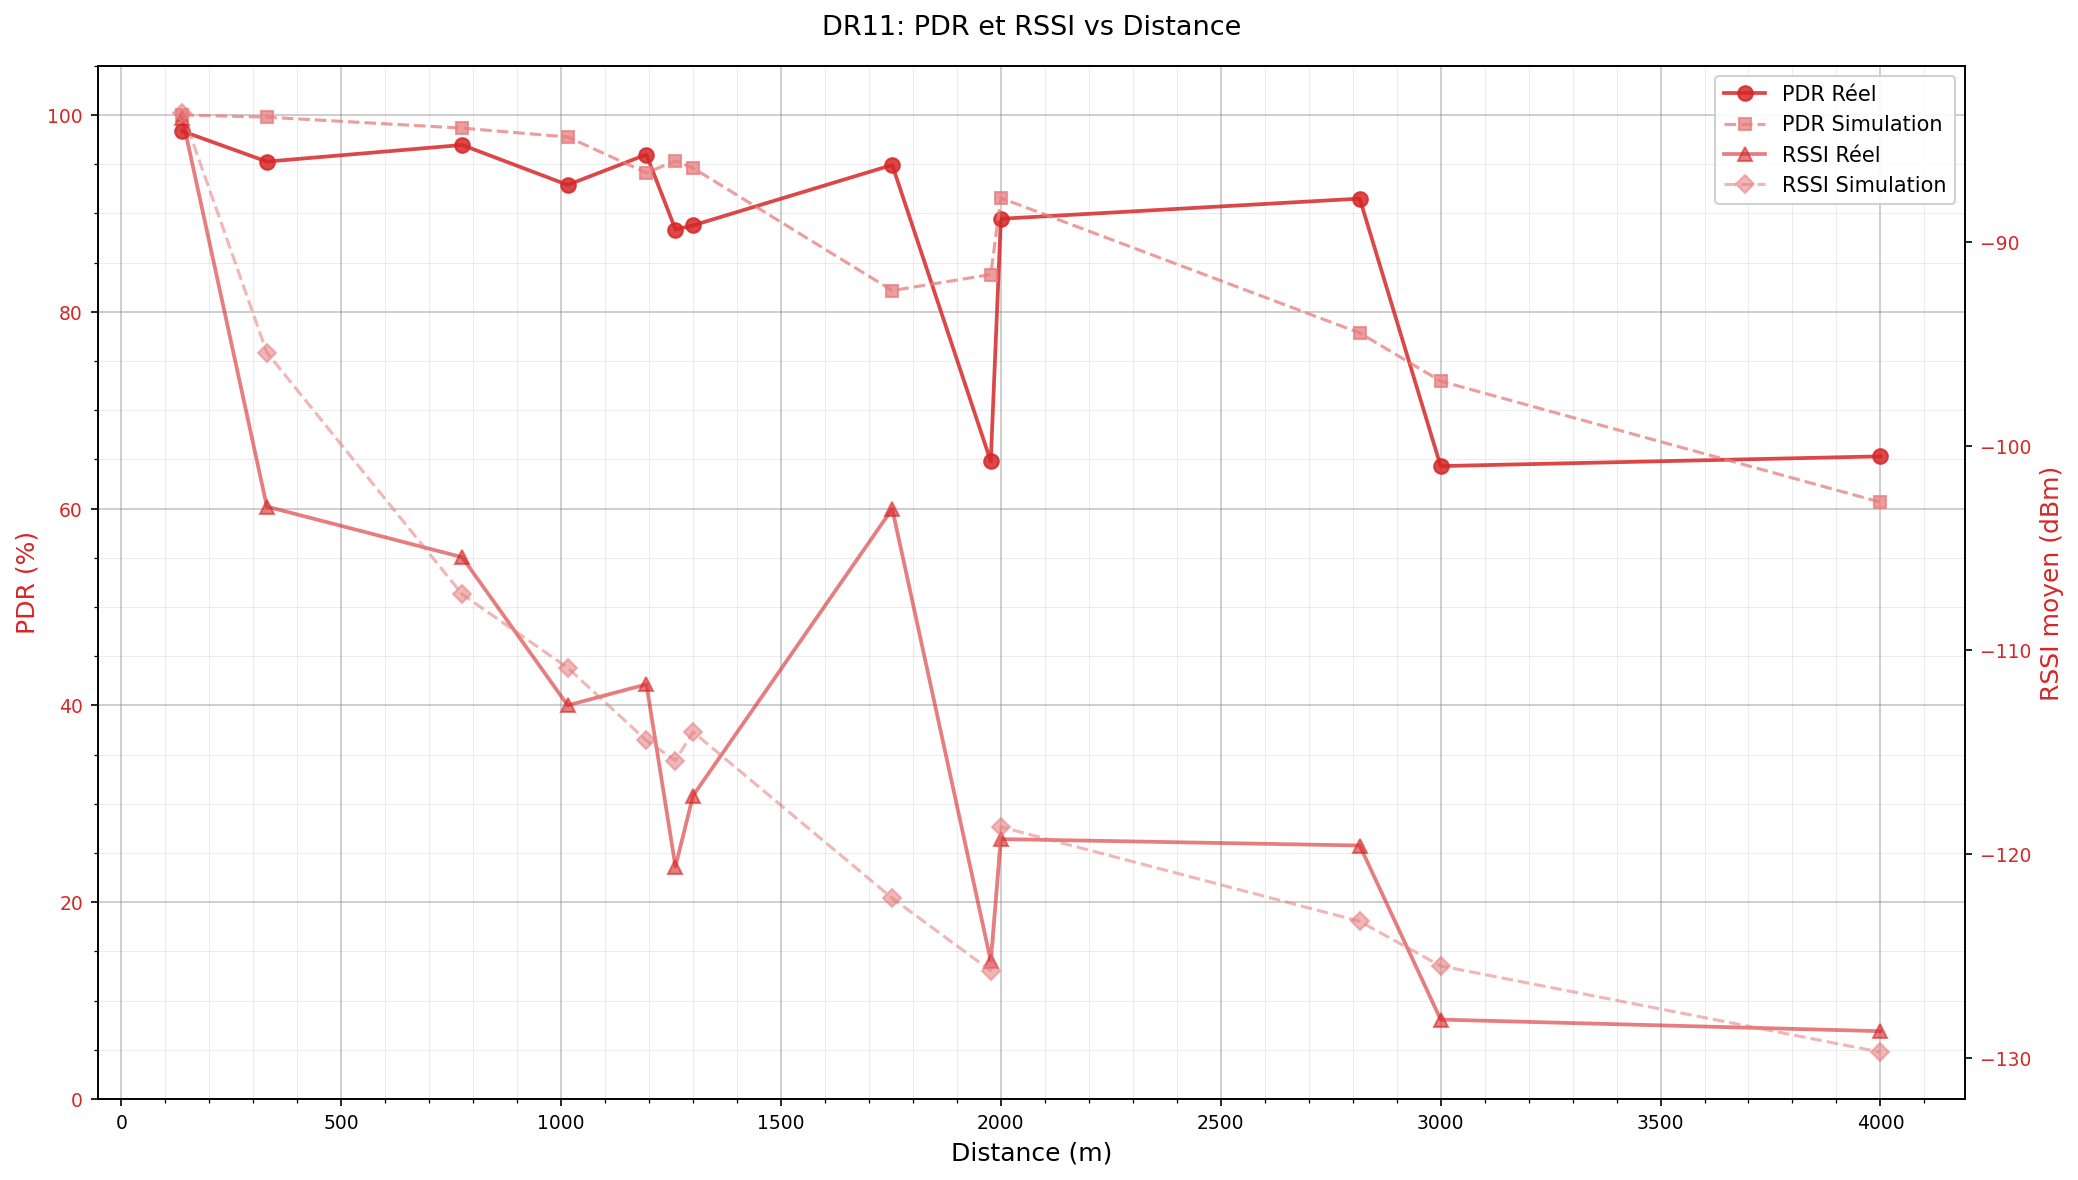
\includegraphics[width=0.8\textwidth]{images/validation/sim/dr11_pdr_rssi_vs_distance.png}
	\caption{Validation du modèle pour DR11 (CR=2/3, BW=336 kHz)}
	\label{fig:dr11_validation}
\end{figure}

Pour le DR11, on constate que le PDR chuter rapidement à partir de 1500 m. La simulation reproduit cette chute avec une erreur quadratique moyenne du PDR de 11,16 \% et pour le RSSI de 6,28 dB.

\newpage
\subsubsection{Analyse globale et quantification des erreurs}

La figure \ref{fig:pdr_global_validation} synthétise les performances de PDR pour l'ensemble des DR.

\begin{figure}[H]
	\centering
	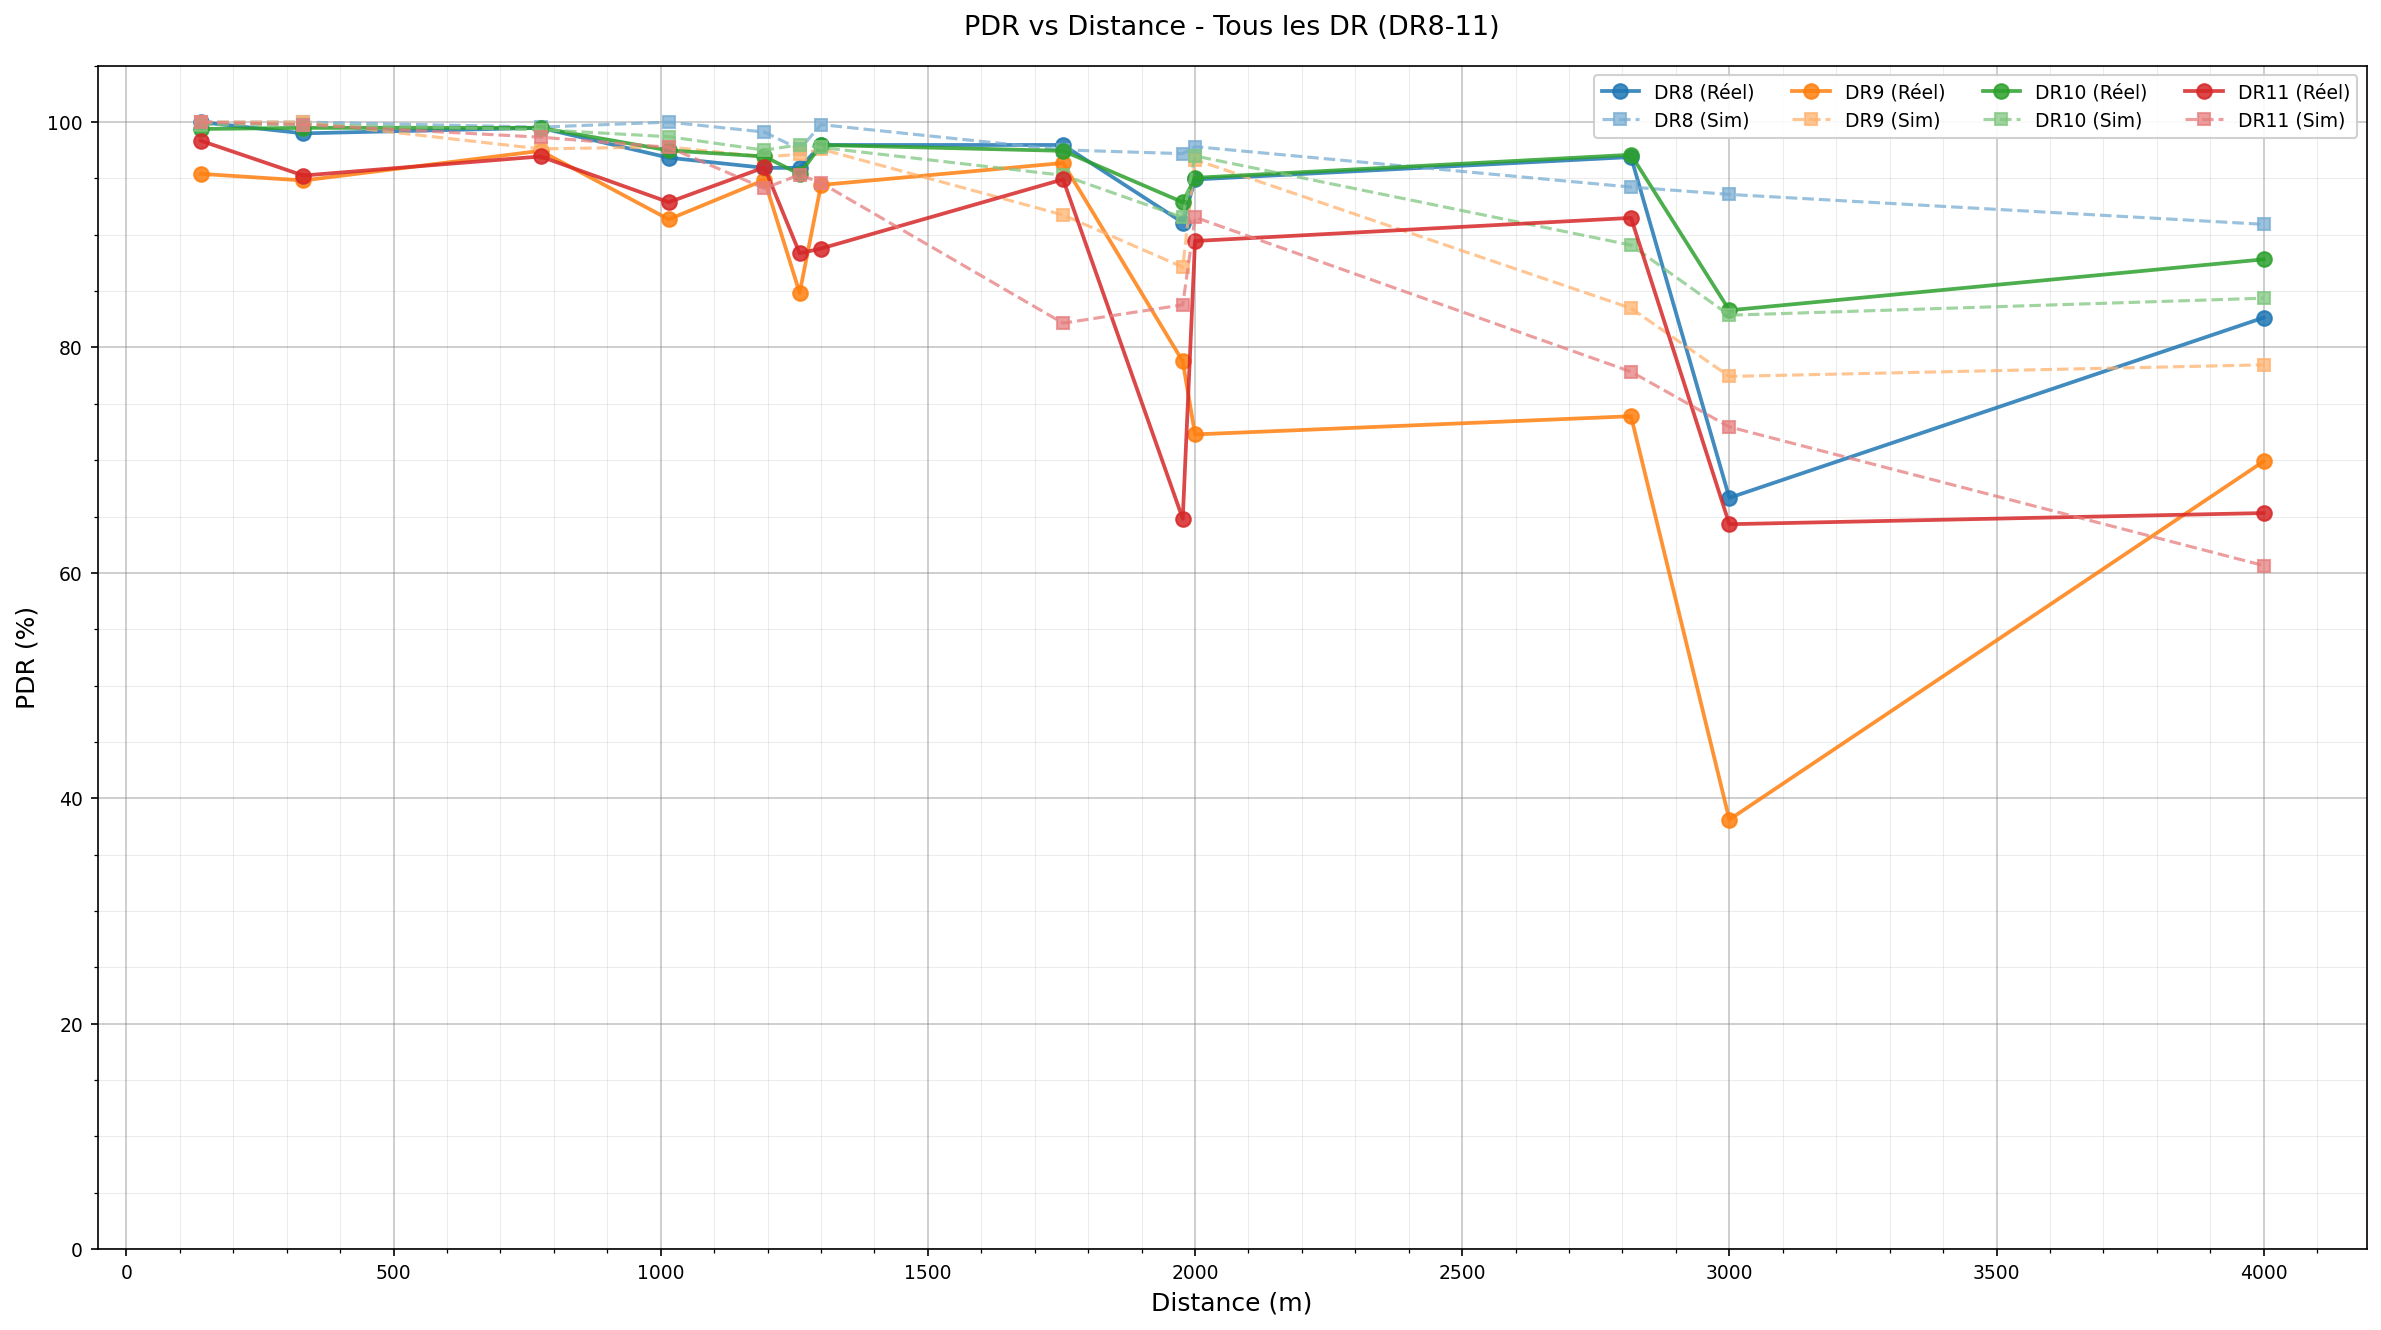
\includegraphics[width=0.9\textwidth]{images/validation/sim/all_dr_pdr_vs_distance.png}
	\caption{Comparaison globale du PDR : simulation et données mesurées}
	\label{fig:pdr_global_validation}
\end{figure}

Les résultats montrent une excellente corrélation globale. Le simulateur parvient à reproduire fidèlement :
\begin{itemize}
	\item La hiérarchie des performances entre les DR
	\item La forme caractéristique des courbes de PDR
\end{itemize}

La figure \ref{fig:rssi_global_validation} montre la comparaison pour le RSSI entre la simulation et les données mesurées.

\begin{figure}[H]
	\centering
	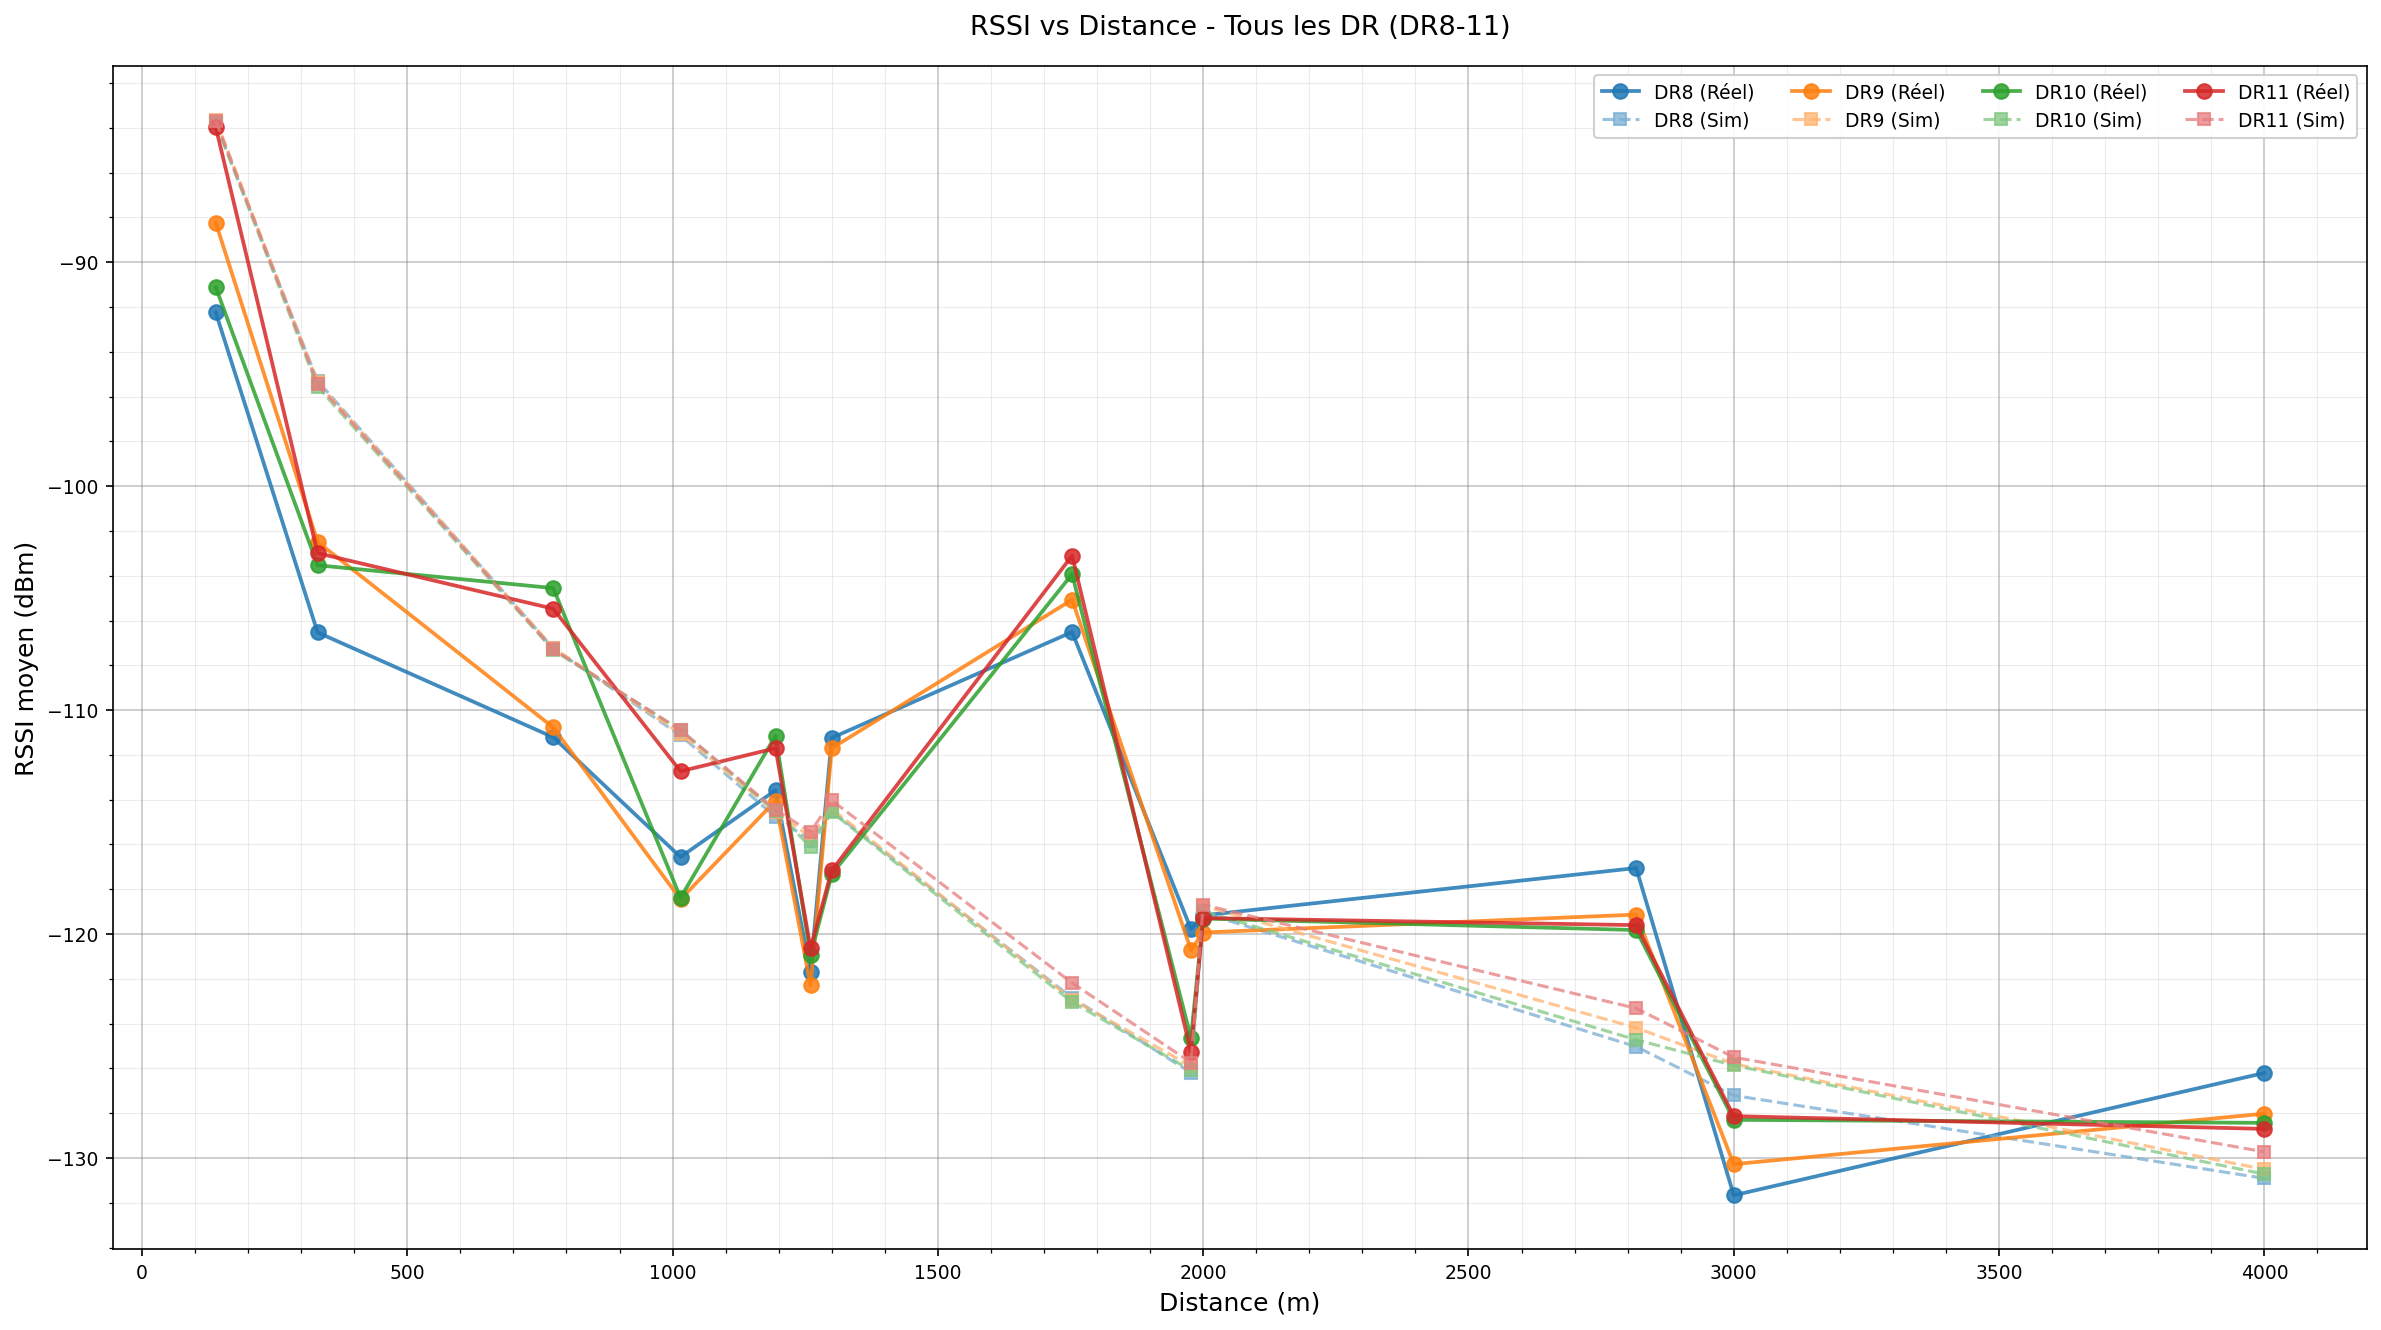
\includegraphics[width=0.9\textwidth]{images/validation/sim/all_dr_rssi_vs_distance.png}
	\caption{Comparaison globale du RSSI moyen}
	\label{fig:rssi_global_validation}
\end{figure}

L'adéquation du modèle de propagation est ici correcte. La simulation prédit le RSSI moyen avec une erreur moyenne de 6,56 dB pour l'ensemble des points de mesure, validant :
\begin{itemize}
	\item Le choix du modèle log-distance avec un exposant \(n=3,3\)
	\item La calibration de la perte de référence à 125 dB à 1 km
	\item Le modèle d'ombrage (\textit{shadowing}) déterministe basé sur la position\\
\end{itemize}

Pour la quantification rigoureuse  de la performance de notre simulateur, nous avons calculé l'erreur quadratique moyenne (RMSE) pour le PDR et le RSSI à l'aide de ces formules :

\begin{equation}
	\text{RMSE}_{\text{PDR}} \; [\%] = \sqrt{\frac{1}{N} \sum_{i=1}^{N} \left( \text{PDR}_{\text{réel},i} - \text{PDR}_{\text{sim},i} \right)^2} \times 100
	\label{eq:rmse_pdr}
\end{equation}

\begin{equation}
	\text{RMSE}_{\text{RSSI}} \; [\text{dB}] = \sqrt{\frac{1}{N} \sum_{i=1}^{N} \left( \text{RSSI}_{\text{réel},i} - \text{RSSI}_{\text{sim},i} \right)^2}
	\label{eq:rmse_rssi}
\end{equation}

où \(N\) est le nombre de points de mesure, \(\text{PDR}_{\text{réel},i}\) et \(\text{PDR}_{\text{sim},i}\) sont respectivement les PDR réelle et simulée au point \(i\), et \(\text{RSSI}_{\text{réel},i}\) et \(\text{RSSI}_{\text{sim},i}\) les RSSI correspondants.

Le tableau suivant fait une synthèse de ces erreurs pour chaque DR.

\begin{table}[H]
	\centering
	\caption{Erreurs quadratiques moyennes (RMSE) entre la simulation et les données réelles}
	\label{tab:validation_errors}
	\begin{tabular}{|c|c|c|}
		\hline
		\textbf{DR} & \textbf{RMSE PDR (\%)} & \textbf{RMSE RSSI (dB)} \\
		\hline
		DR8  & 10,69 & 7,21 \\
		DR9  & 21,40 & 6,84 \\
		DR10 & 5,11  & 5,92 \\
		DR11 & 11,38 & 6,28 \\
		\hline
		\textbf{Moyenne} & \textbf{12,14} & \textbf{6,56} \\
		\hline
	\end{tabular}
\end{table}

Après validation de ce simulateur, nous passons maintenant à l'évaluation de notre solution à l'aide de ce dernier.

\section{Méthodologie d'évaluation}
\label{sec:methodo-eval}
Cette sous-section détaille la méthodologie adoptée pour évaluer les performances de l’agent DDQN. Elle présente d’abord le protocole de simulation utilisé pour reproduire des scénarios réalistes, puis définit les métriques de performance retenues pour analyser la fiabilité, l’efficacité énergétique et l’adaptativité des transmissions

\subsection{Protocole}
\label{subsec:protocole-eval}

Pour garantir la reproductibilité et la pertinence de nos résultats, nous avons mis en place un protocole d'évaluation rigoureux :

\begin{enumerate}
	\item \textbf{Points de comparaison} : Nous utilisons les 13 distances du fichier de validation \cite{sanchez_vital_2025_data}, couvrant une plage de 139 m à 4000 m.
	\item \textbf{Configurations testées} :
	\begin{itemize}
		\item \textbf{Simulation standard} : Pour chaque distance et chaque DR, nous exécutons une simulation de 30 minutes avec 10 nœuds, paramétrée avec les caractéristiques physiques du DR et une puissance d'émission fixe de 14 dBm.
		\item \textbf{Simulation avec DDQN} : Pour chaque distance, nous exécutons une simulation où l'agent DDQN sélectionne dynamiquement le DR et la puissance pour chaque transmission.
	\end{itemize}
	\item \textbf{Métriques collectées} : Pour chaque simulation, nous enregistrons le PDR global, la distribution des choix de DR et de puissance, et la consommation énergétique par transmission.
	\item \textbf{Reproductibilité} : Pour chacune de ces simulations, nous avons les mêmes conditions : mêmes positions, même ombrage et même évaluation grâce à une \textit{seed} globale que nous pouvons faire varier.
\end{enumerate}

\subsection{Métriques de performance}
\label{subsec:metriques-eval}

Les performances sont évaluées selon trois axes :

\begin{itemize}
	\item \textbf{La fiabilité} : \(\text{PDR} = \frac{\text{Nombre de paquets reçus avec succès}}{\text{Nombre total de paquets émis}}\)
	\item \textbf{L'efficacité énergétique} : \(E_{\text{tx}} = \text{Énergie consommée par transmission} \ [\text{mJ}]\)
	\item \textbf{L'adaptativité} : Analysée à travers la distribution des choix de DR et de puissance en fonction de la distance.
\end{itemize}

\section{Résultats et analyse comparative}
\label{sec:resultats-analyse}
Cette section présente les résultats obtenus lors des simulations et analyse de manière comparative les performances entre la configuration statique (standard) et l’agent DDQN. Les évaluations sont effectuées globalement, puis détaillées selon les distances, le PDR, le débit, la puissance d’émission et la consommation énergétique.

\subsection{Analyse globale des performances}

La figure \ref{fig:pdr-comparison} présente une comparaison globale du PDR entre la simulation standard et la simulation avec DDQN.

\begin{figure}[H]
	\centering
	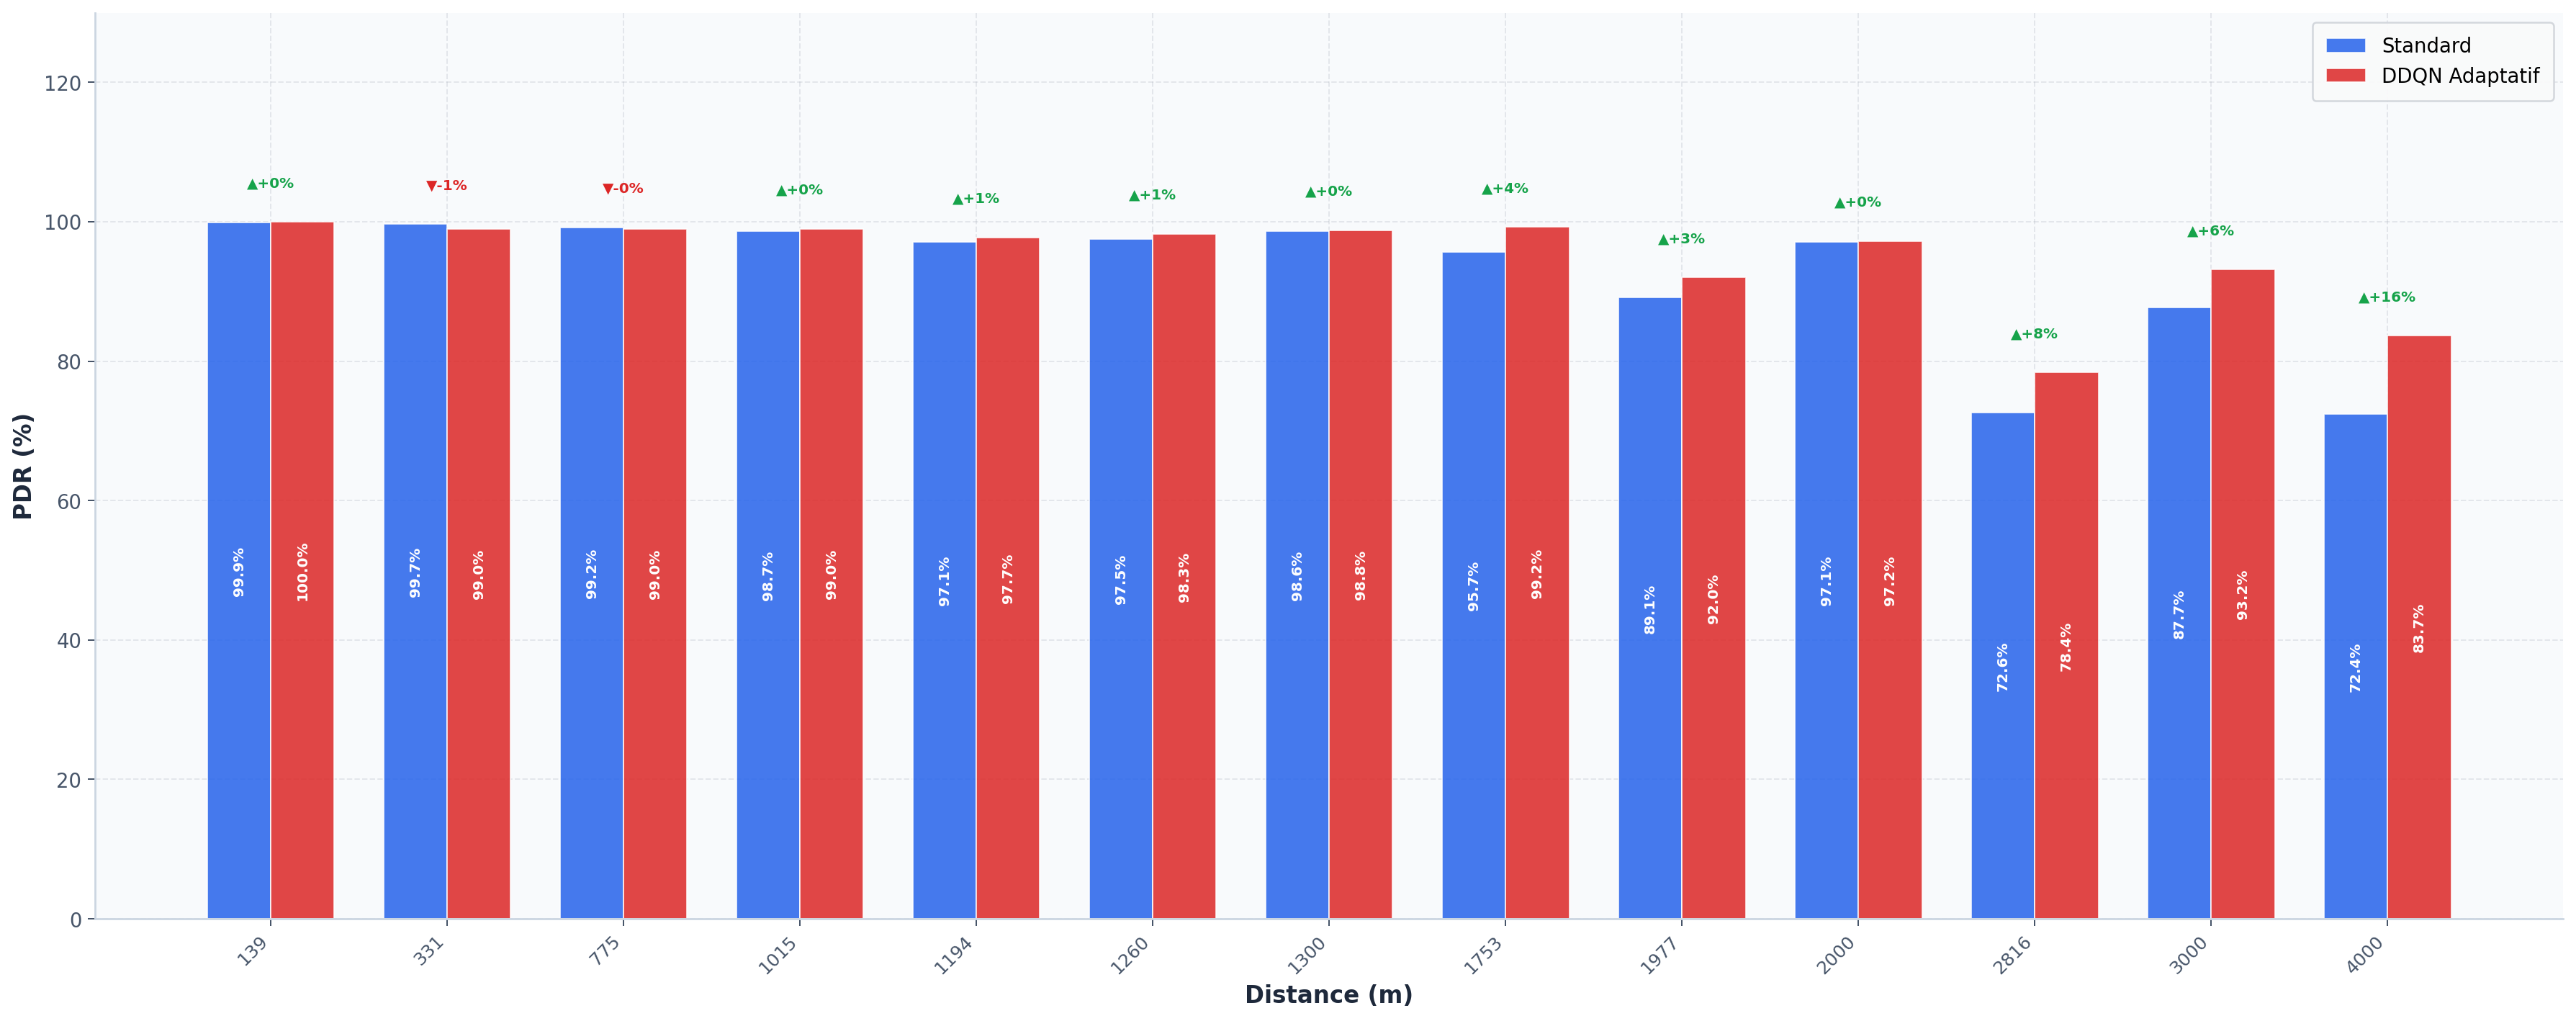
\includegraphics[width=1\textwidth]{images/validation/ddqn/pdr_by_distance.png}
	\caption{Comparaison du PDR entre simulation standard et agent DDQN}
	\label{fig:pdr-comparison}
\end{figure}

L'agent DDQN maintient un PDR systématiquement supérieur, particulièrement visible aux distances moyennes et longues : à 1753 m (99,2\% contre 95,7\%), à 2816 m (78,4\% contre 72,6\%), et à 4000 m (83,7\% contre 72,4\%, soit un gain absolu de 11,3 points et une amélioration relative de 15,6\%).

\subsection{Analyse de la stratégie d'adaptation du DDQN}

La figure \ref{fig:ddqn-dr-choices} illustre la distribution des choix de DR effectués par l'agent DDQN en fonction de la distance et la figure \ref{fig:ddqn-debit} l'évolution du débit découlant du choix du DR.

\begin{figure}[H]
	\centering
	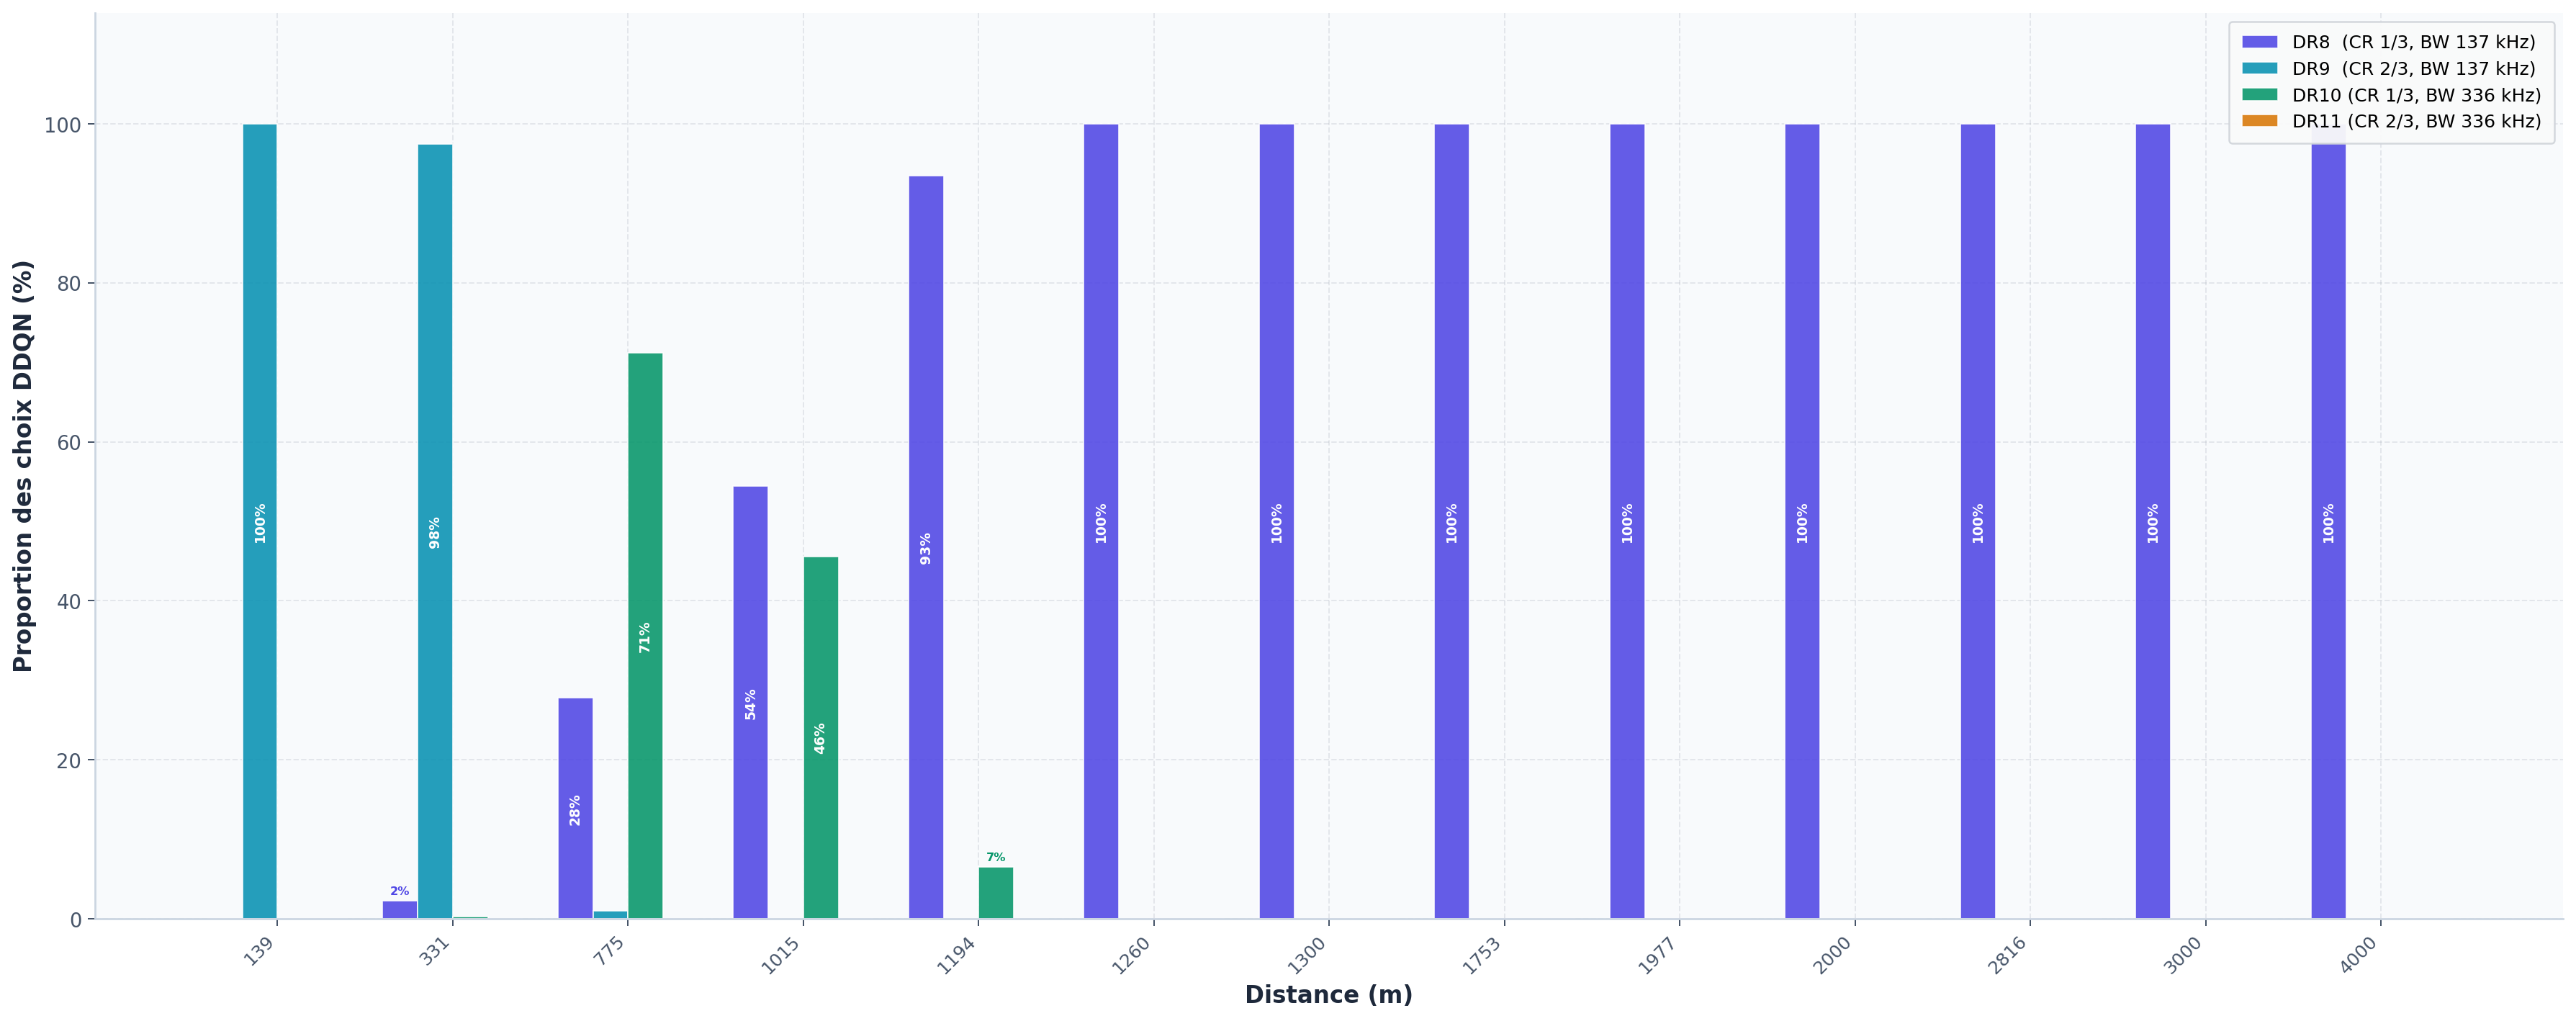
\includegraphics[width=1\textwidth]{images/validation/ddqn/ddqn_dr_choices.png}
	\caption{Distribution des DR choisis par l'agent DDQN en fonction de la distance}
	\label{fig:ddqn-dr-choices}
\end{figure}

\begin{figure}[H]
	\centering
	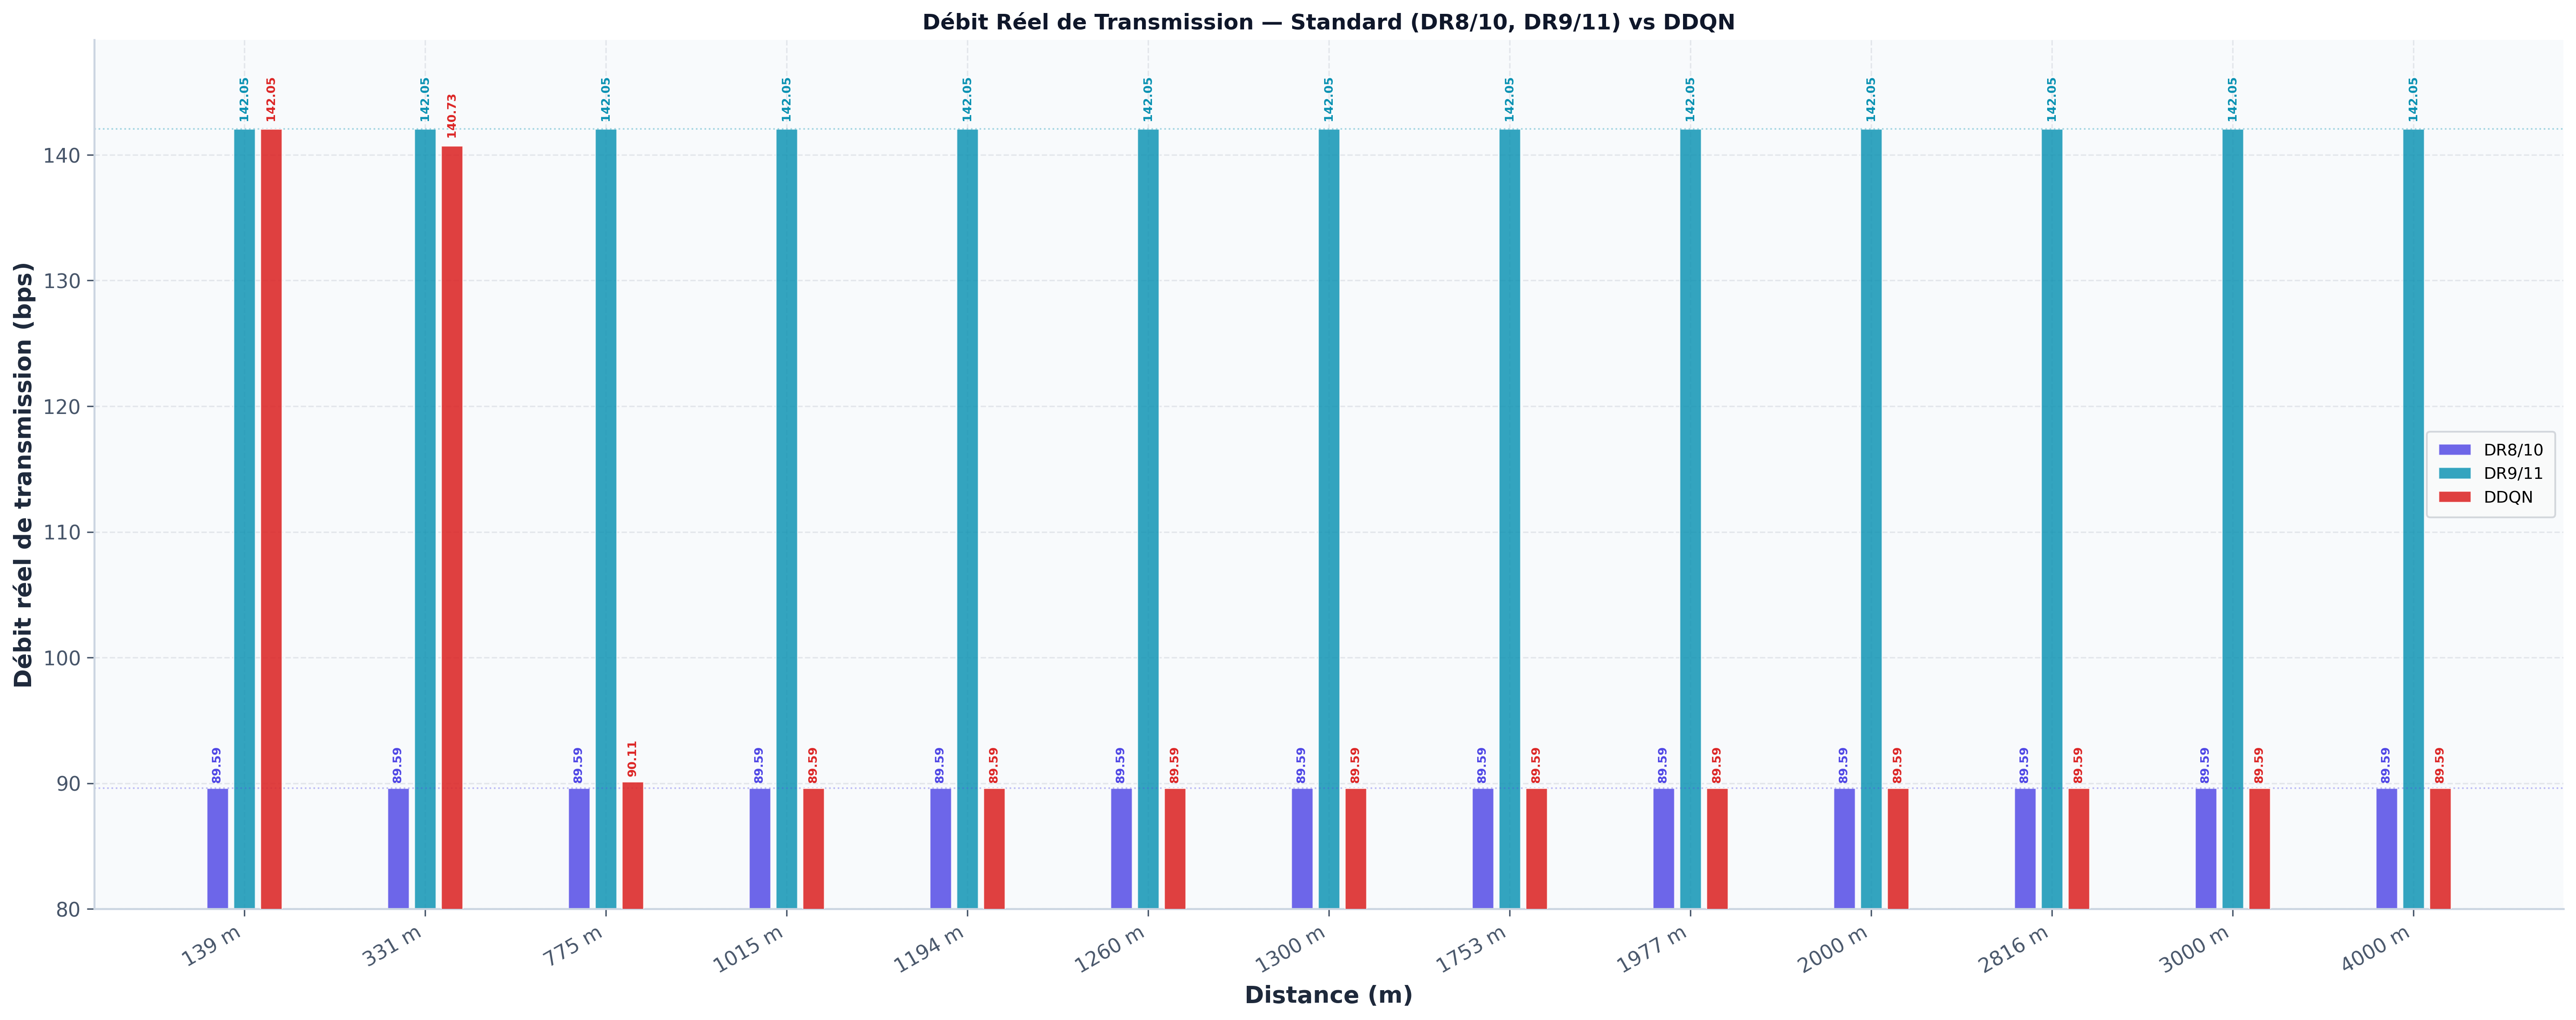
\includegraphics[width=1\textwidth]{images/validation/ddqn/debit_brut.png}
	\caption{Évolution du débit résultant du choix de DR}
	\label{fig:ddqn-debit}
\end{figure}

La politique d'adaptation est claire et progressive :
\begin{itemize}
	\item À courte distance (139 m), le DDQN atteint son \textbf{débit maximal} de 142,05 bps. Cela s'explique par l'utilisation exclusive des DR9/11 (100\%), qui permettent un débit plus élevé.
	
	\item À  331 m, le DDQN reste proche du débit  maximal (140,73 bps), grâce à une utilisation encore majoritaire de DR9/11 (98 \%) et DR8/10 (2 \%).
	
	\item À moyenne distance (775 m), le débit du DDQN chute à 90,11 bps. Cela correspond à une transition vers les DR8/10 (99\%) et DR9/11 (1\%), utilisé pour maintenir la fiabilité des transmissions à plus longue distance.
	
	\item Sur les longues distances (1015–4000 m), le DDQN utilise exclusivement le DR8/10 (100\%), ce qui explique le débit réduit (89,59 bps). Cette stratégie illustre la capacité de l'agent DDQN à adapter dynamiquement le DR en fonction de la distance pour maximiser la fiabilité au détriment d'un débit élevé.
	
	\item En comparaison, la moyenne entre DR8/10 et DR9/11 est de 115,82 bps, mais le DDQN peut dépasser cette moyenne à courte distance grâce à la sélection intelligente du DR le plus performant.
\end{itemize}

Cette stratégie est alignée avec la théorie des communications : utiliser les DR les plus efficaces (haut débit) quand le canal le permet, et basculer vers des configurations robustes quand les conditions se dégradent.

\subsection{Analyse comparative détaillée par DR}

Pour valider la stratégie d'adaptation de l'agent DDQN, nous avons comparé ses performances pour chaque configuration de DR (DR8 à DR11). Les figures \ref{fig:dr8-pdr} à \ref{fig:dr11-rssi} présentent la comparaison des PDR et des RSSI pour chaque DR.

\newpage
\begin{itemize}
	\item \textbf{Analyse pour DR8 (CR 1/3, BW 137 kHz)}
	
	\begin{figure}[H]
		\centering
		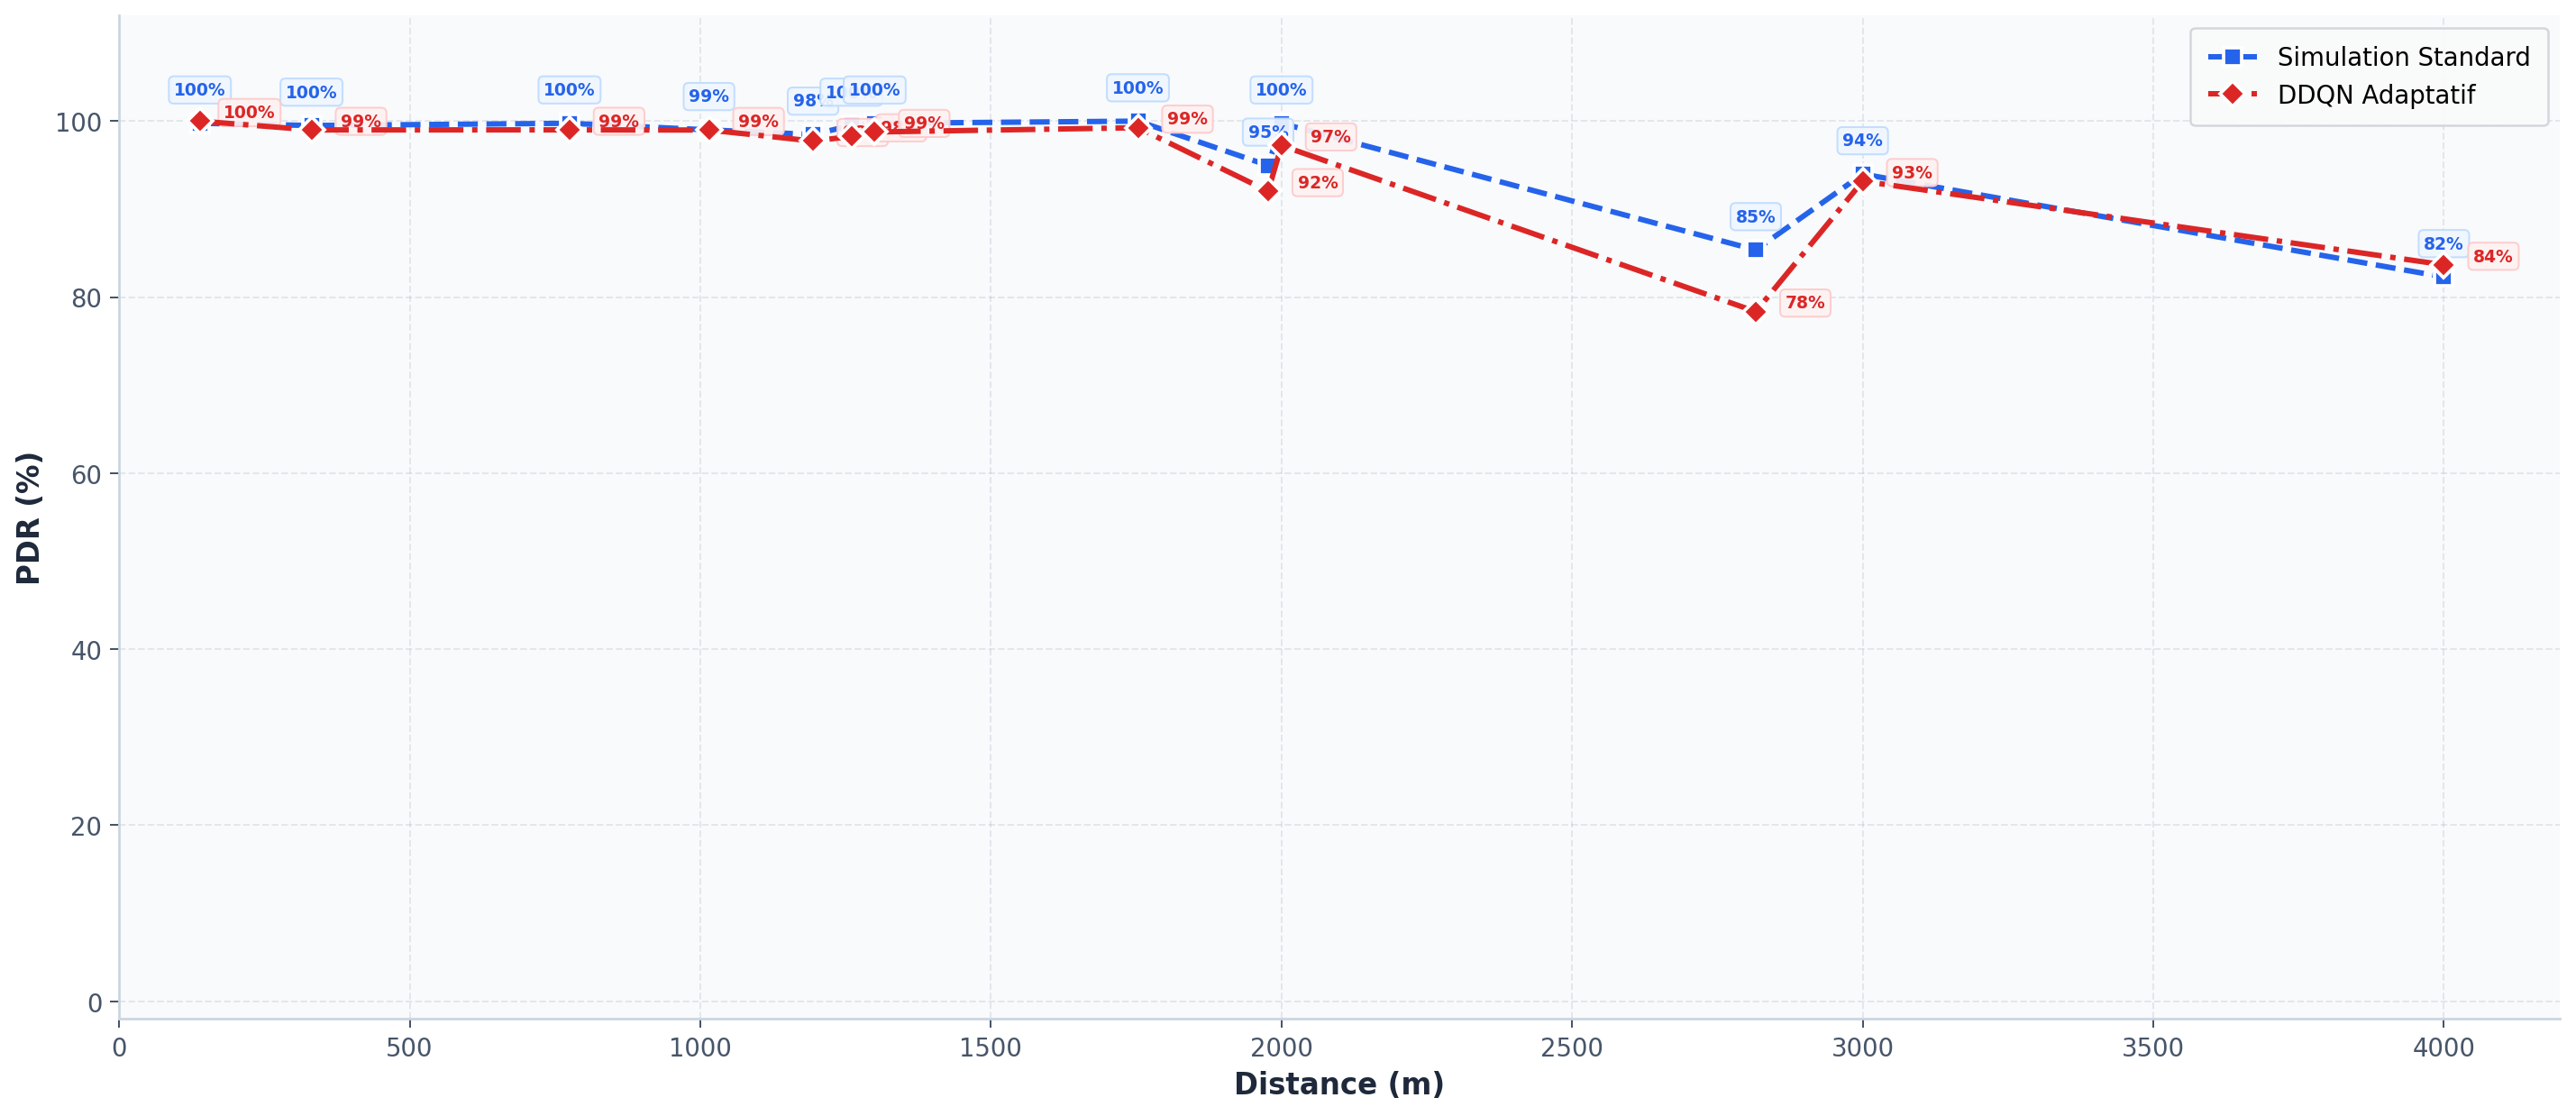
\includegraphics[width=1\textwidth]{images/validation/ddqn/dr/dr8_pdr_courbes.png}
		\caption{Comparaison PDR pour DR8 : Standard vs DDQN}
		\label{fig:dr8-pdr}
	\end{figure}
	
	\begin{figure}[H]
		\centering
		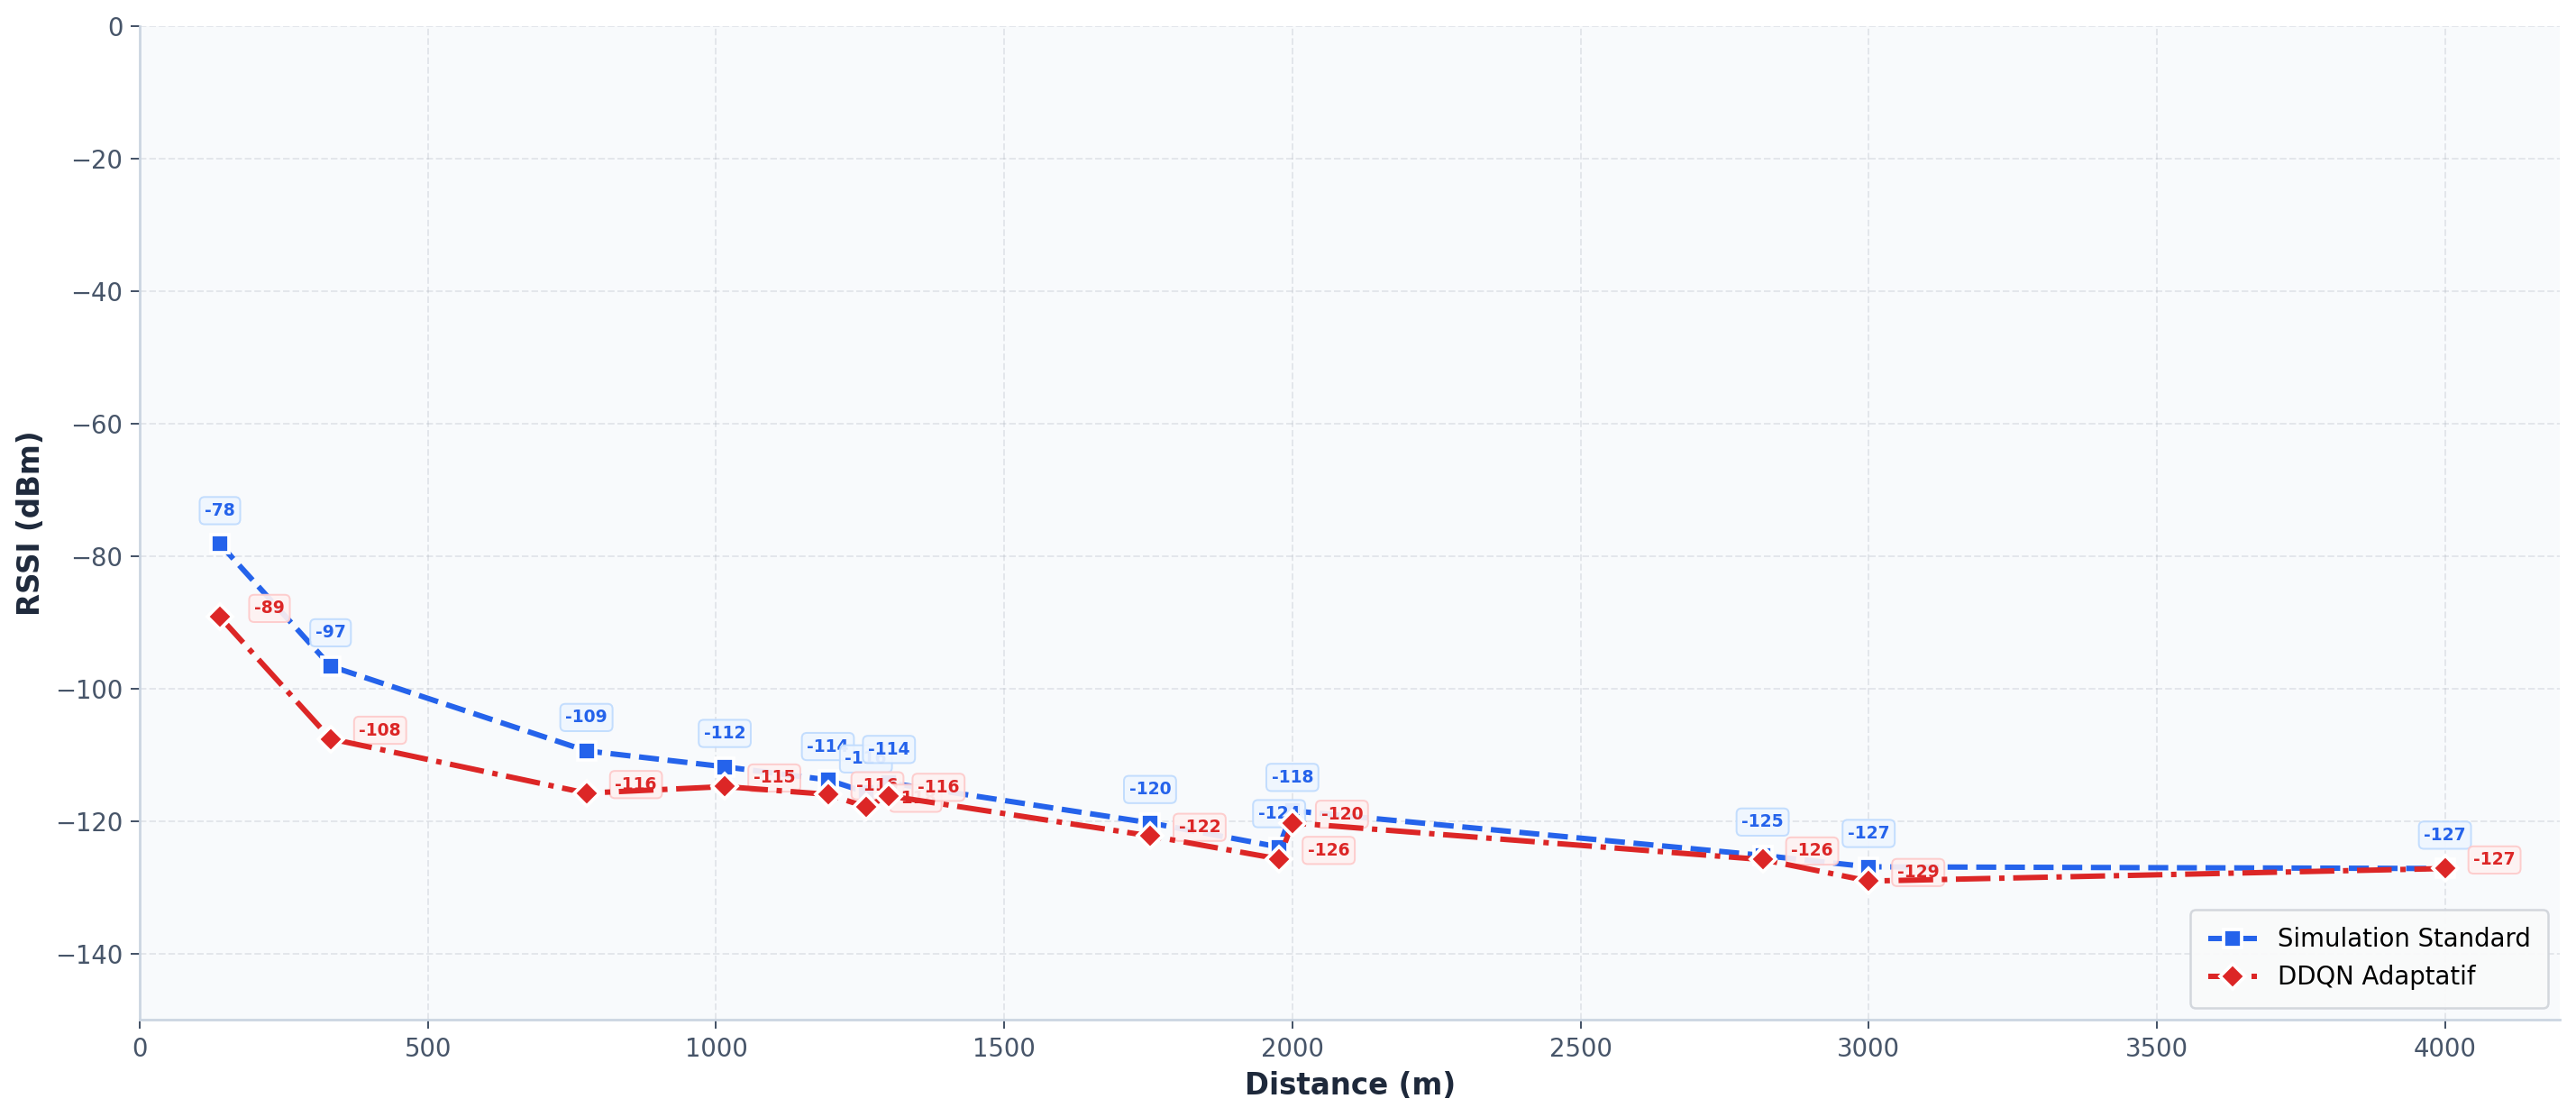
\includegraphics[width=1\textwidth]{images/validation/ddqn/dr/dr8_rssi_courbes.png}
		\caption{Comparaison RSSI pour DR8 : Standard vs DDQN}
		\label{fig:dr8-rssi}
	\end{figure}
	
	Pour le DR8, l'agent DDQN démontre un bon niveau de performance. Grâce à l'utilisation adaptative de différents débits (DR) et niveaux de puissance d'émission, l'agent DDQN parvient à obtenir des résultats comparables à ceux obtenus avec l'utilisation exclusive du DR8 à puissance d'émission maximale de 14 dBm.
	
	\newpage
	\item \textbf{Analyse pour DR9 (CR 2/3, BW 137 kHz)}
	
	\begin{figure}[H]
		\centering
		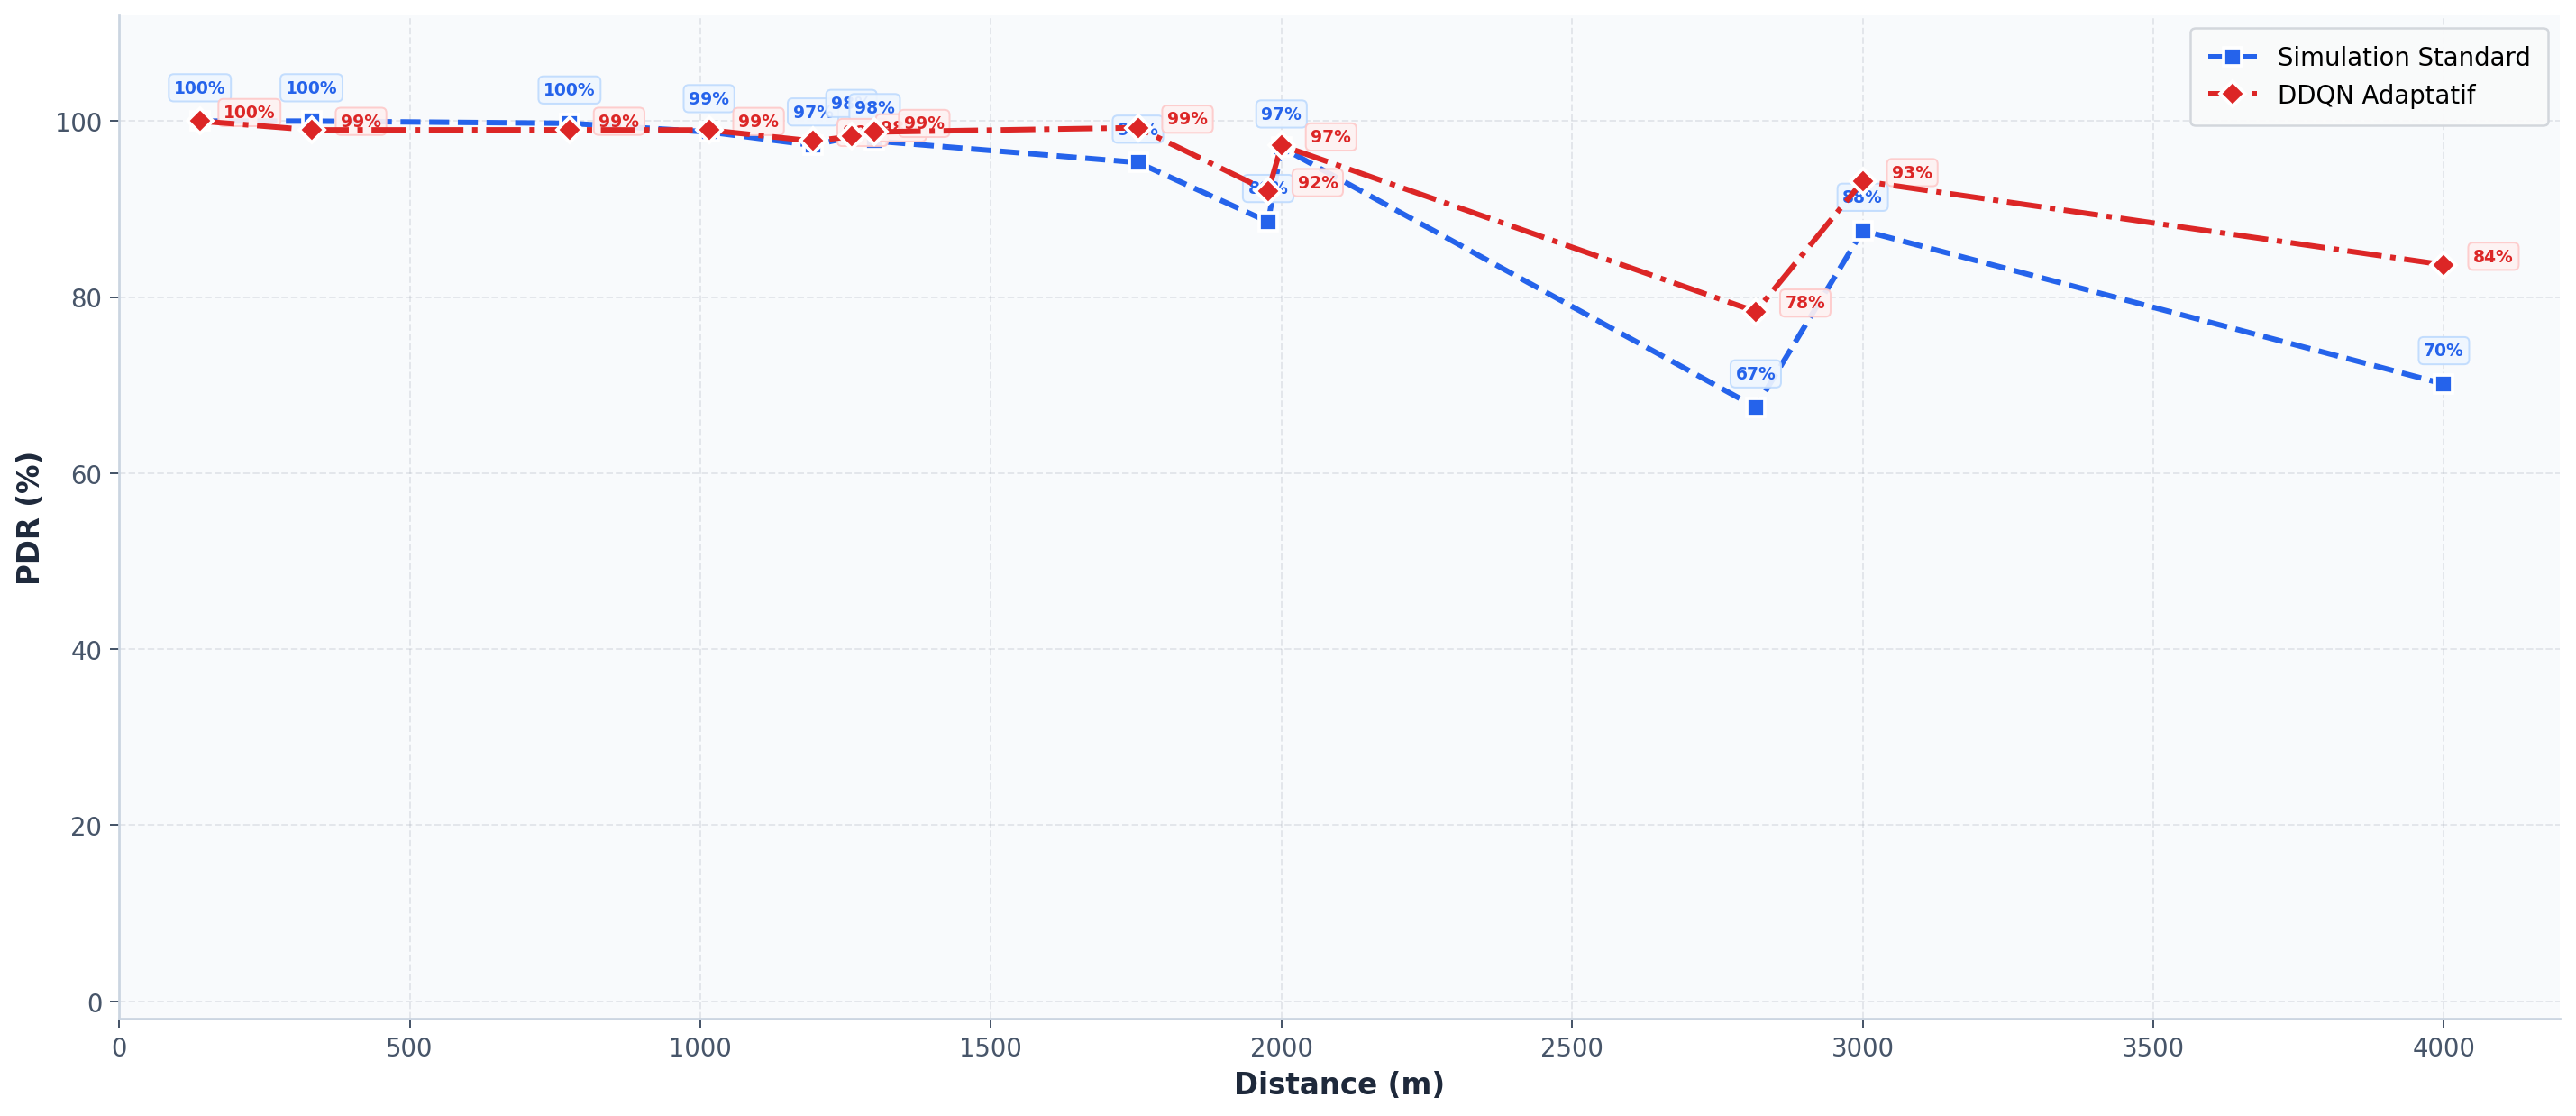
\includegraphics[width=1\textwidth]{images/validation/ddqn/dr/dr9_pdr_courbes.png}
		\caption{Comparaison PDR pour DR9 : Standard vs DDQN}
		\label{fig:dr9-pdr}
	\end{figure}
	
	\begin{figure}[H]
		\centering
		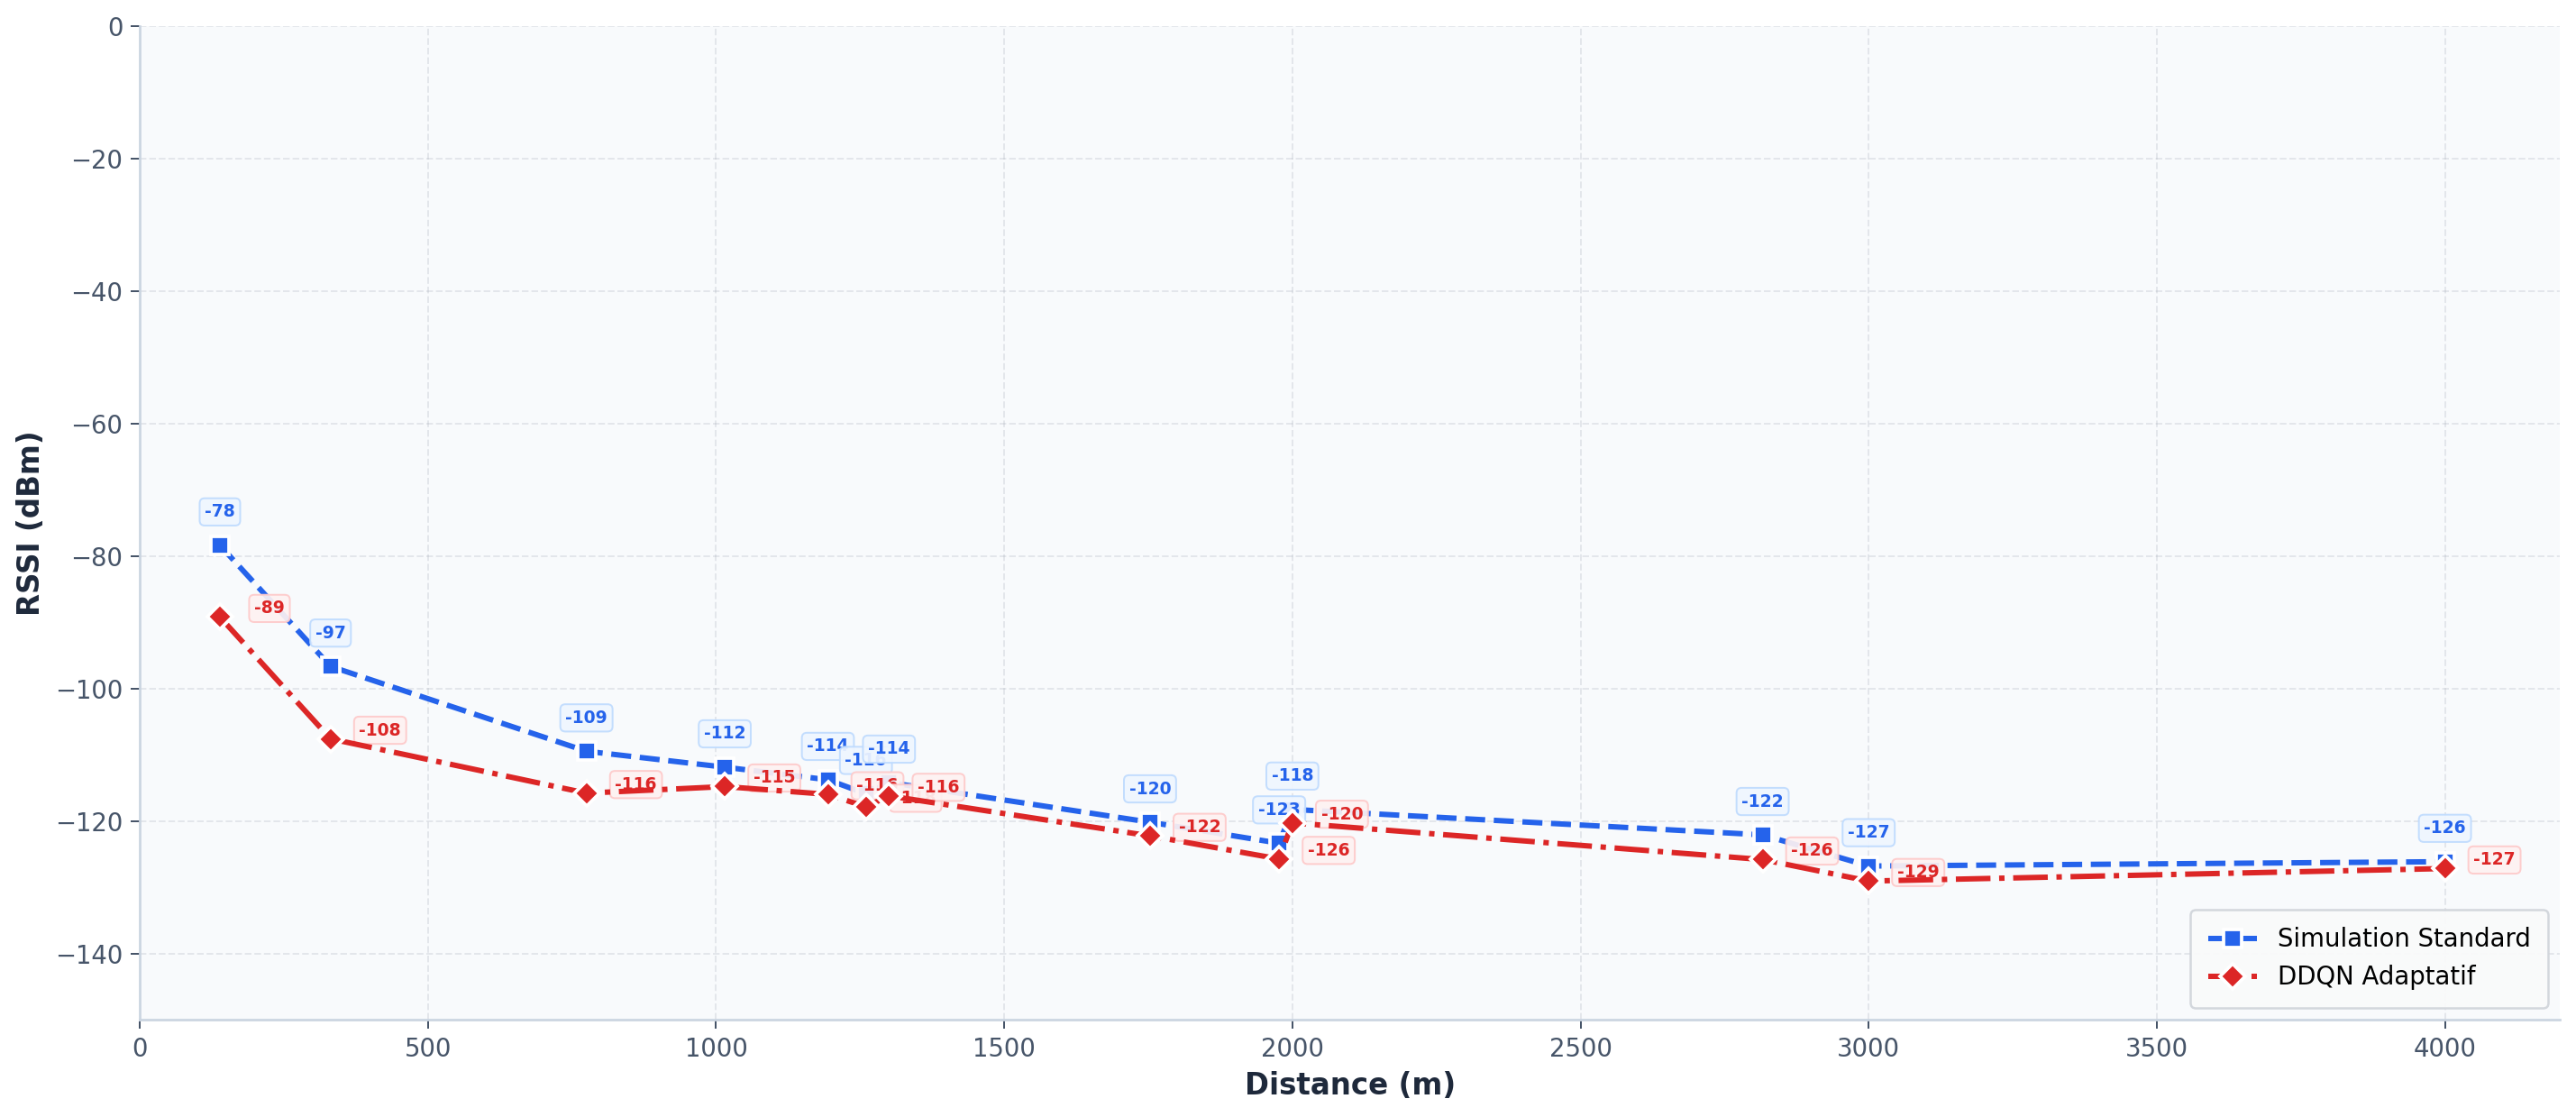
\includegraphics[width=1\textwidth]{images/validation/ddqn/dr/dr9_rssi_courbes.png}
		\caption{Comparaison RSSI pour DR9 : Standard vs DDQN}
		\label{fig:dr9-rssi}
	\end{figure}
	
	Pour le DR9, l'agent DDQN montre une nette supériorité, en particulier aux moyennes et longues distances. Notamment à 4000 m, il atteint un PDR de 84\%, contre 70\% pour la simulation standard, soit un gain absolu de 14 points et une amélioration relative d'environ 20\%.
	
	\newpage
	\item \textbf{Analyse pour DR10 (CR 1/3, BW 336 kHz)}
	
	\begin{figure}[H]
		\centering
		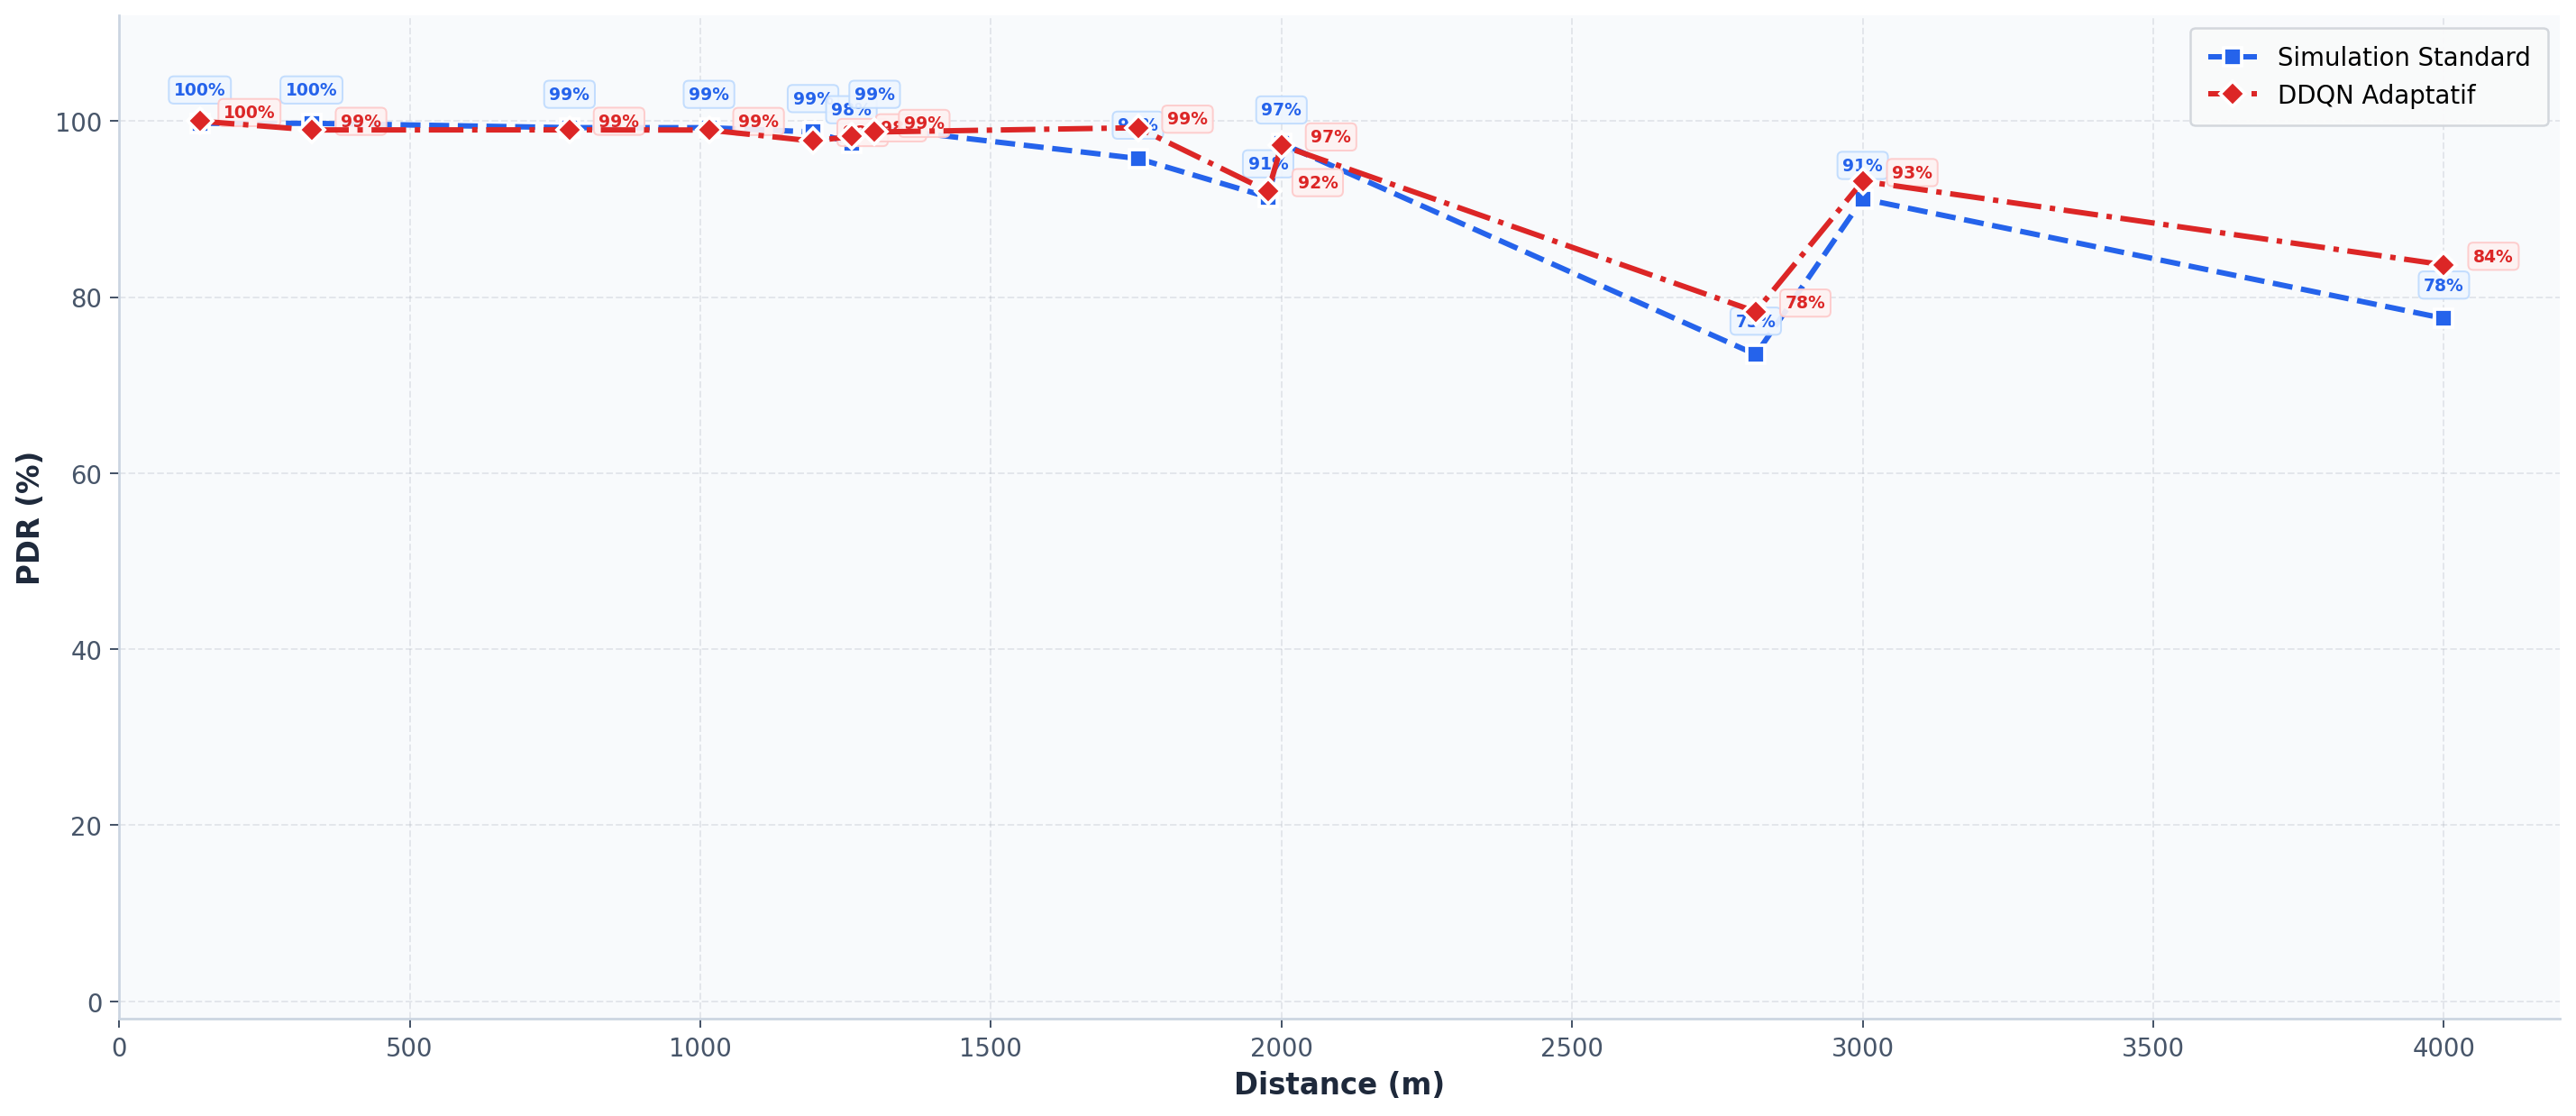
\includegraphics[width=1\textwidth]{images/validation/ddqn/dr/dr10_pdr_courbes.png}
		\caption{Comparaison PDR pour DR10 : Standard vs DDQN}
		\label{fig:dr10-pdr}
	\end{figure}
	
	\begin{figure}[H]
		\centering
		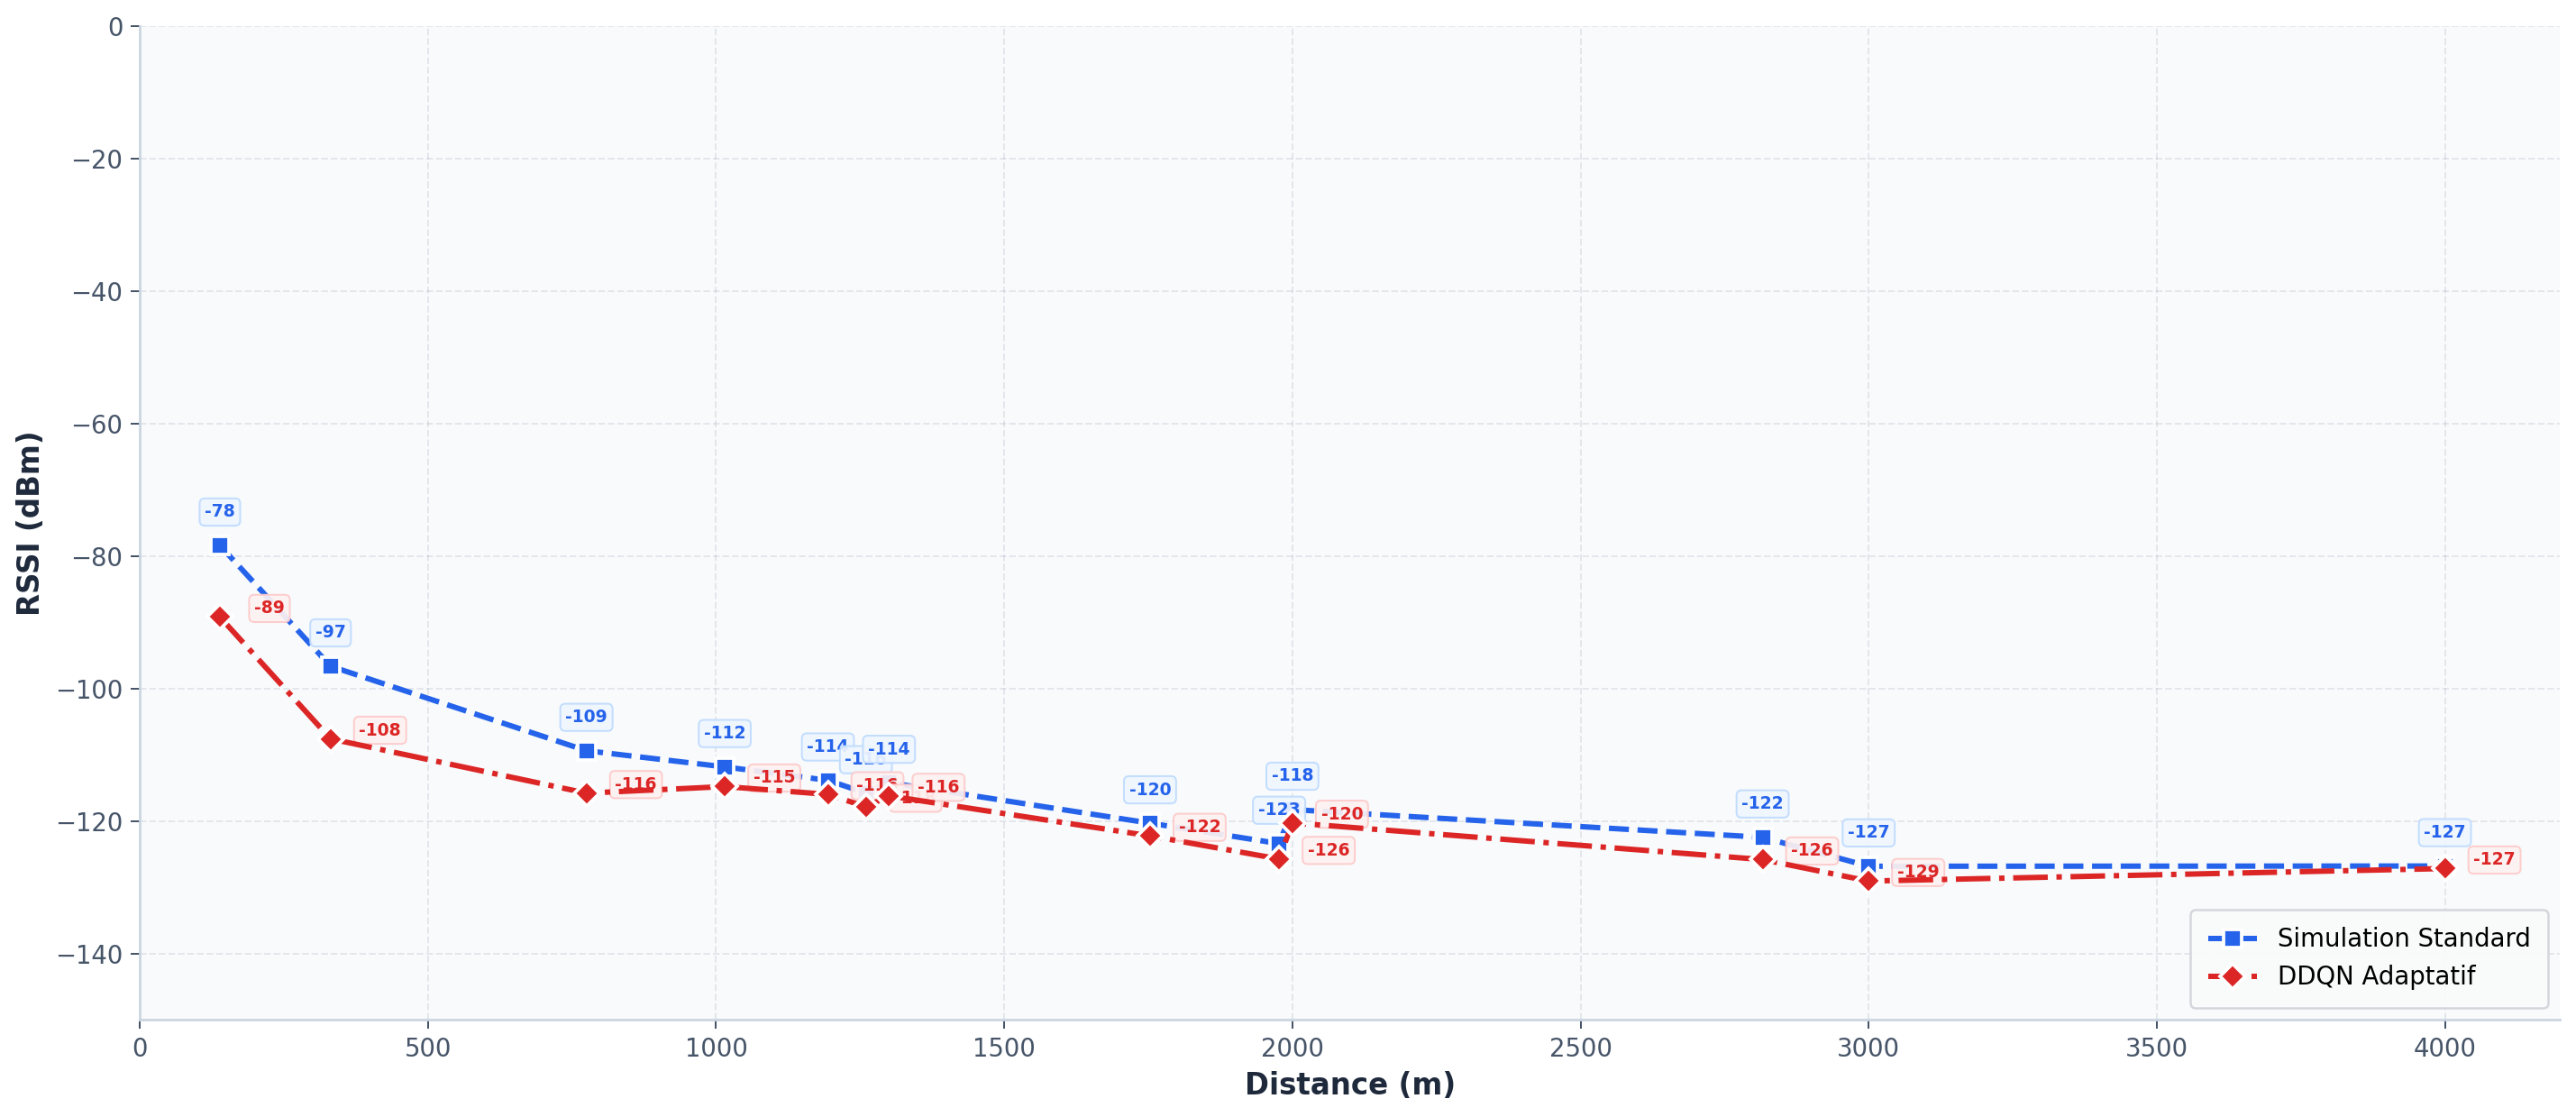
\includegraphics[width=1\textwidth]{images/validation/ddqn/dr/dr10_rssi_courbes.png}
		\caption{Comparaison RSSI pour DR10 : Standard vs DDQN}
		\label{fig:dr10-rssi}
	\end{figure}
	
	Le DDQN se montre également performant pour le DR10, avec un écart plus marqué que celui observé pour le DR8 (\ref{fig:dr8-pdr}). À 4000 m, le PDR atteint 84\% avec le DDQN, contre 78\% pour la simulation standard, soit un gain absolu de 6 points et une amélioration relative d'environ 7,6\%.
	
	\newpage
	\item \textbf{Analyse pour DR11 (CR 2/3, BW 336 kHz)}
	
	\begin{figure}[H]
		\centering
		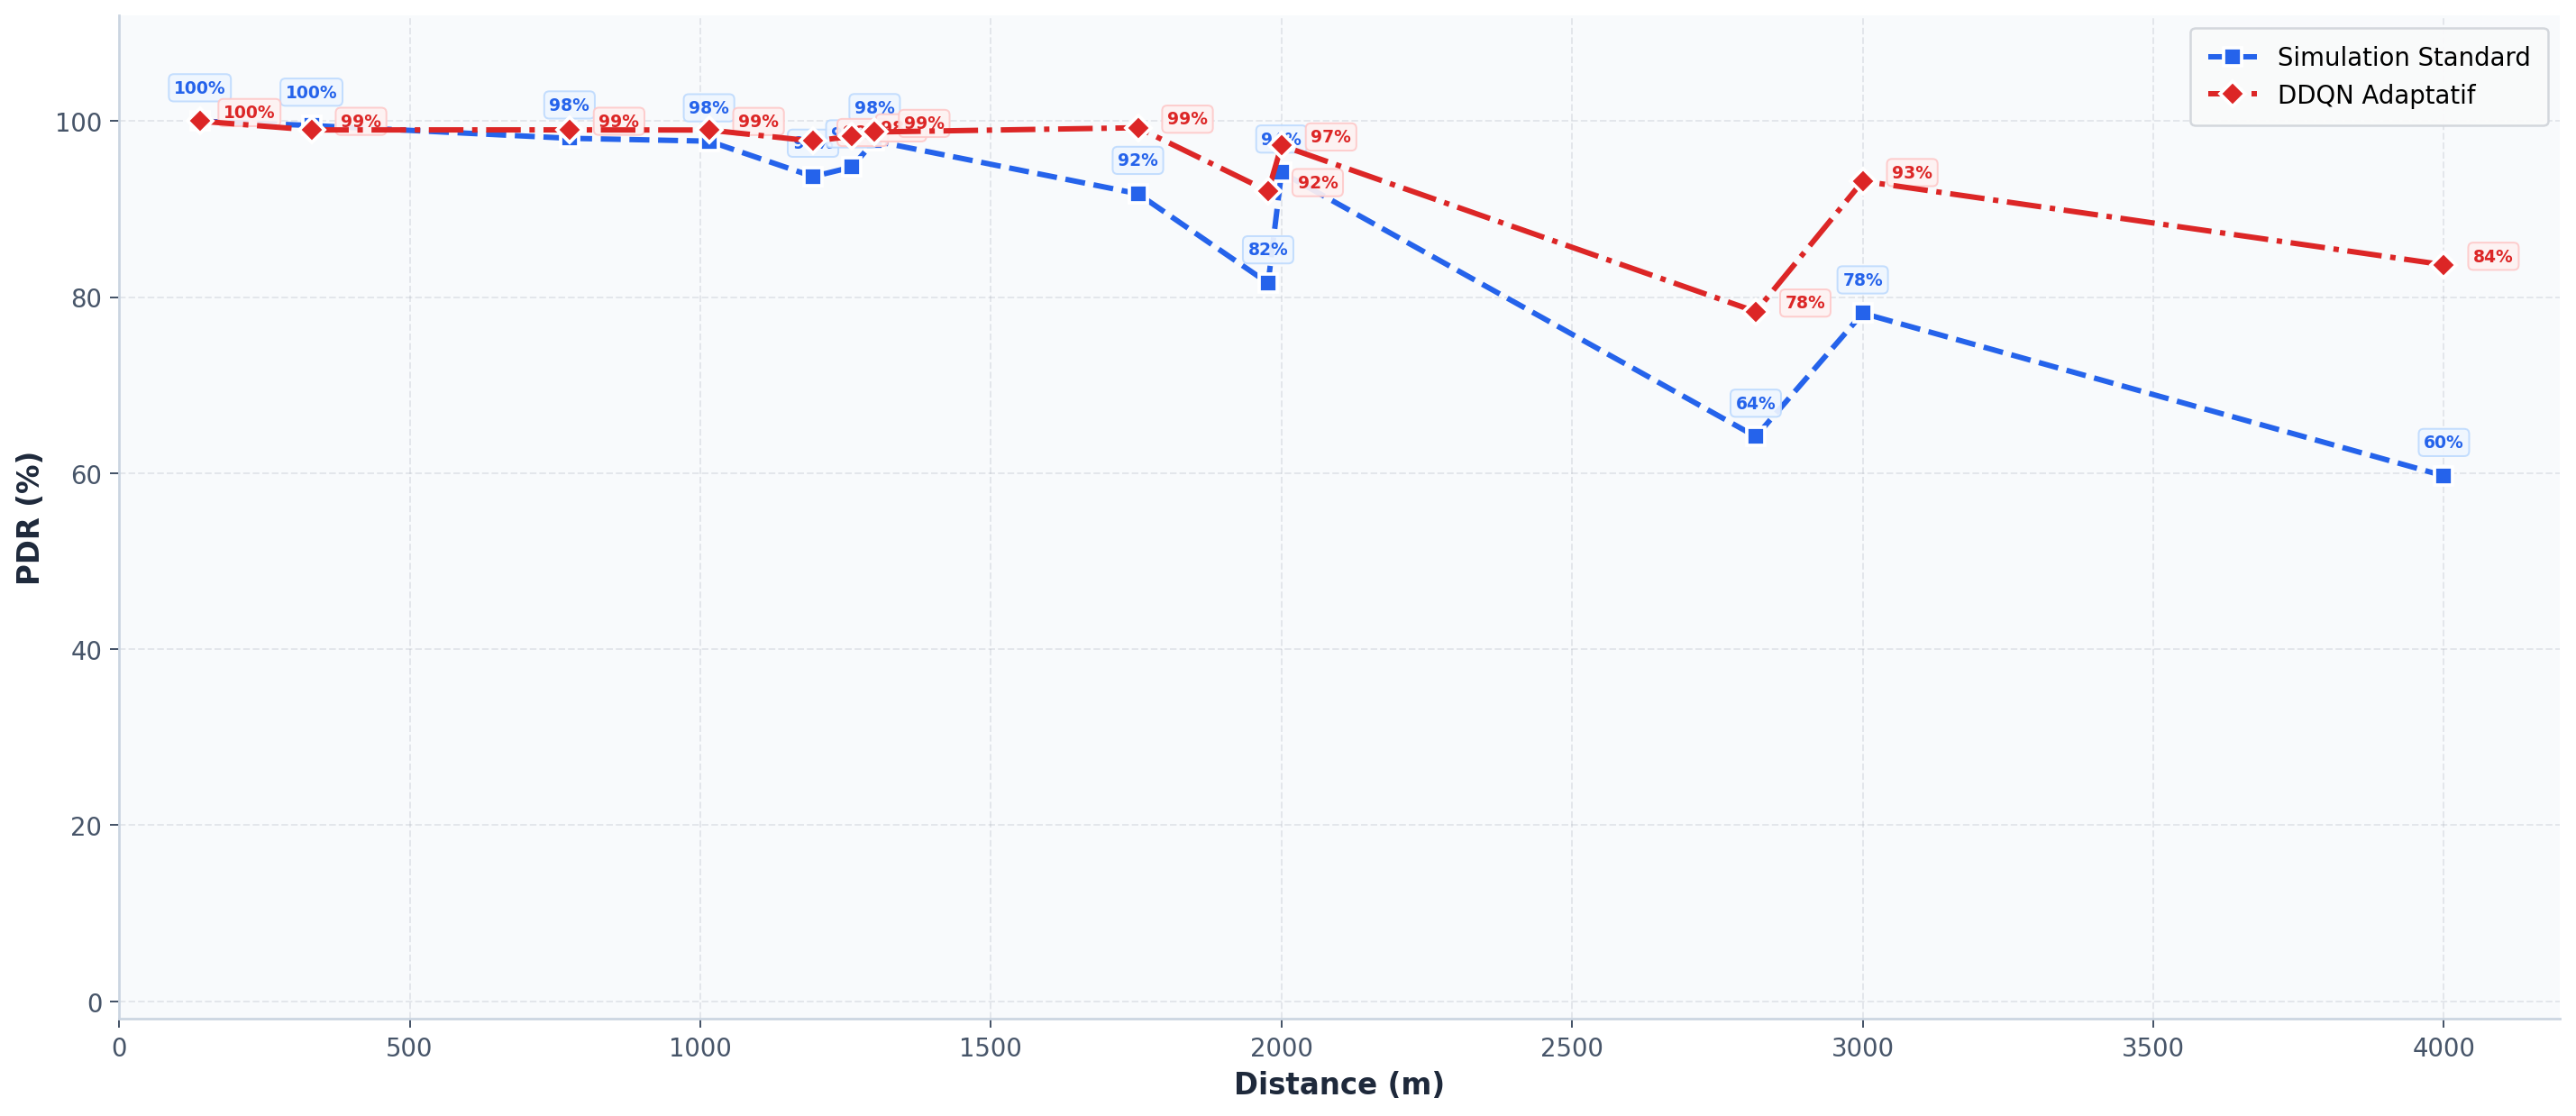
\includegraphics[width=1\textwidth]{images/validation/ddqn/dr/dr11_pdr_courbes.png}
		\caption{Comparaison PDR pour DR11 : Standard vs DDQN}
		\label{fig:dr11-pdr}
	\end{figure}
	
	\begin{figure}[H]
		\centering
		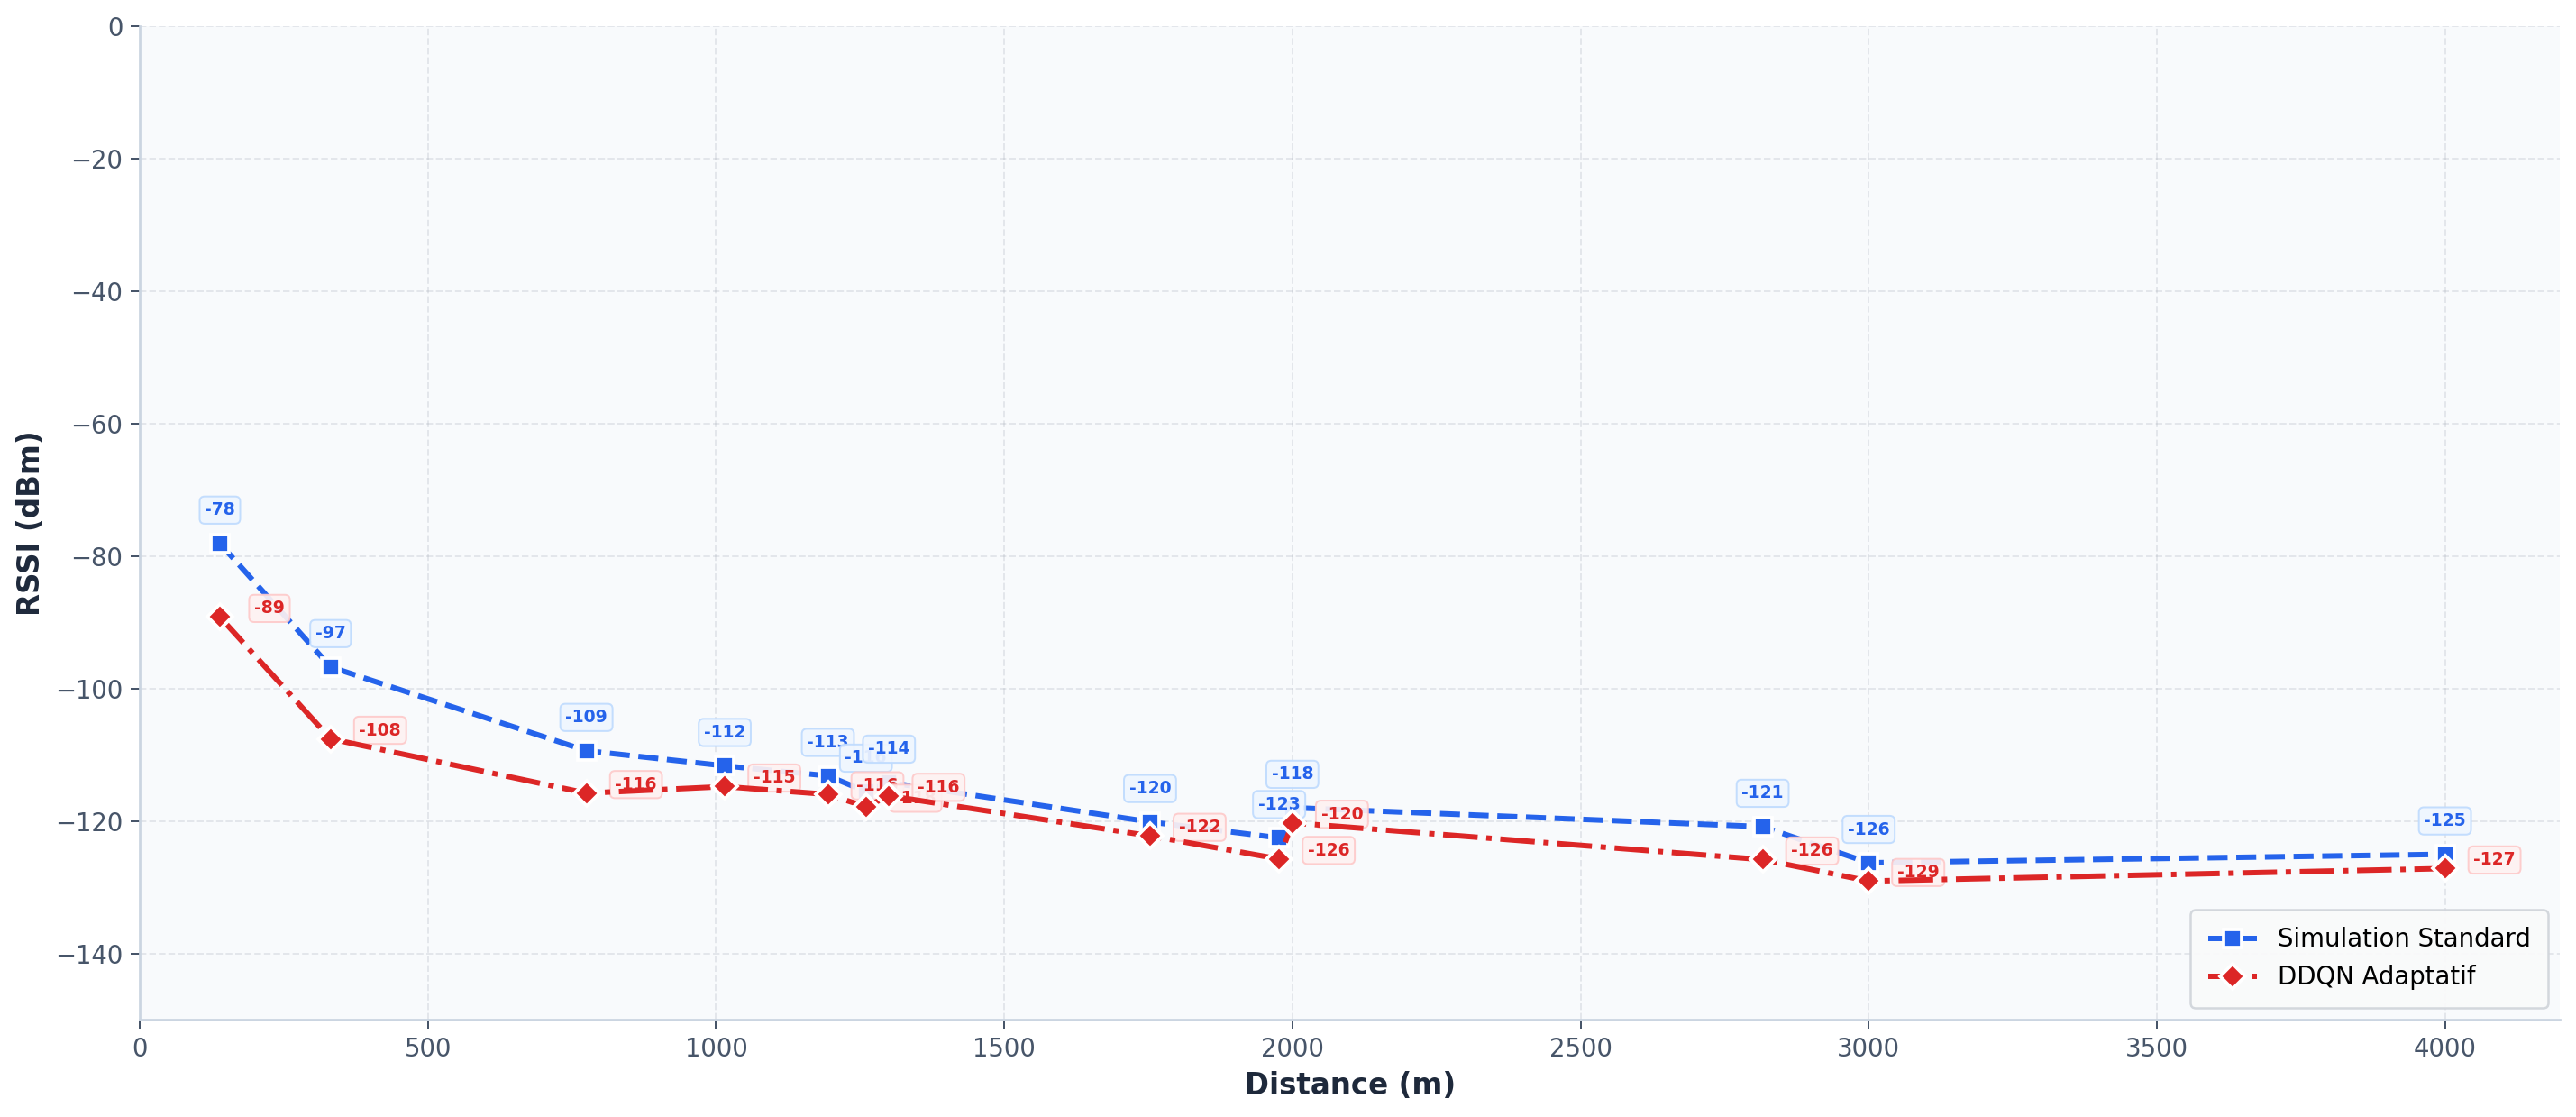
\includegraphics[width=1\textwidth]{images/validation/ddqn/dr/dr11_rssi_courbes.png}
		\caption{Comparaison RSSI pour DR11 : Standard vs DDQN}
		\label{fig:dr11-rssi}
	\end{figure}
	
	Pour le DR11, l'agent DDQN s'impose largement. Au-delà de 1000 m, il présente un taux de succès supérieur à celui du DR11 seul. À 4000 m, le PDR atteint 84\% avec le DDQN, contre 60\% pour le DR11, soit un gain absolu de 24 points et une amélioration relative d'environ 40\%.\\
	\\
	Un comportement similaire est observé concernant l'évolution du RSSI, quel que soit le DR. L'agent DDQN présente un RSSI plus faible sur l'ensemble des distances, avec un effet encore plus marqué sur les courtes distances. Cela illustre sa capacité à adapter dynamiquement la puissance d'émission.
\end{itemize}

\subsection{Analyse des performances par distance}

\begin{itemize}
	\item \textbf{Analyse du PDR}
	
	Le tableau \ref{tab:comparaison-pdr} présente la comparaison détaillée du taux de livraison (PDR) entre la simulation standard et l'agent DDQN pour les 13 distances évaluées. La colonne Standard représente la moyenne des 4 DR statiques.
	
	\begin{table}[H]
		\centering
		\caption{Comparaison du PDR : simulation standard vs agent DDQN}
		\label{tab:comparaison-pdr}
		\begin{tabular}{|c|c|c|c|c|}
			\hline
			\textbf{Distance (m)} & \textbf{Standard (\%)} & \textbf{DDQN (\%)} & \textbf{Variation (pts)} & \textbf{Taux (\%)}\\
			\hline
			\hline
			139  & 99,9 & 100,0 & +0,1 &\cellcolor{green!30} +0,1\\
			\hline
			331  & 99,7 & 99,0  & -0,7 & \cellcolor{red!30} -0,7 \\
			\hline
			775  & 99,2 & 99,0  & -0,2 & \cellcolor{red!30} -0,2\\
			\hline
			1015 & 98,7 & 99,0  & +0,3 &\cellcolor{green!30} +0,3\\
			\hline
			1194 & 97,1 & 97,7  & +0,6 &\cellcolor{green!30} +0,7\\
			\hline
			1260 & 97,5 & 98,3  & +0,8 &\cellcolor{green!30} +0,8\\
			\hline
			1300 & 98,6 & 98,8  & +0,2 & \cellcolor{green!30}+0,2\\
			\hline
			1753 & 95,7 & 99,2  & +3,5 & \cellcolor{green!30}+3,66\\
			\hline
			1977 & 89,1 & 92,0  & +2,9 &\cellcolor{green!30} +3,25\\
			\hline
			2000 & 97,1 & 97,2  & +0,1 &\cellcolor{green!30} +0,1\\
			\hline
			2816 & 72,6 & 78,4  & +5,8 &\cellcolor{green!30} +7,99 \\
			\hline
			3000 & 87,7 & 93,2  & +5,5 &\cellcolor{green!30}+6,27\\
			\hline
			4000 & 72,4 & 83,7  & +11,3 &\cellcolor{green!30} +15,6 \\
			\hline
			\hline
			\textbf{Moyenne} & \textbf{92,7} & \textbf{95,0} & \textbf{+2,3} & \cellcolor{green!30} \textbf{+2,48} \\
			\hline
		\end{tabular}
	\end{table}
	
	L'agent DDQN améliore le PDR dans 11 cas sur 13 (85\% des distances), avec une amélioration moyenne de 2,3 points. Les gains les plus significatifs sont observés aux longues distances : +11,3 points à 4000 m, +5,8 points à 2816 m et +5,5 points à 3000 m.
	
	\item \textbf{Analyse du débit}
	
	Le tableau suivant présente l'évolution du débit moyen de l'agent DDQN comparé au débit moyen bas (DR8/DR10) et haut (DR9/DR11) dans les mêmes conditions.
	
	\begin{table}[H]
		\centering
		\caption{Évolution du débit en fonction de la distance}
		\label{tab:debit_distance}
		\begin{tabular}{|c|c|c|c|c|}
			\hline
			\textbf{Distance (m)} &  \textbf{DR8/10 (bps)} & \textbf{DR9/11 (bps)} &   \textbf{Moyenne (bps)} & \textbf{DDQN (bps)} \\
			\hline
			139    & 89,59  & 142,05 & 115,82 & 142,05 \\
			\hline
			331    & 89,59  & 142,05 & 115,82 & 140,73 \\
			\hline
			775    & 89,59  & 142,05 & 115,82 & 90,11 \\
			\hline
			1015-4000 & 89,59  & 142,05 & 115,82  & 89,59 \\
			\hline
		\end{tabular}
	\end{table}
	Pour maximiser la fiabilité à longue distance, l'agent DDQN sacrifie le débit de manière délibérée, en privilégiant systématiquement les configurations les plus robustes (DR8/10).
		
	\item \textbf{Analyse de la puissance d'émission}
	
	Le tableau suivant présente l'évolution de la puissance de transmission utilisée par l'agent DDQN en fonction de la distance, comparativement à la puissance fixe de l'approche standard.
	
	\begin{table}[H]
		\centering
		\caption{Comparaison de la puissance d'émission}
		\label{tab:comparaison-puissance}
		\begin{tabular}{|c|c|c|c|}
			\hline
			\textbf{Distance (m)} & \textbf{Puiss. Standard (dBm)} & \textbf{Puiss. DDQN (dBm)} & \textbf{Réduction (\%)} \\
			\hline
			\hline
			139  & 14,0 & 3,0  & 78,6 \% \\
			\hline
			331  & 14,0 & 3,1  & 77,9 \% \\
			\hline
			775  & 14,0 & 7,6  & 45,7 \% \\
			\hline
			1015 & 14,0 & 11,1 & 20,7 \% \\
			\hline
			1194 & 14,0 & 11,9 & 15,0 \% \\
			\hline
			1260 & 14,0 & 12,0 & 14,3 \% \\
			\hline
			1300 & 14,0 & 12,0 & 14,3 \% \\
			\hline
			1753 & 14,0 & 12,0 & 14,3 \% \\
			\hline
			1977 & 14,0 & 12,0 & 14,3 \% \\
			\hline
			2000 & 14,0 & 12,0 & 14,3 \% \\
			\hline
			2816 & 14,0 & 12,0 & 14,3 \% \\
			\hline
			3000 & 14,0 & 12,0 & 14,3 \% \\
			\hline
			4000 & 14,0 & 14,0 & 0,0 \% \\
			\hline
			\hline
			\textbf{Moyenne} & \textbf{14,0} & \textbf{9,5} & \textbf{32,0 \%} \\
			\hline
		\end{tabular}
	\end{table}
	
	L'analyse de la puissance d'émission révèle une réduction moyenne de 32\%, avec des économies importantes aux courtes distances (jusqu'à 78,6\% à 139 m). Cette réduction de puissance contribue directement à l'efficacité énergétique globale du système.
	
	\newpage
	\item \textbf{Comparaison énergétique}
	
	Le tableau suivant présente la consommation énergétique de l'approche standard et de l'agent DDQN.
	
	\begin{table}[H]
		\centering
		\caption{Comparaison de l'énergie consommée par paquet}
		\label{tab:comparaison-energie}
		\begin{tabular}{|c|c|c|c|}
			\hline
			\textbf{Distance (m)} & \textbf{Énergie Std (mJ)} & \textbf{Énergie DDQN (mJ)} & \textbf{Variation (\%)} \\
			\hline
			\hline
			139  & 76,88 & 28,81  & \cellcolor{green!30} -62,5 \% \\
			\hline
			331  & 76,92 & 29,62  & \cellcolor{green!30} -61,5 \% \\
			\hline
			775  & 76,95 & 61,65  & \cellcolor{green!30} -19,9 \% \\
			\hline
			1015 & 76,91 & 77,14  & \cellcolor{red!30} +0,3 \% \\
			\hline
			1194 & 76,95 & 81,73  &\cellcolor{red!30} +6,2 \% \\
			\hline
			1260 & 76,98 & 82,51  &\cellcolor{red!30} +7,2 \% \\
			\hline
			1300 & 76,93 & 82,51  &\cellcolor{red!30} +7,3 \% \\
			\hline
			1753 & 76,86 & 82,51  &\cellcolor{red!30} +7,3 \% \\
			\hline
			1977 & 76,86 & 82,51  & \cellcolor{red!30}+7,3 \% \\
			\hline
			2000 & 76,88 & 82,51  & \cellcolor{red!30}+7,3 \% \\
			\hline
			2816 & 76,85 & 82,51  &\cellcolor{red!30} +7,4 \% \\
			\hline
			3000 & 77,00 & 82,54  & \cellcolor{red!30}+7,2 \% \\
			\hline
			4000 & 77,05 & 94,29  &\cellcolor{red!30} +22,4 \% \\
			\hline
			\hline
			\textbf{Moyenne} & \textbf{76,93} & \textbf{73,14} & \cellcolor{green!30} \textbf{-4,9 \%} \\
			\hline
		\end{tabular}
	\end{table}
	
	La consommation énergétique par paquet est réduite de 4,9\% en moyenne, avec des économies substantielles aux courtes distances, atteignant 62,5\% à 139 m. Aux distances intermédiaires, un léger surcoût de l'ordre de 6 à 7\% est observé, mais celui-ci est largement compensé par les gains de fiabilité obtenus sur le PDR.
	À 4000 m, le surcoût de 22,4\% s'explique par la nature même de la référence de comparaison. En effet, la simulation standard représente la moyenne des quatre DR statiques (DR8, DR9, DR10, DR11), tous émis à la puissance maximale de 14 dBm. Or, les configurations DR9 et DR11 (CR = 2/3) génèrent un temps d'antenne structurellement plus court que DR8 et DR10 (CR = 1/3), ce qui abaisse considérablement la consommation énergétique moyenne de référence. À l'inverse, l'agent DDQN, face à la dégradation du canal à longue distance, bascule délibérément vers les configurations les plus robustes (DR8/DR10, CR = 1/3), dont le temps d'antenne plus long entraîne une consommation par paquet plus élevée. Ce surcoût énergétique constitue donc un arbitrage intentionnel : il permet un gain de PDR de 11,3 points à 4000 m, soit une amélioration relative de 15,6\%, ce qui confirme la pertinence de la stratégie adoptée par l'agent dans les conditions de canal les plus défavorables.
	
\end{itemize}

\newpage
\subsection{Synthèse des gains apportés par le DDQN}

Ce tableau présente les apports de l'agent DDQN sur les plages de distance.

\begin{table}[H]
	\centering
	\caption{Synthèse des performances par plage de distance}
	\label{tab:synthese-plages}
	\begin{tabular}{|l|c|c|c|c|}
		\hline
		\textbf{Plage de distance} & \textbf{Cas} & \textbf{PDR (pts)} & \textbf{Puissance (dBm)} & \textbf{Énergie (\%)} \\
		\hline
		\hline
		Courte (< 1000 m)      & 3  & \cellcolor{red!30}-0,3 & \cellcolor{green!30}-9,4 & \cellcolor{green!30} -47,9 \% \\
		\hline
		Moyenne (1000-2000 m)  & 7  & \cellcolor{green!30} +1,1 & \cellcolor{green!30}-2,1 &\cellcolor{red!30} +6,1 \% \\
		\hline
		Longue (> 2000 m)      & 3  & \cellcolor{green!30}+7,5 & \cellcolor{green!30}-1,5 & \cellcolor{red!30}+12,3 \% \\
		\hline
	\end{tabular}
\end{table}

Cette analyse par plage de distance révèle la stratégie adaptative optimale de l'agent DDQN :
\begin{itemize}
	\item \textbf{Courtes distances} : Économies d'énergie massives sans compromis sur la fiabilité
	\item \textbf{Distances moyennes} : Investissement énergétique modéré pour un gain de PDR significatif
	\item \textbf{Longues distances} : Forte amélioration de la fiabilité pour un surcoût énergétique acceptable
\end{itemize}

Le tableau \ref{tab:synthese-gains} synthétise les gains quantitatifs apportés par notre solution, avec une moyenne globale sur toutes les distances.

\begin{table}[H]
	\centering
	\caption{Synthèse globale des gains apportés par l'agent DDQN}
	\label{tab:synthese-gains}
	\begin{tabular}{|l|c|c|c|}
		\hline
		\textbf{Métrique} & \textbf{Standard} & \textbf{DDQN} & \textbf{Gain} \\
		\hline
		\hline
		PDR moyen (\%) & 92,7 & 95,0 & \textbf{+2,48\%} \\
		\hline
		Puissance moyenne (dBm) & 14,0 & 9,5 & \textbf{-32,14 \%} \\
		\hline
		Énergie moyenne par paquet (mJ) & 76,93 & 73,14 & \textbf{-4,9 \%} \\
		\hline
		Énergie minimale (mJ) & 76,88 & 28,81 & \textbf{-62,5 \%} \\
		\hline
		PDR à 4000 m (\%) & 72,4 & 83,7 & \textbf{+15,6\%} \\
		\hline
		Cas favorables (PDR) & 2/13 & 11/13 & \textbf{84,61 \%} \\
		\hline
	\end{tabular}
\end{table}

Ces gains s'expliquent par ces mécanismes clés :
\begin{enumerate}
	\item \textbf{Évitement du surdimensionnement} : Ajustement fin de la puissance avec des réductions jusqu'à 78,6\%
	\item \textbf{Sélection adaptative du DR} : Basculement progressif des DR à haut débit vers les DR robustes
\end{enumerate}

\section{Limites et perspectives}

\subsection{Limites de notre solution}

Bien que notre approche ait démontré son efficacité en termes de fiabilité, d'adaptativité et d'économies d'énergie, plusieurs limites doivent être soulignées :

\begin{itemize}
	\item \textbf{Modèle de canal simplifié.} Le modèle de propagation utilisé repose sur une approche \textit{log-distance} avec un ombrage (\textit{shadowing}). Bien que validé par des données terrain récentes \cite{lrfhss_comparaison}, ce modèle ne capture pas les variations temporelles rapides du canal (évanouissements multi-trajets, interférences dynamiques) ni les conditions environnementales changeantes (météo, obstacles mobiles). En conséquence, la fidélité du simulateur pourrait être réduite dans des scénarios plus complexes.
	
	\item \textbf{Agent DDQN entraîné hors ligne.} L’agent a été entraîné dans un environnement à très faible densité, puis ses poids ont été sauvegardés pour la phase d'évaluation. Par conséquent, son comportement face à un trafic réseau plus dense reste à déterminer. De plus, l'apprentissage hors ligne ne permet pas à l'agent de s'adapter en temps réel à des changements imprévus de l'environnement.
	
	\item \textbf{Modèle énergétique partiel.} Notre estimation de la consommation énergétique se limite à l'énergie d'émission, calculée à partir de la puissance de transmission et du temps d'antenne. Elle n'inclut pas la consommation liée à la réception, ni aux échanges protocolaires. L'énergie réelle par paquet utile est donc sous-estimée. De plus, notre évaluation ne mesure pas l'impact énergétique des échecs de transmission (et des retransmissions associées) sur le budget global du nœud.
	
	\item \textbf{Généralisation limitée.} Notre étude s'est concentrée sur un environnement unique (d'après les données de validation), une taille de la charge utile fixe de 1 octet et des nœuds statiques. La validité de nos conclusions dans d'autres contextes (charge utiles longues, mobilité) reste à démontrer.
\end{itemize}



\subsection{Perspectives}

Les limites identifiées précédemment ouvrent naturellement plusieurs axes d'amélioration et extensions pour des travaux futurs :

\begin{itemize}
	\item \textbf{Modélisation plus fine du canal.} Une première perspective consisterait à enrichir le modèle de propagation en intégrant des variations temporelles de l'évanouissement lent (\textit{shadowing}) ou des modèles d'évanouissement plus réalistes (Rice, Nakagami). L'ajout d'un modèle d'interférences permettrait également de simuler des environnements avec plus de réalisme.
	
	\item \textbf{Agent adaptatif et apprentissage en ligne.} L'agent DDQN gagnerait à être évalué dans des conditions plus variées : topologies aléatoires multiples, trafic variable, présence d'autres technologies (LoRa classique). Une évolution majeure serait le passage à un apprentissage en ligne (\textit{online learning}) permettant à l'agent d'ajuster sa politique en temps réel face à des changements environnementaux. L'exploration d'autres architectures d'apprentissage pourrait également être envisagée.
	
	\item \textbf{Modèle énergétique complet :} Une amélioration significative consisterait à développer un modèle énergétique plus exhaustif, conforme à la spécification LoRaWAN classe A. Celui-ci intégrerait la consommation en mode réception (écoute du canal), les échanges d'acquittements, l'énergie de réveil et d'échange protocolaire. Cette extension permettrait d'estimer plus précisément la durée de vie des nœuds et de valider les gains énergétiques annoncés.
	
	\item \textbf{Validation multi-environnements.} Une perspective importante serait de valider notre approche sur plusieurs jeux de données correspondant à des environnements variés (urbain, rural, industriel, intérieur) et des conditions météorologiques différentes. Des campagnes de mesures dédiées, avec des charges utiles réalistes (10 à 50 octets) et des scénarios de mobilité, constitueraient une validation terrain plus impactante.
	
	\item \textbf{Passage à l'échelle et déploiement réel.} Enfin, le comportement de l'agent dans des réseaux de grande taille (plusieurs centaines de nœuds) reste à étudier, notamment en termes de complexité computationnelle et d'adaptation aux interférences. À plus long terme, une implémentation sur plateforme réelle (carte LoRaWAN, gateway) permettrait de valider expérimentalement les gains observés en simulation et d'étudier les défis pratiques liés au déploiement de l'algorithme d'apprentissage.
	
\end{itemize}



\section{Conclusion}

Ce chapitre a présenté une évaluation approfondie de l'agent DDQN pour l'optimisation des transmissions LR-FHSS. En confrontant ses performances à celles de la simulation standard sans DDQN sur un ensemble de distances, nous avons démontré des gains significatifs sur tous les axes de performance, à savoir la fiabilité, l'efficacité énergétique et l'adaptabilité. Nous avons également exposé les limites de notre approche et donné les futures directions d'amélioration.
	\newpage
\chapter*{CONCLUSION GÉNÉRALE}
\addcontentsline{toc}{chapter}{CONCLUSION GÉNÉRALE}

Ce travail de recherche a été consacré à l'optimisation des transmissions \textbf{LR-FHSS} à l'aide de l'apprentissage par renforcement profond (\textit{Deep Reinforcement Learning}). Face aux défis croissants de passage à l'échelle et d'efficacité énergétique des réseaux IoT, nous avons proposé une approche dynamique capable d'adapter intelligemment les paramètres de transmission aux conditions changeantes du canal radio.

La première phase de notre étude a permis la conception et la validation d'un simulateur événementiel développé en Python. En respectant rigoureusement les spécifications techniques de la norme LR-FHSS et en confrontant nos résultats à des données réelles, nous avons obtenu une erreur quadratique moyenne (RMSE) de \textbf{12,14 \%}, garantissant ainsi la fiabilité des évaluations de performances menées par la suite.

L'implémentation d'un agent fondé sur l'algorithme \textbf{Double Deep Q-Network (DDQN)} a ensuite démontré la pertinence de l'intelligence artificielle face aux méthodes d'allocation statiques. Nos résultats mettent en évidence une amélioration du taux de livraison des paquets (PDR) de \textbf{2,48\%} en moyenne, tout en réalisant une réduction significative de la puissance d'émission de \textbf{32 \%}. Cette optimisation se traduit par une diminution de la consommation énergétique globale de \textbf{4,9 \%}, confirmant la viabilité de cette approche pour prolonger l'autonomie des nœuds capteurs dans des environnements contraints.

Malgré ces avancées significatives, ce travail ouvre la voie à plusieurs perspectives de recherche. Une modélisation encore plus fine du canal radio pourrait être envisagée en intégrant des modèles d'évanouissement (\textit{fading}) complexes, ainsi qu'une gestion plus précise des variations temporelles de l'ombrage (\textit{shadowing}). Par ailleurs, l'inclusion du surcoût protocolaire réel et des mécanismes de retransmission permettrait d'affiner le bilan énergétique global du système.

En somme, cette étude démontre que l'apprentissage par renforcement constitue un levier technologique indispensable pour l'évolution des réseaux LPWAN vers plus d'autonomie et d'efficacité spectrale. À terme, le passage de la simulation au déploiement sur des passerelles de production représentera une étape décisive pour soutenir la croissance de l'Internet des Objets.
	
	% --------- BIBLIOGRAPHIE ---------
	\newpage
	
	
	\printbibliography
	
	\addcontentsline{toc}{chapter}{RÉFÉRENCES ET BIBLIOGRAPHIE}
	
	\newpage
	
	% --------- TABLE DES MATIÈRES ---------
	\cleardoublepage
	\renewcommand{\contentsname}{TABLE DES MATIÈRES} % Nouveau titre
	\etocsetnexttocdepth{3}                         % On affiche tout (jusqu'aux subsubsections)
	\tableofcontents
	\addcontentsline{toc}{chapter}{TABLE DES MATIÈRES}
	
	
\end{document}